\mode<article>{\usepackage{fullpage}}
%\mode<presentation>{\usetheme{CEA}}
\mode<presentation>{\usepackage{beamerthemeCeaList2012Red}}
% everyone:
\usepackage[english]{babel}
\usepackage{pgf}
\usepackage{graphicx}
\usepackage{pstricks}
\usepackage{pdfpages}
\usepackage{listings}
\usepackage{verbatim}
\usepackage{tikz}
\usetikzlibrary{arrows}

\mode<article> {
	\usepackage[center]{caption}
	\usepackage{hyperref}%                   % Utilisation de HyperTeX

	\hypersetup{
		pdfauthor   = {Gilles Mouchard, R\'eda Nouacer, Daniel Gracia P\'erez},%
		pdftitle    = {UNISIM Virtual Platforms Training},%
		pdfsubject  = {UNISIM-VP},%
		pdfkeywords = {simulation framework, architectural exploration, embedded system design, system verification},%
		pdfcreator  = {rubber},%
		pdfproducer = {rubber}
	}
}
%%\usepackage{xmpmulti}
%%\pgfdeclareimage[height=1cm]{myimage}{filename}

\mode<article> {
	\setjobnamebeamerversion{main.beamer}
}


\title{SystemC (VP3) \& SystemC TLM Tutorial (VP4)}
\author{Gilles Mouchard \\ R\'eda Nouacer \\ Daniel Gracia P\'erez}
\date{March 19, 2015}

%\usetheme{CEA}
\usepackage{beamerthemeCeaList2012Red}

\begin{document}
\mode<presentation>{
\lstset{% general command to set parameter(s)
language=c++,
basicstyle=\tiny, % print whole listing tiny
keywordstyle=\color{black}\bfseries, % bold black keywords
identifierstyle=, % nothing happens
commentstyle=\color{blue}, % white comments
stringstyle=\ttfamily, % typewriter type for strings
showstringspaces=false,
tabsize=4,
breaklines=true,
numbers=left,
framexleftmargin=7.5mm,
xleftmargin=0.13\textwidth,
xrightmargin=0.1\textwidth,
frame=tlbr}
}
\mode<article>{
\lstset{% general command to set parameter(s)
language=c++,
basicstyle=\footnotesize, % print whole listing small
keywordstyle=\color{black}\bfseries, % bold black keywords
identifierstyle=, % nothing happens
commentstyle=\color{blue}, % white comments
stringstyle=\ttfamily, % typewriter type for strings
showstringspaces=false,
tabsize=4,
breaklines=true,
numbers=left,
framexleftmargin=7.5mm,
xleftmargin=0.13\textwidth,
xrightmargin=0.1\textwidth,
frame=tlbr}
}
% \lstset{language=c++,basicstyle={\ttfamily\footnotesize},tabsize=4,breaklines=true,numbers=left,framexleftmargin=7.5mm,xleftmargin=0.13\textwidth,xrightmargin=0.1\textwidth,frame=tlbr}
\maketitle

\mode<article>{
\chapter*{Outline}
}

\mode<presentation>{
\part{Outline}
}

\mode<presentation>{
\begin{frame}
	\frametitle{Outline}
	\begin{itemize}
		\item Introduction (VP3)
		\item SystemC basics/CLM (VP3)
		\item SystemC TLM (VP4)\newline
		\item {\color{blue}\ldots and your questions}
	\end{itemize}
\end{frame}
}

\mode<article>{
Welcome to the SystemC tutorial.
We will introduce you to the exciting world of SystemC and the possibilities opened to you with SystemC Transaction Level Modelling (aka TLM).
We start with a presentation on what is SystemC and what you can use it for.
Then the basics of SystemC programming will be introduced, so you can start coding SystemC cycle level models.
The third part introduces SystemC TLM programming model, and more concretely TLM 2.0.

%Once the basics have been introduced, we will give an overview of the different existent frameworks that use SystemC.
%A special section will be reserved for the UNISIM simulation framework.
%More on them at the end of the tutorial.

% \begin{figure}[!h]
% 	\begin{center}
% 		\includegraphics[page=1,height=6cm]{main_beamer.pdf}
% 	\end{center}
% 	\caption{Outline slide.}
% 	\label{slide:outline}
% \end{figure}
}

\newpage

\mode<article>{
\tableofcontents
\listoffigures
\listoftables
}

\mode<article>{
\chapter{Introduction}
}

\mode<presentation>{
\part{Introduction}
}

\mode<presentation>{
\begin{frame}
	\frametitle{Introduction}
	\begin{block}{From the \emph{``SystemC 2.0 User's Guide''}:}
		\begin{center}
			``A C++ class library and methodology that you can use to effectively create a cycle-accurate model of software algorithms, hardware architecture, and interfaces of your SoC (System On a Chip) and system-level designs.''
		\end{center}
	\end{block}
	\begin{itemize}
		\item<2-> Really, what's SystemC?
		\begin{itemize}
			\item<2-> The different abstraction levels
		\end{itemize}
		\item<2-> Technically speaking
		\item<2->
		\item<2-> Conclusion
	\end{itemize}
\end{frame}
}

\mode<article>{
As stated in the \emph{``SystemC 2.0 User's Guide''} by the Accellera Consortium, we can define SystemC as:
\begin{quote}
	``A C++ class library and methodology that you can use to effectively create a cycle-accurate model of software algorithms, hardware architecture, and interfaces of your SoC (System On a Chip) and system-level designs.''
\end{quote}
Ok, this already says us what is the purpose of SystemC: create software models of SoCs and system-level designs. 
For that purpose SystemC provides a C++ class library and methodology\footnote{Yes, it provides a methodology, but it is focused at the component model. Actually, you will need to extend the SystemC methodology to define how the system components communicate.}.

The ``cycle-accurate'' part of the definition is a little bit outdated.
Currently, SystemC allows you not only to create cycle-accurate models, but for example purely functional models.
We will see in sligthly more detail which kind of models you can create with SystemC\footnote{Or at least the main ones. As we previously mentioned, SystemC is in constant evolution.}.

In the following sections we will try to define a little bit more in detail what is SystemC, and a rough view of the models you can create with it.
A more detailed description of those models  will be given in the following chapters.

% \begin{figure}[!h]
% 	\begin{center}
% 		\includegraphics[page=6,height=6cm]{main_beamer.pdf}
% 	\end{center}
% 	\caption{SystemC definition.}
% \end{figure}
}

\section{Really, what's SystemC?}
\mode<presentation>{
\begin{frame}
	\frametitle{Really, what's SystemC?}
	\begin{itemize}
		\item SystemC is proposed as a single ``\textbf{\textit{language}}'' to model your software/hardware platform at different layers of abstraction.
	\end{itemize}
	\begin{center}
		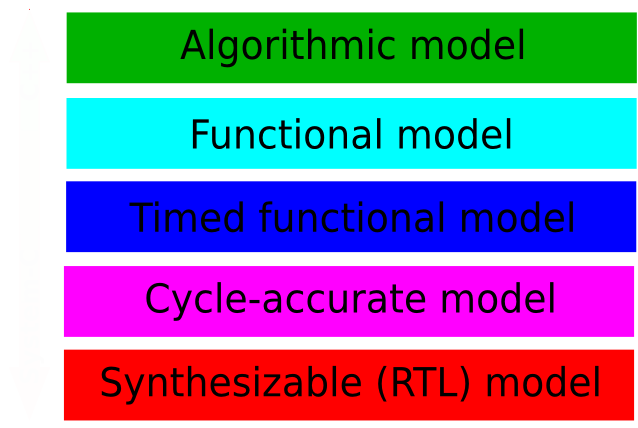
\includegraphics[width=0.8\textwidth]{introduction/figures/abstraction_layers-0.pdf}
	\end{center}
\end{frame}

\begin{frame}
\frametitle{Really, what's SystemC?}
	\begin{itemize}
		\item SystemC is proposed as a single ``\textbf{\textit{language}}'' to model your software/hardware platform at different layers of abstraction.
	\end{itemize}
	\begin{center}
		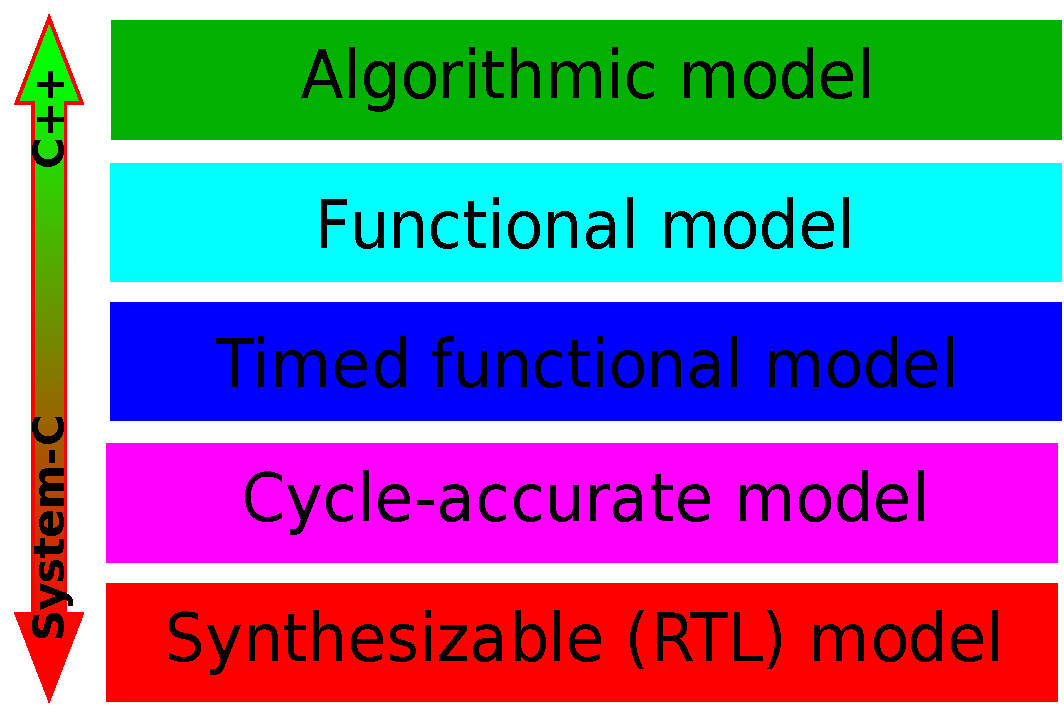
\includegraphics[width=0.8\textwidth]{introduction/figures/abstraction_layers-1.pdf}
	\end{center}
\end{frame}

\begin{frame}
	\frametitle{The abstraction levels: Algorithm}
	\begin{itemize}
		\item<1-> It defines what your system does.
		\item<1-> For example it can be described as a simple C++ program that computes Fibonacci.
	\end{itemize}
	\begin{figure}[h]
		\lstinputlisting{introduction/fibonacci.cc}
	\end{figure}
\end{frame}

\begin{frame}
	\frametitle{The abstraction levels: Functional}
	\begin{itemize}
		\item<1-> It defines how your system does what it is supposed to.
		\item<1-> The different system blocks appear at this stage.
		\item<1-> Continuing the Fibonacci example:
	\end{itemize}
	\begin{figure}[h]
		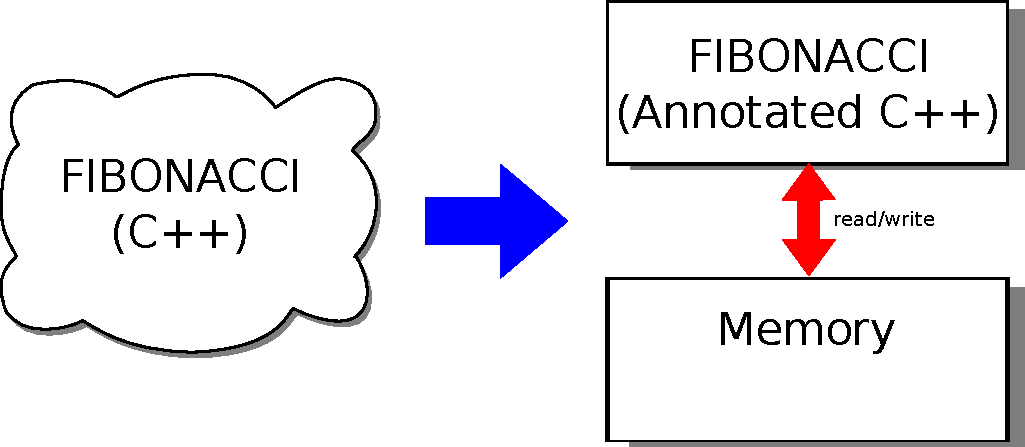
\includegraphics[width=0.8\textwidth]{introduction/figures/fibonacci_algo_to_functional_level.pdf}
	\end{figure}
\end{frame}

\begin{frame}
	\frametitle{The abstraction levels: Functional (II)}
	\begin{figure}[h]
		\lstinputlisting{introduction/fibonacci_annotated_presentation_1.cc}
	\end{figure}
\end{frame}

\begin{frame}
	\frametitle{The abstraction levels: Functional (II)}
	\begin{itemize}
		\item<1-> The {\color{red}read} and {\color{red}write} methods are responsible of sending messages using the SystemC primitives (which we will ignore for the moment).
	\end{itemize}
	\begin{figure}[h]
		\lstinputlisting{introduction/fibonacci_annotated_presentation_2.cc}
	\end{figure}
\end{frame}

\begin{frame}
	\frametitle{The abstraction levels: Timed functional}
	\begin{itemize}
		\item<1-> Adds time to the functional model, allowing you to model concurrency and resources constraints of your system. 
		\item<1-> The time description does not need to be precise,for example you can use average access times.
	\end{itemize}
	\begin{figure}[h]
		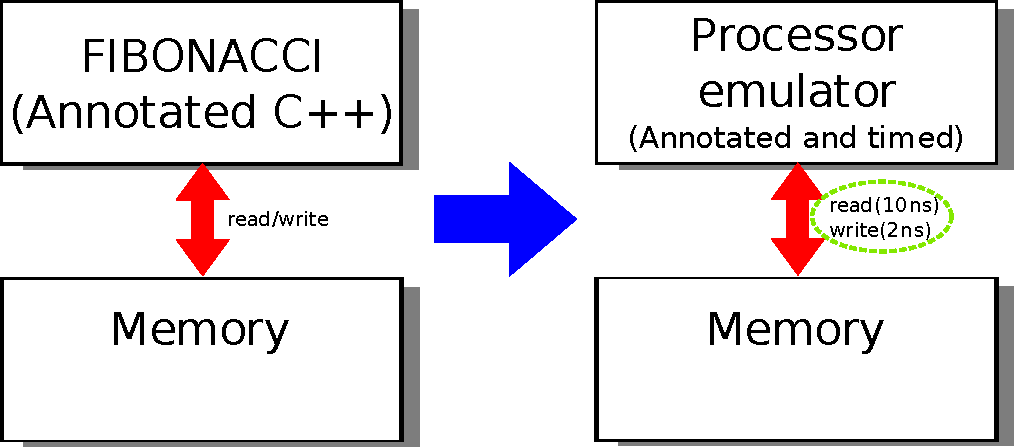
\includegraphics[width=0.8\textwidth]{introduction/figures/fibonacci_functional_to_timed_level.pdf}
	\end{figure}
\end{frame}

\begin{frame}
	\frametitle{The abstraction levels: Cycle-accurate}
	\begin{itemize}
		\item<1-> At this level time is very detailed, and matches closely that of the final system.
		\item<1-> Modeling at this level may require to write a new functional model.
	\end{itemize}
	\begin{figure}[h]
		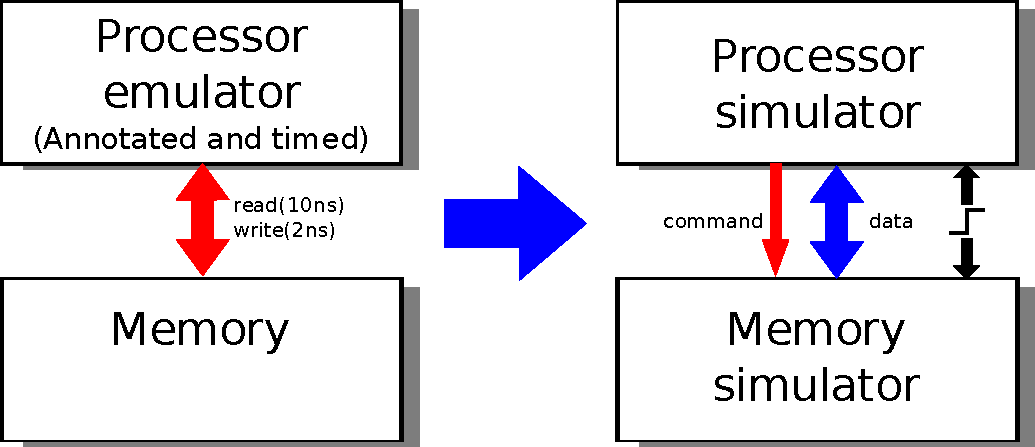
\includegraphics[width=0.8\textwidth]{introduction/figures/fibonacci_timed_to_cycle_level.pdf}
	\end{figure}
\end{frame}

\begin{frame}
	\frametitle{The abstraction levels: Synthesizable (RTL)}
	\begin{itemize}
		\item<1-> At this level the description is so detailed that the system can be synthetized.
	\end{itemize}
	\begin{figure}[h]
		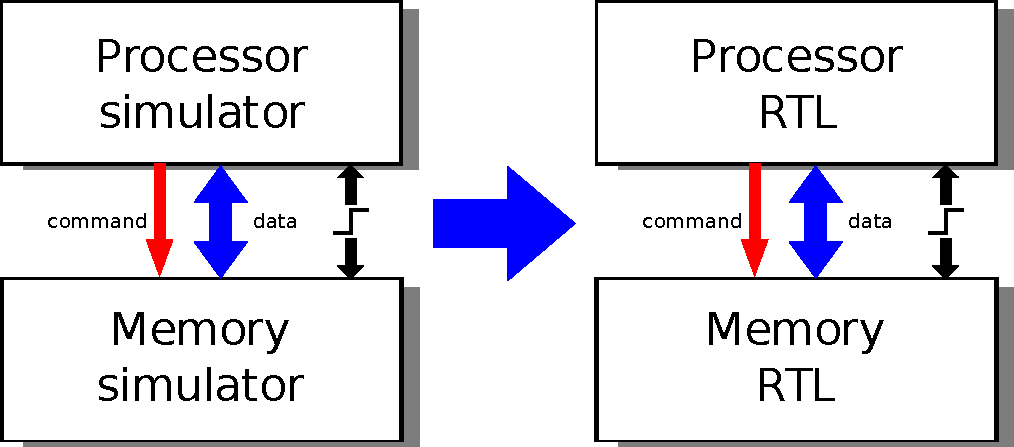
\includegraphics[width=0.8\textwidth]{introduction/figures/fibonacci_cycle_to_rtl_level.pdf}
	\end{figure}
\end{frame}
}

\mode<article>{
% \begin{figure}[!h]
% 	\begin{center}
% 		\includegraphics[page=6,height=6cm]{main_beamer.pdf}
% 	\end{center}
% 	\caption{Really, what's SystemC?}
% \end{figure}

\begin{figure}[!h]
	\begin{center}
		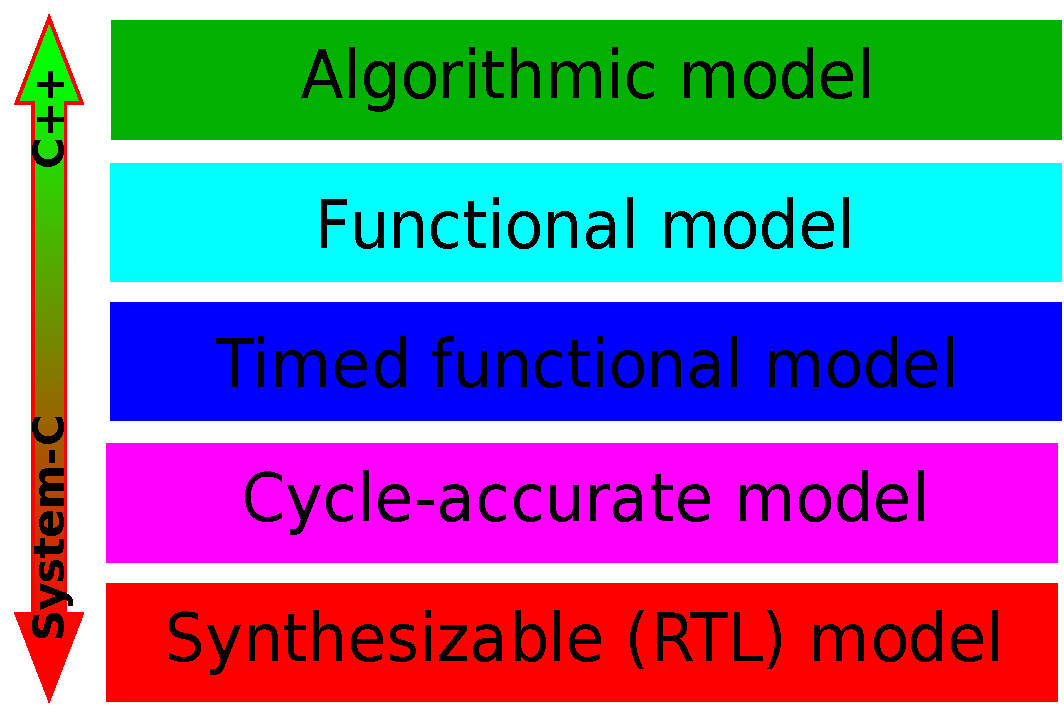
\includegraphics[width=0.8\textwidth]{introduction/figures/abstraction_layers-1.pdf}
	\end{center}
	\caption{Typical modeling levels of abstraction.}
	\label{fig:abstraction_layers}
\end{figure}

SystemC provides us with a single \emph{``language''} that allows us to model software/hardware platforms at different levels of abstraction.
Figure~\ref{fig:abstraction_layers} shows typical levels of abstraction when modeling software/hardware systems:
\begin{description}
	\item[Algorithm level:] it defines what your system does.
		For example, the algorithms implying the decoding of an MPEG4 flow into images.
	\item[Functional level:] it defines how your system does what it is supposed to do.
		Here you start to define the different blocks that compose your system: memories, processing elements, their connections, \ldots.
		Then you define how they communicate with each other, that is what is the communication sequence between your system components.
	\item[Timed functional level:] this model adds time to the functional model, allowing you to model concurrency and resources constraints of your system.
		The time description does not need to be precise, for example you can use average access times.
	\item[Cycle-accurate level:] this could be described as a very accurate timed functional model.
	\item[Synthetizable (RTL) level:] up to this level of abstraction, the description of components that composed the system did not need to be synthetizable.
		This level of abstraction provides a system that can be produced.
\end{description}

\begin{figure}[htb]
	\begin{center}
		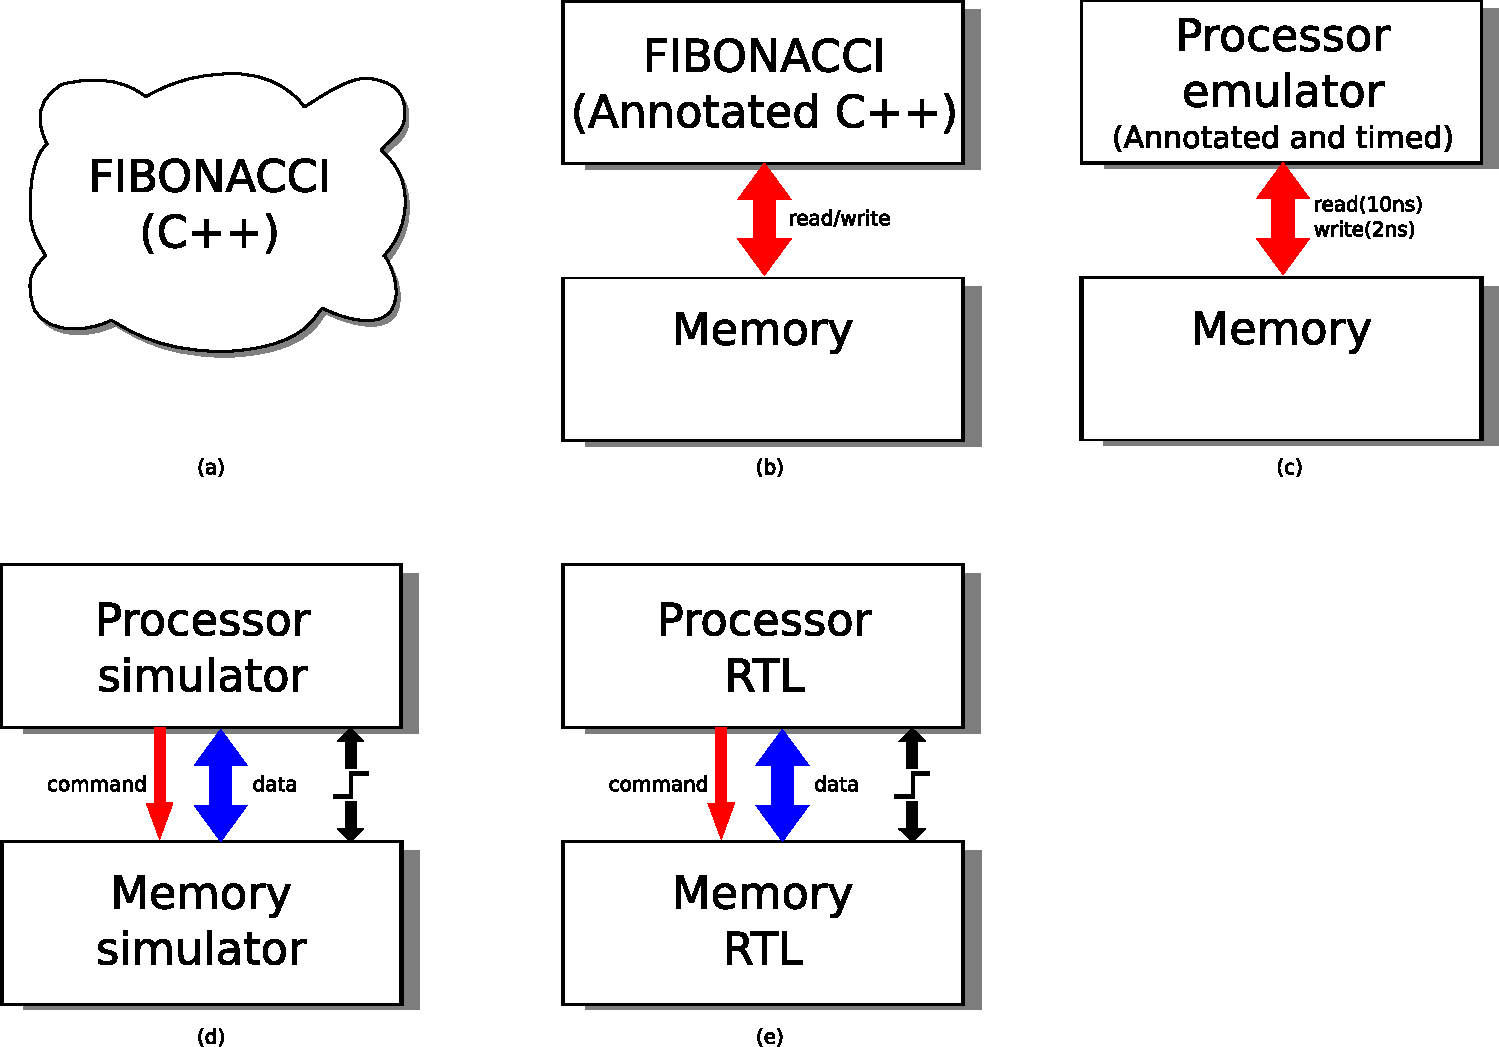
\includegraphics[width=0.8\textwidth]{introduction/figures/abstraction_level_example.pdf}
	\end{center}
	\caption{Example of a system represented at different levels of abstraction: (a) algorithm, (b) functional, (c) timed functional, (d) cycle-accurate, and (e) synthetizable levels.}
	\label{fig:abstraction_level_example}
\end{figure}

As SystemC is defined as an extension of the C++ programming language, the more abstract you are (the closer you are to the algorithm model) the less dependent you are in SystemC.
The more concrete your model is the more it will depend on SystemC. 
Actually, an algorithm model might be purely written in C++ without using any SystemC extensions.
Figure~\ref{fig:abstraction_level_example} shows an example of a system (that performs a simple Fibonacci) described using different levels of abstraction:
\begin{figure}[h]
	\lstinputlisting{introduction/fibonacci.cc}
	\caption{Fibonacci C/C++ program.}
	\label{fig:fibonacci_cpp_program}
\end{figure}
\begin{figure}[h]
	\lstinputlisting{introduction/fibonacci_annotated.cc}
	\caption{Annotated C/C++ program with SystemC calls.}
	\label{fig:annotated_fibonacci_cpp_program}
\end{figure}
\begin{itemize}
	\item (a) at \emph{algorithm} level of abstraction you start with a simple C++ program that performs Fibonacci, see Figure~\ref{fig:fibonacci_cpp_program}.
	\item (b) at \emph{functional} level you have decomposed your system into the different components that will compose your final system, and describe their communications.
		Note that the components do not need to be described precisely, they only need to provide functional descriptions.
		For example the processor component does not need to be a processor description, but it can be simply an annotated version of the Fibonacci program (see Figure~\ref{fig:annotated_fibonacci_cpp_program}) describing which are the communications required with the memory component of your system.
		SystemC enhances C++ by providing some basic classes that you can use to describe your system at functional level, like: a module class, an interface class, thread primitives, \ldots
	\item (c) at \emph{timed functional} level you include the time required to perform the different actions of your system.
		For example you define that a read communication between your processor and the memory takes 3ns, or that an addition takes only 0.01ns.
		At this step you may start to use slightly more detailed components, like processor emulators, which are able to execute real binaries.
		Thanks to these emulators you may know exactly how many additions are performed for your target processor architecture.
		Again, SystemC provides you classes to handle time in your system.
	\item (d) at \emph{cycle-accurate} level you start to define exactly what your system makes at each system clock signal.
		For example, at this point, you will use some kind of processor simulator, which is able to perform out-of-order and speculative execution, and capable of execute real binaries.
		Additionally, the communication protocol between the components needs to be exactly defined (no real hardware component understand something like: ``you have to perform a read''; instead you need to code your communication into buses, where the operation that you want to perform will be encoded, like for example in binary ``1'' could mean that the operation is a read, and ``0'' a write operation).
		Again, SystemC provides the classes you may need to describe your system.
	\item (e) at \emph{synthetizable} level your components will be replaced by SystemC descriptions that can be synthetizable.
		For example, up to this point your addition implementation had simply consisted on using the ``+'' C++ operator.
		You will have to replace it by the circuit description that performs the addition with the help of SystemC.
		\footnote{Synthetizable SystemC is still at its early stages. A working group is defining the SystemC language definitions that will allow you to do that. Additionally, libraries providing simple operators should start to appear (you do not want to define your ``+'' operation, usually you expect it to be provided by a library).}
\end{itemize}

Maybe those different levels seem very clear to you, however it is usually difficult to say when something starts being a functional model and stops being a simple algorithm, or a timed functional model a cycle-accurate one.
There is not a clear distinction between the levels, which makes difficult to define a model as belonging to a level or another.
So actually it will be up to you to decide if a model satifies your requirements or not based on the SystemC module description.

Models can mix components described at different levels. 
You can use a cycle-accurate component model and connect it to a functional component model, but usually you will need some kind of translators between the modules, that adds some kind of time to the communications from the functional model to the cycle-accurate one\footnote{Even if the time is just a ``fake''.}, and that abstracts the time from the cycle-accurate to the functional model.
However, you must bear in mind that if you mix two models with different abstraction levels, the final model will not be more accurate that the more abstract of your components.

}

\subsection{Scope of this document}

\mode<presentation>{
\begin{frame}
	\frametitle{Scope of this document}
	\begin{itemize}
		\item<1-> \emph{Coding styles} and not abstraction levels.
		\item<1-> This tutorial will focus on the following coding styles:
		\begin{itemize}
			\item<1-> Transaction Level Modeling (TLM):
			\begin{itemize}
				\item<1-> untimed
				\item<1-> loosely-timed
				\item<1-> approximately timed
			\end{itemize}
			\item<1-> Cycle Level Modeling (CLM)
		\end{itemize}
	\end{itemize}
%	\begin{figure}[h]
%		\includegraphics[width=0.8\textwidth]{introduction/figures/scope.pdf}
%	\end{figure}
\end{frame}
}

\mode<article>{
As we have seen SystemC can be used to model different levels of abstraction, however in this document we will focus on three of the previously presented levels of abstraction: functional, timed functional and cycle-accurate.
The SystemC community does not talk about abstraction levels, but instead they talk about coding styles. 
A single coding style could be used to implement a model in different abstraction levels, however it would be inefficient and tedious.
So at the end we can say that a coding style correspond to an abstraction level. 
The coding styles that correspond to the functional, timed functional and cycle-accurate abstraction levels are:
\begin{description}
	\item[Transaction Level Modeling (TLM):] SystemC groups under this name functional and timed functional levels. 
		The current specification is called TLM2.0 and it will soon follow a certification process (as SystemC itself which is an IEEE standard).
		SystemC proposes what are called three different coding styles:
		\begin{enumerate}
			\item untimed
			\item loosely-timed
			\item approximately timed
		\end{enumerate}
		We will study those coding styles and TLM2.0 more in detail later in this document.
	\item[Cycle Level Modeling (CLM):] Historically SystemC was created to model cycle level systems, and it is currently an IEEE standard.
		As you can imagine, this coding style is specially adapted to the cycle-accurate abstraction level.
\end{description}

As SystemC was initially developed with cycle level modeling in mind, and TLM was proposed later, in the following chapters we will start explaining CLM first.
However, before starting let's see a little bit how can you use SystemC in your projects and what does it include.

}


\section{Technically speaking}
\mode<presentation>{
	\begin{frame}
	\frametitle{Technically speaking}
	\begin{itemize}
		\item<1-> SystemC is an IEEE standard (IEEE 1666) C++ class library for system and hardware design.
		\item<1-> The standard has been proposed and is maintained by the \emph{Accellera Systems Initiative}.
		\item<1-> The SystemC Library provides provides constructs missing in standard C++ necessary to model system architecture:
		\begin{itemize}
			\item<1-> hardware timing
			\item<1-> concurrency
			\item<1-> reactive behavior
		\end{itemize}
	\end{itemize}
\end{frame}
}

\mode<article>{
As mentioned previously, SystemC is a C++ class library for system and hardware design, that has been standardized by the IEEE: IEEE 1666. 
The standard has been proposed and it is maintained by the \emph{Accellera Systems Initiative}.
SystemC is often thought of as a hardware description language like VHDL and Verilog, but is more aptly described as a system description language, since it exhibits its real power during \emph{transaction-level modeling} and \emph{behavioral modeling}.
SystemC is a set of library routines and macros implemented in C++, which makes it possible to simulate {concurrent processes}, each described by ordinary C++ syntax. 
Instantiated in the SystemC framework, the objects described in this manner may communicate in a simulated real-time environment, using signals of all the datatypes offered by C++, some additional ones offered by the SystemC library, as well as user defined.

A reference (and free) implementation of the SystemC library is provided by the Accellera consortium.
Other implementations (or partial implementations) are available and most of them are commercial products.
In this tutorial we will work with the reference implementation.
}

\subsection{Installing Accellera SystemC (under Linux)}

\mode<presentation>{
\begin{frame}
	\frametitle{Installing Accellera SystemC\newline Download}
	\begin{itemize}
		\item<1-> The SystemC reference implementation can be downloaded from the Accellera website:
		\begin{itemize}
			\item<1-> http://www.systemc.org
			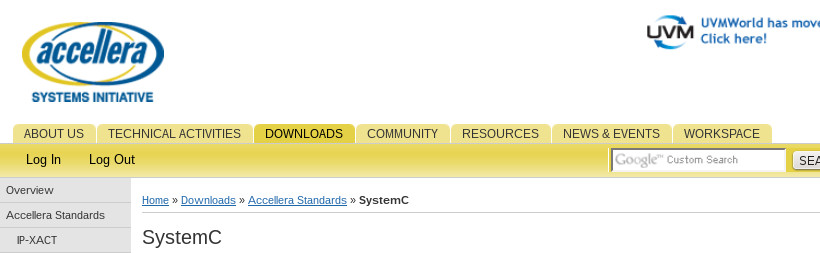
\includegraphics[width=0.6\textwidth]{introduction/figures/osci_homepage.jpg}
		\end{itemize}
		\item<1-> To download SystemC you will have to register yourself into the Accellera website.
		\item<1-> From the same site you can download:
		\begin{itemize}
			\item<1-> reference manuals and documents,
			\item<1-> new SystemC proposals and standards.
		\end{itemize}
	\end{itemize}
\end{frame}

\begin{frame}
	\frametitle{Installing Accellera SystemC\newline Compile \& Install}
	\begin{itemize}
		\item<1-> Uncompress the downloaded file.
		\item<1-> Create a directory for the compilation and a directory to install the final library.
		\item<1-> Into the compilation directory perform the typical \texttt{configure}, \texttt{make} and \texttt{make install} to install the SystemC library.
	\end{itemize}
	\lstinputlisting[language= ,basicstyle=\ttfamily\tiny,numbers=none,breaklines=true,framexleftmargin=0.5mm,xleftmargin=0.06\textwidth,xrightmargin=0.06\textwidth]{introduction/install.txt}
\end{frame}
}

\mode<article>{
To install SystemC you will have to download it from the Accellera SystemC site: \url{http://www.systemc.org}~.
To do so you will have to register yourself into the Accellera site.
From the same site you can download other documents, manuals and the new proposals like the TLM2.0 proposal.

Once you have downloaded the SystemC compressed file you have to simply uncompress it and follow the indications that appear in the INSTALL file.
Those instructions will depend on the operating system you use.
Currently SystemC can be install under Windows, Linux and MacOSX among others.

Under Linux you will have to create a directory were SystemC will be compiled (we will call it \texttt{obj} for our example). 
From the \texttt{obj} directory you will have to call the \texttt{configure} script available from the downloaded SystemC distribution (see Figure~\ref{technically_systemc_configure}). 
The \texttt{configure} script accepts different options but usually you will be only using the \texttt{--prefix} option, which defines in which directory the SystemC library will be installed.
Note that the installation directory needs to be created before performing the following step.
Once the \texttt{configure} script has finished its task, you can perform the typical\footnote{At least typical for  many Linux users.} \texttt{make} and \texttt{make install} to compile and install the SystemC library\footnote{If you selected as install directory a directory that belongs to another user, for example the root user, you will have to perform the \texttt{make install} step under that user.}.

\begin{figure}[!h]
\begin{center}
		\lstinputlisting[language= ,basicstyle=\ttfamily\normalsize,numbers=none,breaklines=true,framexleftmargin=0.5mm,xleftmargin=0.06\textwidth,xrightmargin=0.06\textwidth]{introduction/install.txt}
\end{center}
\caption{Commands to install SystemC (example).}
\label{technically_systemc_configure}
\end{figure}

Now you can develop simulators based on SystemC using your newly installed library.
When creating your simulators you will have to include the \texttt{systemc.h} header file that you can find in the \texttt{include} directory of your installation. 
When compiling you will have to define the location of the SystemC headers directory and precise that you are using the SystemC library and its location (the \texttt{lib-linux} directory).
}


% \section{Conclusion}
\label{sec:conclusion}

This document has presented the different tests that have been performed in order to validate the ARM7TDMI simulator.
With the SPEC2000 application suit the simulator have been validated to be used with real world applications.
Thanks to the random tests technique developped at CEA an extensive validation of all the ARM7TDMI user level instructions have been done.
Finally, with the development of a small kernel the simulator has been validated for the execution of system level applications, like operating systems, drivers, and embedded applications.

As for any software application, the validation does not ensure that the simulator is bug free.
However, the validation performed ensures that the simulator functionality matches the ARM7TDMI functionality, and that any application can be run on it with confidence.
Additionally, the ARM7TDMI simulator provided in UNISIM (\url{http://www.unisim.org}) is open source, which means that users can fixe it if necessary and that corrections to the simulator can be easily shared.




\newpage

\mode<article>{
\chapter{SystemC TLM 2.0}
}

\mode<presentation>{
\part{SystemC TLM 2.0}
}

\mode<presentation>{
\begin{frame}
	\frametitle{VP4: SystemC TLM 2.0}
	\begin{block}{Accelera SystemC TLM 2.0}
		The Transaction Level Modeling standard of Accelera (previously the Open SystemC Initiative - OSCI).
	\end{block}
	\begin{itemize}
		\item<1-> Introduction
		\item<1-> Interfaces
		\item<1-> Sockets
		\item<1-> Temporal decoupling and the Quantum Keeper
		\item<1-> The Generic Payload
	\end{itemize}
\end{frame}
}

\subsection {Eléments de contexte}
Au cours de mon cursus à l'Ecole d'ingénieur Denis Diderot, j'ai eu l'occasion d'effectuer un stage de 6 mois entre la 2 ième et 3 ième année. 
J'ai donc choisi d'effectuer ce stage au C.E.A List afin d'avoir une expérience professionelle dans un organisme de recherche en informatique et de développer de nouvelles connaissances dans le domaine des systèmes embarqués.
Ma formation étant spécialisé dans la conception de logiciels embarqués et ayant suivi des cours d'architecture des processeurs, 
j'ai pensé qu'il serai intéressant d'approfondir mes connaissances dans le fonctionnenent des processeur afin d'avoir une vision plus complète de l'éxecution des programmes (niveau assembleur).
Gilles Mouchard et Reda Nouacer de l'équipe UNISIM recherchaient un étudiant afin d'effectuer un stage de 6 mois consistant à réaliser un simulateur de jeu d'instruction (ISS) d'un proceseur embarqué. 
\subsection{Contenue du document}
Ce document décrit le travail réalisé au cours de ce stage pendant la période du 10 mars au 31 août 2014 au sein du laboratoire LSL du CEA LIST.
Après une brève présentation du laboratoire et de l'équipe, j'établirai un  état de l'art sur les méthodes de conception et validation d'un simulateur suivie la présentation des outils utilisés pour le projet.
Puis je décrirai les étapes de réalisation et les résulats obtenues sur le processeur choisie par l'équipe.
J'évoquerai également les problèmes rencontrés et les moyens pour les résoudre. 
Enfin j'établirai un bilan sur les connaissances acquises durant ce stage concernant la simulation mais aussi plus généralement sur les méthodes de développement de logiciel.      

\mode<article>{
	\clearpage
}

\section{Interfaces}

\mode<presentation>{
\begin{frame}
	\frametitle{Core TLM2 interfaces}
	\begin{block}{Definition}
		An interface is the way modules use to communicate between each
		other.
	\end{block}
	\begin{itemize}
		\item<1-> TLM2 keeps the core interfaces from TLM1.
		\item<1-> TLM2 adds the following interfaces:
		\begin{itemize}
			\item<1-> blocking and non-blocking transport interfaces,
			\item<1-> a direct memory interface (DMI), and
			\item<1-> a debug transaction interface.
		\end{itemize}
	\end{itemize}
\end{frame}
}

\mode<article>{
As we have seen for Cycle Level Modeling modules used ports to communicate with each other.
With Transaction Level Modeling modules still use ports, however they are quite different.
Ports under TLM are attached to interfaces, those are methods that are implemented by the target module.
TLM2 defines a series of interfaces that the programmer can use to implement his/her TLM simulator.

TLM2 for compatibility issues kept the interfaces defined by TLM1, so previous simulators using TLM1 interfaces could be used with the new TLM definition.
However, the TLM Accellera working group recommends to build new modules using TLM2 interfaces and writing rules.
For this reason we are not going to explain TLM1 interfaces and focus only on the new TLM2 interfaces.

In the following subsections the TLM2 interfaces will be introduced in detail:
\begin{itemize}
	\item the blocking transport interface,
	\item the non-blocking transport interface,
	\item the direct memory interface (DMI), and
	\item the debug transaction interface.
\end{itemize}
}

\subsection{Blocking transport interface}

\mode<presentation>{
\begin{frame}
	\frametitle{Blocking transport interface}
	\setbeamercolor{postit}{fg=black,bg=yellow}
	\begin{beamercolorbox}[center,rounded=true,wd=\textwidth]{postit}
		Designed for the untimed and loosely-timed coding style.
	\end{beamercolorbox}
	\begin{itemize}
		\item<1->Definition:
	\begin{figure}[h]
		\lstinputlisting{tlm/b_transport.cc}
	\end{figure}
		\item<2->The \texttt\textbf{TRANS} argument is by default set to \texttt{\textbf{tlm\_generic\_payload}}.
		\item<3->Recommended to use the generic payload for interoperability issues.
		\item<4->\texttt{sc\_time} parameter: precise simulation time (relative to the last synchronization) the call is taking place.
	\end{itemize}
\end{frame}

\begin{frame}
	\frametitle{Blocking transport interface: Rules (I)}
	\begin{enumerate}
	\item The caller is responsible for allocating storage and for constructing the transaction object. 
	The \texttt{\textbf{b\_transport}} method shall be called with a fully initialized transaction object.
	\item In the case of the generic payload, the call to \texttt{\textbf{b\_transport}} shall mark the first timing point of the transaction.
	The return from \texttt{\textbf{b\_transport}} shall mark the final timing point of the transaction.
	\item The callee may modify or update both the transaction object or the time. Modifications of the transaction object is subject to any constraints imposed by the transaction class \texttt{\textbf{TRANS}}.
	\item The caller is responsible for deleting or pooling the transaction object after the call.
	\end{enumerate}
\end{frame}

\begin{frame}
	\frametitle{Blocking transport interface: Rules (II)}
	\begin{enumerate}
	\item The callee shall assume that the caller will invalidate the transaction object upon return from \texttt{\textbf{b\_transport}}.
	\item The \texttt{\textbf{b\_transport}} method supports temporal decoupling.
	\item It is recommended that the transaction object should not contain timing information. 
	\item \texttt{\textbf{b\_transport}} may make one or several calls to \texttt{\textbf{nb\_transport\_fw}}. 
	It is straightforward to create an adapter between an untimed or loosely-timed initiator and an approximately-timed target.
	\end{enumerate}
\end{frame}
}

\mode<article>{
The TLM2 blocking interface supports an untimed and loosely-timed modeling style.
It defines the \texttt{\textbf{b\_transport}} method, which takes two non-const reference arguments, used by the source module to set the message and emission time and by the target module to set the response and update time. 
Figure~\ref{fig:b_transport_definition} shows the blocking interface definition.
\begin{figure}[h]
	\lstinputlisting{tlm/b_transport.cc}
	\caption{The blocking transport interface class definition.}
	\label{fig:b_transport_definition}
\end{figure}

\subsubsection{The \texttt{TRANS} template argument}
The purpose of this interface (and of the non-blocking interfaces that we will see later) is to make possible transport transactions of any type.
However, for a maximum interoperability between modules of different constructors a default transaction type is proposed: the \texttt{\textbf{tlm\_generic\_payload}}.

Applications should use the default transaction type \texttt{\textbf{tlm\_generic\_payload}} or extend it if needed. 
We will see the specifics of the generic payload and how it can be extended later in this chapter.

The initiator is responsible for the allocation of the transaction object and its destruction once the response has been received.
The target module can only use the received transaction object during the call of the \texttt{\textbf{b\_transport}}, after that it must suppose that the transaction object no longer exists.

\subsubsection{Rules}
When using the blocking transport interface the following rules must be followed:
\begin{enumerate}
	\item The caller is responsible for allocating storage and for constructing the transaction object. 
	The \texttt{\textbf{b\_transport}} method shall be called with a fully initialized transaction object.
	\item In the case of the generic payload, the call to \texttt{\textbf{b\_transport}} shall mark the first timing point of the transaction.
	The return from \texttt{\textbf{b\_transport}} shall mark the final timing point of the transaction.
	\item The callee may modify or update the transaction object, subject to any constraints imposed by the transaction class \texttt{\textbf{TRANS}}.
	\item The caller is responsible for deleting or pooling the transaction object after the call.
	\item The callee shall assume that the caller will invalidate the transaction object upon return from \texttt{\textbf{b\_transport}}.
	\item The \texttt{\textbf{b\_transport}} method supports temporal decoupling.
	\item It is recommended that the transaction object should not contain timing information. 
	\item \texttt{\textbf{b\_transport}} may make one or several calls to \texttt{\textbf{nb\_transport\_fw}}. 
	It is straightforward to create an adapter between an untimed or a loosely-timed initiator and an approximately-timed target.
\end{enumerate}
}

\subsection{Non-blocking transport interfaces}

\mode<presentation>{
\begin{frame}
	\frametitle{Non-blocking transport interfaces}
	\setbeamercolor{postit}{fg=black,bg=yellow}
	\begin{beamercolorbox}[center,rounded=true,wd=\textwidth]{postit}
		Designed for the approximately-timed coding style.
	\end{beamercolorbox}
	\begin{figure}[h]
		\lstinputlisting{tlm/nb_transport.cc}
	\end{figure}
\end{frame}

\begin{frame}
	\frametitle{Non-blocking transport interfaces (II)}
	\begin{itemize}
		\item Must be defined by both initiator and target.
		\begin{center}
			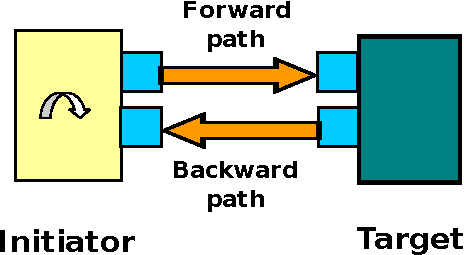
\includegraphics[width=0.6\textwidth]{tlm/figures/nb_fig.pdf}
		\end{center}
		\item Parameters and return value:
		\begin{itemize}
			\item The transaction (\texttt{tlm\_generic\_payload}).
			\item \texttt{\textbf{PHASE}} indicates the state of the transaction: \texttt{\textbf{BEGIN\_REQ}}, \texttt{\textbf{END\_REQ}}, \texttt{\textbf{BEGIN\_RESP}}, and \texttt{\textbf{END\_RESP}}.
			\item The \texttt{sc\_time} parameter indicates the precise simulation time (relative to the last synchronization) the call is taking place.
			\item The return value (\texttt{tlm\_sync\_enum}) indicates the  call status, and fixes synchronization points.
		\end{itemize}
	\end{itemize}
\end{frame}

\begin{frame}
	\frametitle{Non-blocking transport interfaces: Rules (I)}
	\begin{enumerate}
		\item The \texttt{\textbf{nb\_transport\_fw}} and \texttt{\textbf{nb\_transport\_bw}} methods shall not call wait, directly or indirectly.
		\item The \texttt{\textbf{nb\_transport\_fw}} and \texttt{\textbf{nb\_transport\_bw}} methods may be called from a thread process or from a method process.
		\item With the approximately-timed coding style, \texttt{\textbf{nb\_transport\_fw}} and \texttt{\textbf{nb\_transport\_bw}} are called respectively along the forward and backward paths between initiator and target.
		In the case of the generic payload, the two paths should pass through exactly the same sequence of components and sockets, obviously in reverse order.
	\end{enumerate}
\end{frame}

\begin{frame}
	\frametitle{Non-blocking transport interfaces: Rules (II)}
	\begin{enumerate}
		\item The initiator is responsible for deleting or pooling the transaction object after the final timing point. 
		\item If an interconnect component or a target needs to access the state of the transaction after the final call to \texttt{\textbf{nb\_transport\_fw}} or \texttt{\textbf{nb\_transport\_bw}} for a particular transaction instance, it must make a copy of the transaction object.
		\item A \texttt{\textbf{nb\_transport\_fw}} call on the forward path shall under no circumstances directly or indirectly make a call to \texttt{\textbf{nb\_transport\_bw}} on the associated backward path, and vice versa.
	\end{enumerate}
\end{frame}

\begin{frame}
	\frametitle{\small Non-blocking transport interfaces: The \texttt{phase} argument}
	\vspace{0.4em}
	\setbeamercolor{postit}{fg=black,bg=yellow}
	\begin{beamercolorbox}[center,rounded=true,wd=\textwidth]{postit}
		It serves to program protocols phases.
	\end{beamercolorbox}
	\begin{itemize}
		\item<1-> Both caller and callee can modify its value.
		\item The \texttt{tlm\_phase} enum defines four different phase status:
		\begin{itemize}
			\item<1-> \texttt{BEGIN\_REQ}
			\item<1-> \texttt{END\_REQ}
			\item<1-> \texttt{BEGIN\_RESP}
			\item<1-> \texttt{END\_RESP}
		\end{itemize}
	\end{itemize}
	\onslide<2->
	\vspace{-0.9em}
	\begin{center}{
	\scriptsize
	\begin{tabular}{|l|l|l|}
		\hline
		\texttt{\textbf{tlm\_phase}} & \textbf{Coding style} & \textbf{Path} \\
		\hline
		\texttt{BEGIN\_REQ} & Loosely- and approximately-timed & Forward(call) \\
		\hline
		\texttt{END\_REQ} & Approximately-timed only & Forward(return) \\
		& & Backward(call) \\
		\hline
		\texttt{BEGIN\_RESP} & Loosely- and approximately-timed & Forward(return) \\
		& & Backward(call) \\
		\hline
		\texttt{END\_RESP} & Approximately-timed only & Forward(call) \\
		& & Backward(return) \\
		\hline
	\end{tabular}
	}
	\end{center}
\end{frame}

\begin{frame}
	\frametitle{\small Non-blocking transport interface: The \texttt{sc\_time} argument}
	\setbeamercolor{postit}{fg=black,bg=yellow}
	\begin{beamercolorbox}[center,rounded=true,wd=\textwidth]{postit}
		It is used to indicate when the current transaction phase is taking place.
	\end{beamercolorbox}
	\begin{itemize}
		\item<1-> It is always a positive number.
		\item<1-> It is relative to the current simulation time, as returned from \texttt{sc\_time\_stamp}.
	\end{itemize}
	\onslide<2->
	\begin{block}{Temporal decoupling}
		Thanks to this argument the simulators can implement \emph{temporal decoupling}, that is running without yielding control (calling \texttt{wait(\ldots)}) to the SystemC scheduler.
		\newline \newline
		\emph{This enhances the performance of the simulator.}
	\end{block}
\end{frame}

\begin{frame}
	\frametitle{\small Non-blocking transport interface: \texttt{tlm\_sync\_enum} return arg.}
	\setbeamercolor{postit}{fg=black,bg=yellow}
	\begin{beamercolorbox}[center,rounded=true,wd=\textwidth]{postit}
		It signals if the call was a success or something failed, and if a synchronization is needed.
	\end{beamercolorbox}
	Four possible values:
	{\footnotesize
	\definecolor{MyDarkGreen}{rgb}{0,0.45,0}
	\newcommand{\X}{\textbf{\color{MyDarkGreen}$\surd$}}
	\newline
	\begin{tabular}{|l|p{2.5em}|p{2.5em}|l|l|}
		\hline
		\texttt{\textbf{tlm\_sync\_enum}} & \multicolumn{2}{l|}{\textbf{Coding style}} & \textbf{Transaction and} & \textbf{Timing} \\
		\cline{2-3}
		& {\protect \centering LT} & {\protect \centering AT} & \textbf{phase arguments} & \textbf{annotation} \\
		\hline
		\texttt{TLM\_ACCEPTED} & \X & \X & Unmodified &  \\
		\hline
		\texttt{TLM\_UPDATED} & & \X & Updated & \X \\
		\hline
		\texttt{TLM\_COMPLETED} & \X & \X & Updated\tiny{(but caller} & \X \\
		& & & \tiny{may ignore phase)} & \\
		\hline
	\end{tabular}
	}
\end{frame}
}

\mode<article>{
The non-blocking transport interfaces exist to support the loosely-timed and approxitemately-timed coding styles.
Figure~\ref{fig:nb_transport_definition} shows the non-blocking transport interfaces definitions.

\begin{figure}[h]
	\lstinputlisting{tlm/nb_transport.cc}
	\caption{The non-blocking transport interfaces class definitions.}
	\label{fig:nb_transport_definition}
\end{figure}

The non-blocking transport interfaces defines the \texttt{\textbf{nb\_transport\_fw}} and \texttt{\textbf{nb\_transport\_bw}} methods which, as the blocking transport interface method \texttt{\textbf{b\_transport}}, passes a non-const reference to the transaction object.
The \texttt{\textbf{nb\_transport\_fw}} and \texttt{\textbf{nb\_transport\_bw}} methods also passe two other parameters:
\begin{itemize}
	\item a non-const reference to a \texttt{\textbf{PHASE}} object to indicate the state of the transaction, and
	\item a time to annotate the delay of the next phase transition.
\end{itemize}
Additionally the \texttt{\textbf{nb\_transport\_fw}} and \texttt{\textbf{nb\_transport\_bw}} methods can return a value (\texttt{\textbf{tlm\_sync\_enum}}) to indicate the status of the call, and signal synchronization points. 

Unlike the blocking transport interface, the non-blocking transport interfaces needs to be defined by both, the initiator and the target modules.
That is, there is a forward non-blocking transport interface used by the initiator to send requests and a backward non-blocking transport interface used by the target to send the responses.

\subsubsection{Rules}
When using the non-blocking transport interface the following rules must be followed:
\begin{enumerate}
	\item The \texttt{\textbf{nb\_transport\_fw}} and \texttt{\textbf{nb\_transport\_bw}} methods shall not call wait, directly or indirectly.
	\item The \texttt{\textbf{nb\_transport\_fw}} and \texttt{\textbf{nb\_transport\_bw}} methods may be called from a thread process or from a method process.
	\item Exceptionally, if both the blocking and non-blocking transport interfaces are being used together, \texttt{\textbf{nb\_transport\_fw}} may need to call \texttt{\textbf{b\_transport}}. 
	This is only technically possible if it can be guaranteed that the \texttt{\textbf{b\_transport}} method does not call wait, directly or indirectly, but is in any case bad practice.
	Otherwise, the solution is to call to \texttt{\textbf{b\_transport}} from a separate thread process, spawned or notified by the original \texttt{\textbf{nb\_transport\_fw}} call.
	\item With the approximately-timed coding style, \texttt{\textbf{nb\_transport\_fw}} and \texttt{\textbf{nb\_transport\_bw}} mathod are called respectively along the forward and backward paths between initiator and target. 
	In the case of the generic payload, the two paths should pass through exactly the same sequence of components and sockets, obviously in reverse order.
	\item The initiator is responsible for deleting or pooling the transaction object after the final timing point. 
	The final timing point may be marked by a call to or a return from either \texttt{\textbf{nb\_transport\_fw}} on the forward path or \texttt{\textbf{nb\_transport\_bw}} on the backward path. 
	If the final call to non-blocking transport interfaces is on the forward path (i.e. \texttt{\textbf{nb\_transport\_fw}}), the initiator may delete the transaction object on return from \texttt{\textbf{nb\_transport\_fw}}.
	If the final call to non-blocking transport interface is on the backward path (i.e. \texttt{\textbf{nb\_transport\_bw}} , the initiator may delete the transaction object the next time the initiator process resumes, in which case the transaction object shall remain valid and accessible by the target until the target yields to the SystemC scheduler. 
	In other words, if the final call to non-blocking transport interfaces is from target to initiator, the target has a chance to inspect the state of the transaction object before it yields control. 
	After that, any interconnect component or target must assume that the transaction object is invalid.
	\item If an interconnect component or a target needs to access the state of the transaction after the final call to non-blocking transport interfaces for a particular transaction instance, it must make a copy of the transaction object.
	\item A call to non-blocking transport interfaces on the forward path shall under no circumstances directly or indirectly make a call to non-blocking transport interfaces on the associated backward path, and vice versa.
\end{enumerate}

\subsubsection{The \texttt{TRANS} template argument}
The same rules that apply to the transport blocking interface are applied to the non-blocking interface.
However, it must be noted that the life of the transaction expands from the forward request from the initiator starting the request to the backward response from the target module.

\subsubsection{The \texttt{phase} argument}
The phase argument serves to program protocols phases.
The generic payload uses the specific enum \texttt{\textbf{tlm\_phase}}.
Other protocols may substitute it with their own phase types, but this will imply a loss of interoperability.

The \texttt{\textbf{phase}} argument is passed as a non-const reference, which means that both the caller and the callee can change its value.

The \texttt{\textbf{tlm\_phase}} enum defines four different phase status:
\begin{itemize}
	\item \texttt{\textbf{BEGIN\_REQ}}: it marks the beginning of the transaction request.
	It can be used by the approximately-timed coding style.
	The initiator uses this phase when starting a non-blocking transport transaction.
	\item \texttt{\textbf{END\_REQ}}: it marks the end of the transaction request.
	It is only used for the approximately-timed coding style.
	The target uses this phase when finishing a non-blocking transport transaction.
	\item \texttt{\textbf{BEGIN\_RESP}}: it is used by the callee to mark the beginning of the transaction response.
	It can be used by the approximately-timed coding style.
	The transaction callee module can start the response at different points, for example setting the forward call phase argument when returning from a \texttt{\textbf{BEGIN\_REQ}} or \texttt{\textbf{END\_REQ}}, or initiating a backward call.
	\item \texttt{\textbf{END\_RESP}}: it marks the end of the transaction response.
	It is only used for the approximately-timed coding style.
	The initiator uses this phase when finishing a non-blocking transport transaction.
\end{itemize}
Table~\ref{table:tlm_phase_values} summarizes the usage of the \texttt{\textbf{tlm\_phase}} values across the coding styles.
The different values of the phase are used in cycles, but the initiator and target can remove steps if necessary (specially in the case of approximately-timed coding style).
Each time a \texttt{\textbf{BEGIN\_REQ}} is sent a new transaction starts.
Figure~\ref{fig:tlm_phase_sequences} shows the possible phase sequences (note however that these sequences must be used in accordance with the \texttt{tlm\_sync\_enum} return argument).
In section \emph{Loosely-timed coding style} and \emph{Approximately-timed coding style} the different phase values will be explained with examples.

\begin{table}[h]
	\begin{center}
	\begin{tabular}{|l|l|l|}
		\hline
		\texttt{\textbf{tlm\_phase}} & \textbf{Coding style} & \textbf{Path} \\
		\hline
		\texttt{BEGIN\_REQ} & Loosely- and approximately-timed & Forward(call) \\
		\hline
		\texttt{END\_REQ} & Approximately-timed only & Forward(return) Backward(call) \\
		\hline
		\texttt{BEGIN\_RESP} & Loosely- and approximately-timed & Forward(return) Backward(call) \\
		\hline
		\texttt{END\_RESP} & Approximately-timed only & Forward(call) Backward(return) \\
		\hline
	\end{tabular}
	\end{center}
	\caption{Usage of the \texttt{tlm\_phase} values across the coding styles.}
	\label{table:tlm_phase_values}
\end{table}


\begin{figure}[h]
	\begin{center}
\begin{tabular}{|l|}
\hline
\texttt{BEGIN\_REQ} {\footnotesize($\to$ \texttt{BEGIN\_RESP})}\\
\texttt{BEGIN\_REQ} $\to$ \texttt{BEGIN\_RESP}\\
\texttt{BEGIN\_REQ} $\to$ \texttt{END\_REQ} {\footnotesize($\to$ \texttt{BEGIN\_RESP} $\to$ \texttt{END\_RESP})}\\
\texttt{BEGIN\_REQ} $\to$ \texttt{END\_REQ} $\to$ \texttt{BEGIN\_RESP} {\footnotesize($\to$ \texttt{END\_RESP})}\\
\texttt{BEGIN\_REQ} {\small($\to$ \texttt{END\_REQ})} $\to$ \texttt{BEGIN\_RESP} $\to$ \texttt{END\_RESP}\\
\texttt{BEGIN\_REQ} $\to$ \texttt{END\_REQ} $\to$ \texttt{BEGIN\_RESP} $\to$ \texttt{END\_RESP}\\
\hline
\end{tabular}
	\end{center}
	\caption{Permitted phase transition sequences.}
	\label{fig:tlm_phase_sequences}
\end{figure}

\subsubsection{The \texttt{sc\_time} argument}
The \texttt{sc\_time} argument is used to indicate when the current transaction phase is taking place.
It is always a positive number and it is relative to the current simulation time (as the time you can get from \texttt{sc\_time\_stamp()} call). 
So for example if an initiator module calls \texttt{nb\_transport\_fw} it can use the \texttt{sc\_time} argument to indicate the time at which the call is made, without having to do a wait to synchronize itself with the SystemC scheduler.

Thanks to this argument the simulators can implement what is called \emph{temporal decoupling}, that is running without yielding control to the SystemC scheduler.
Avoiding yields to the SystemC scheduler enhances the performance of the simulator.
However it is important to note that it is the responsibility of the simulator writer to handle temporal decoupling.

\subsubsection{The \texttt{tlm\_sync\_enum} return argument}
Once the callee has processed the \texttt{nb\_transport\_fw} or \texttt{nb\_transport\_bw} call it must return the status of the call, signaling if it was a success or something failed, and if a synchronization is needed.
The TLM 2.0 proposes four different status responses:
\begin{itemize}
	\item \texttt{\textbf{TLM\_ACCEPTED}}: The callee accepts the transaction, and the transaction state or time argument should not have been modified during the call.
	The caller should not take further actions on the transaction, and wait for the response from the callee.
	Following the call to \texttt{nb\_transport\_fw} or \texttt{nb\_transport\_bw} the caller should synchronize, this is know as synchronization-on-demand.
	This response is used by the approximately-time coding style.
	\item \texttt{\textbf{TLM\_UPDATED}}: The callee has accepted and updated the transaction, but the transaction has not been completed.
	The callee should have modified the state of the transaction object and the phase argument during the call, and the time argument may have been updated.
	Following the call to \texttt{nb\_transport\_fw} or \texttt{nb\_transport\_bw} the caller should synchronize (synchronization-on-demand).
	This response is used only on approximately-timed coding style.
	\item \texttt{\textbf{TLM\_COMPLETED}}: The transaction has been accepted and completed.
	The caller, after the call to \texttt{nb\_transport\_fw} or \texttt{nb\_transport\_bw} can inspect the contents of the transaction object and the time argument.
	Additionally, the caller can ignore the phase argument because the transaction has been completed.
	There should not be further actions on this transaction once it has been completed.
	This response is used by the approximately-time coding style.
\end{itemize}
Table~\ref{table:tlm_sync_enum_values} summarizes the usage of the \texttt{\textbf{tlm\_phase}} values across the coding styles.

\begin{table}[h]
	\begin{center}
	\begin{tabular}{|l|l|l|l|}
		\hline
		\texttt{\textbf{tlm\_sync\_enum}} & \textbf{Coding style} & \textbf{Transaction and} & \textbf{Timing} \\
		&  & \textbf{phase arguments} & \textbf{annotation} \\
		\hline
		\texttt{TLM\_ACCEPTED} & Loosely- and approximately-timed & Unmodified & No \\
		\hline
		\texttt{TLM\_UPDATED} & Approximately-timed only & Updated & Yes \\
		\hline
		\texttt{TLM\_COMPLETED} & Loosely- and approximately-timed & Updated, but caller & Yes \\
		& & may ignore phase & \\
		\hline
	\end{tabular}
	\end{center}
	\caption{Usage of the \texttt{tlm\_sync\_enum} values across the coding styles.}
	\label{table:tlm_sync_enum_values}
\end{table}

}

\subsection{Direct memory interface}

\mode<presentation>{

\begin{frame}
	\frametitle{DMI: Direct Memory Interface}
	\begin{block}{}
		This interface provides direct access to an area of memory owned by a target.\\
		It bypasses the usual path through the interconnect components used by the transport interface.\\
	\end{block}
	\begin{itemize}
		\item<1-> Intended to {\color{red}accelerate} regular memory transactions in an untimed or loosely-timed simulation.
		\item<1-> DMI is composed by two basic interfaces that must be always be used in conjunction:
		\begin{itemize}
			\item<1-> \texttt{tlm\_fw\_direct\_mem\_if}
			\item<1-> \texttt{tlm\_bw\_direct\_mem\_if}
		\end{itemize}
	\end{itemize}
\end{frame}
}

\mode<article>{
The direct memory interface (DMI) is a specialized interface distinct from the transport interface, providing direct access to an area of memory owned by a target. 
The DMI interface bypass the usual path through the interconnect components used by the transport interface.
DMI is intended to accelerate regular memory transactions in an untimed or loosely-timed simulation.

In this document we will not study this interface in detail.
However you need to know that it exists and its definition because as we will later see it is indirectly used by the classes you will be using when making TLM 2.0 based simulators.

Figure~\ref{fig:tlm_dmi_definition} shows the \texttt{tlm\_dmi} class definition.
DMI is composed of two basic interfaces that must be always be used in conjunction:
\begin{itemize}
	\item \texttt{tlm\_fw\_direct\_mem\_if}: this interface is used by the initiator module to request the target module for a pointer to a memory zone.
	\item \texttt{tlm\_bw\_direct\_mem\_if}: this interface is used by the target module to request the initiator module to invalidate the pointer to a memory zone that was previously provided.
	If the initiator wants to use again the direct access to the memory zone, it must request the memory zone again using the \texttt{tlm\_fw\_direct\_mem\_if}.
\end{itemize}

\begin{figure}[!h]
	\lstinputlisting{tlm/tlm_dmi.hh}
	\caption{The direct memory interfaces class definitions.}
	\label{fig:tlm_dmi_definition}
\end{figure}

In this tutorial we will not be using those interfaces, but we will need to provide an implementation for those interfaces.
The implementation of \texttt{tlm\_fw\_direct\_mem\_if} (done by the target module) should return a \texttt{false}, which indicates to the initiator target that it can not provide a pointer to the memory zone requested.
The implementation of \texttt{tlm\_bw\_direct\_mem\_if} (done by the initiator module) does not need to do anything, because as you will not be requesting the target modules for a pointer to a memory zone, no pointers will need to be invalidated.
However you may add to its implementation an error message to check that your target modules never call this method.
}

\subsection{Debug transaction interface}

\mode<presentation>{

\begin{frame}
	\frametitle{Debug transaction interface}
	\begin{block}{}
		The debug transaction interface provides debug access to an area of memory owned by a target.
	\end{block}
	\begin{itemize}
		\item<1-> It is for debug access free of the delays or side-effects associated with regular transactions.
		\item<1-> It provides a single forward interface:
		\begin{itemize}
			\item<1-> \texttt{tlm\_transport\_dbg\_if}
		\end{itemize}
	\end{itemize}
\end{frame}
}

\mode<article>{
The debug transaction interface is a specialized interface distinct from the transport interface, providing debug access to an area of memory owned by a target. 
The debug transaction interface bypasses the usual path through the interconnect components used by the transport interface. 
The debug transaction interface is for debug access free of the delays or side-effects associated with regular transactions.\footnote{For those of you who know UNISIM-VP, this interface is very close (not to say identical) to the non-intrusive memory interface used by the UNISIM-VP simulators.}

As for the DMI interface, we will not study this interface in detail, however we will briefly present it. 
Figure~\ref{fig:tlm_transport_dbg_if_definition} shows the debug transport interface class definition.
It defines a single forward interface: \texttt{tlm\_transport\_dbg\_if}.
This interface is used by the initiator to access to a memory zone of the target module non-intrusively.

\begin{figure}[!h]
	\lstinputlisting{tlm/tlm_transport_dbg_if.hh}
	\caption{The debug transaction interface class definition.}
	\label{fig:tlm_transport_dbg_if_definition}
\end{figure}

You will need to provide an implementation of this interface on your target modules.
As we will not be using it, you can simply return a \texttt{0} value, which means that your target module can not provide the data requested by the initiator module.
}


\mode<article>{
	\clearpage
}

\section{Sockets and combined interfaces}

\mode<presentation>{
\begin{frame}
	\frametitle{Sockets and combined interfaces}
	A \emph{socket} is a facility class that combines an export with a port.
	Two different sockets:
	\begin{itemize}
		\item<1-> \textbf{initiator}:
		\begin{itemize}
			\item<1-> port for the forward path
			\item<1-> export for the backward path
		\end{itemize}
		\item<1-> \textbf{target}:
		\begin{itemize}
			\item<1-> export for the forward path
			\item<1-> port for the backward path
		\end{itemize}
	\end{itemize}
	\begin{center}
		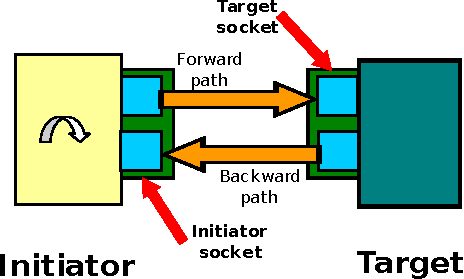
\includegraphics[width=0.6\textwidth]{tlm/figures/socket_fig.pdf}
	\end{center}
\end{frame}

\begin{frame}
	\frametitle{Sockets benefits}
	\begin{itemize}
		\item<1-> They group the transport, direct memory and debug transaction interfaces for both the forward and backward paths together into a single object.
		\item<1-> They provide methods to bind port and export of both the forward and backward paths in a single call.
		\item<1-> They offer strong type checking when binding sockets parameterized with incompatible protocol types.
		\item<1-> They include a bus width parameter that may be used to interpret the transaction.
	\end{itemize}
\end{frame}

\begin{frame}
	\frametitle{Initiator socket definition}
	\lstinputlisting{tlm/tlm_socket_initiator.hh}
\end{frame}

\begin{frame}
	\frametitle{Target socket definition}
	\lstinputlisting{tlm/tlm_socket_target.hh}
\end{frame}

\begin{frame}
	\frametitle{Combined interfaces}
	\lstinputlisting{tlm/combined_interfaces.hh}
\end{frame}

\begin{frame}
	\frametitle{The \texttt{tlm\_generic\_payload\_types}}
	\lstinputlisting{tlm/tlm_socket_types.hh}
\end{frame}
}
\mode<article>{
TLM 2.0 introduced a new facility: the \emph{sockets}.
Sockets are just classes that facilitate the writing of modules using the guidelines proposed by the TLM 2.0 working group.
Two different sockets types are provided: the \emph{initiator} and \emph{target sockets}.
A socket combines a port with and export.
An initiator socket has a port for the forward path and an export for the backward path, whilst a target socket has an export for the forward path and a port for the backward path.
Figures~\ref{fig:tlm_socket_initiator} and ~\ref{fig:tlm_socket_target} show the class definitions for the initiator and the target socket respectively.

\begin{figure}[h]
	\lstinputlisting{tlm/tlm_socket_initiator.hh}
	\caption{The basic initiator socket class definition.}
	\label{fig:tlm_socket_initiator}
\end{figure}

\begin{figure}[h]
	\lstinputlisting{tlm/tlm_socket_target.hh}
	\caption{The basic target socket class definition.}
	\label{fig:tlm_socket_target}
\end{figure}

Sockets use combined interfaces, that is groups of TLM 2.0 interfaces. 
Those combined interfaces include not only transport interfaces, but direct memory and debug transaction interfaces.
Four different combined interfaces exist, combining forward and backward interfaces with blocking and non-blocking transport interfaces.
Figure~\ref{fig:combined_interfaces} shows the class definitions for the four combined interfaces:
\begin{itemize}
	\item blocking transport (identified by the \texttt{\_b\_} infix):
	\begin{itemize}
		\item forward interface (identified by the \texttt{\_fw\_} infix): \texttt{tlm\_fw\_b\_transport\_if}
		\item backware interface (identified by the \texttt{\_bw\_} infix): \texttt{tlm\_bw\_b\_transport\_if}
	\end{itemize}
	\item non-blocking transport (identified by the \texttt{\_nb\_} infix):
	\begin{itemize}
		\item forward interface (identified by the \texttt{\_fw\_} infix): \texttt{tlm\_fw\_nb\_transport\_if}
		\item backware interface (identified by the \texttt{\_bw\_} infix): \texttt{tlm\_bw\_nb\_transport\_if}
	\end{itemize}
\end{itemize}

\begin{figure}[h]
	\lstinputlisting{tlm/combined_interfaces.hh}
	\caption{The four basic combined interfaces class definitions.}
	\label{fig:combined_interfaces}
\end{figure}

The four combined interfaces are parametrized by a single \emph{protocol types class} which defines the different protocols that the interfaces handle.
The default protocol types is the class \texttt{tlm\_generic\_payload\_types} (see Figure~\ref{fig:tlm_socket_types}).
If an application defines a new protocol it should parameterize the combined interfaces with a new protocol types class.

\begin{figure}[h]
	\lstinputlisting{tlm/tlm_socket_types.hh}
	\caption{Basic socket protocol types class.}
	\label{fig:tlm_socket_types}
\end{figure}

Finally, TLM 2.0 includes four convinience classes for inititiator and target socket classes parameterized with the combined interfaces.
Figures~\ref{fig:tlm_socket_blocking} and~\ref{fig:tlm_socket_non_blocking} show the class definitions for the convinience initiator and target socket classes parameterized with the blocking and non-blocking interfaces respectively.
Those classes provide the following benefits:
\begin{itemize}
	\item They group the transport, direct memory and debug transaction interfaces for both the forward and backward paths together into a single object.
	\item They provide methods to bind port and export of both the forward and backward paths in a single call.
	\item They offer strong type checking when binding sockets parameterized with incompatible protocol types.
	\item They include a bus width parameter that may be used to interpret the transaction.
\end{itemize}

\begin{figure}[h]
	\lstinputlisting{tlm/tlm_socket_b.hh}
	\caption{The initiator and target blocking sockets class definitions.}
	\label{fig:tlm_socket_blocking}
\end{figure}

\begin{figure}[h]
	\lstinputlisting{tlm/tlm_socket_nb.hh}
	\caption{The initiator and target non-blocking sockets class definitions.}
	\label{fig:tlm_socket_non_blocking}
\end{figure}

}



\mode<article>{
\clearpage
}

\section{Temporal decoupling and the quantum keeper}

\mode<presentation>{

\begin{frame}
	\frametitle{Temporal decoupling and Quantum Keeper}
	\begin{block}{Temporal decoupling}
		Technique to enhance simulation speed specially adapted for the loosely-timed coding style.\newline
		It allows TLM models to run ahead of the current simulation time without yielding control to the simulation engine (i.e., without calling \texttt{wait(\ldots)}.
	\end{block}
\end{frame}

\begin{frame}
	\frametitle{Temporal decoupling example}
	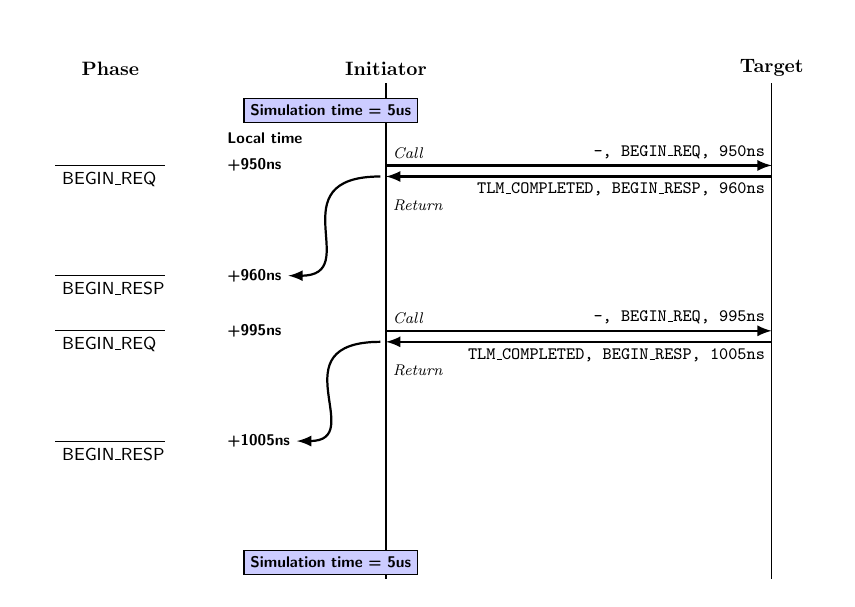
\begin{tikzpicture}[transform shape, scale=0.7]
		\clip (0.5,0) rectangle (15,10);
%		\draw[help lines] (0,0) grid (15,10);
		\path (2,9) coordinate (phase);
		\path (1,7.5) coordinate (req0);
		\path (3,7.5) coordinate (req1);
		\path (1,5.5) coordinate (rsp0);
		\path (3,5.5) coordinate (rsp1);
		\path (1,4.5) coordinate (req1_0);
		\path (3,4.5) coordinate (req1_1);
		\path (1,2.5) coordinate (rsp1_0);
		\path (3,2.5) coordinate (rsp1_1);
		\path (4,8) node(local_time) [right] {\footnotesize \textsf{\textbf{Local time}}};
		\path (4,7.5) node(10ns) [right] {\footnotesize \textsf{\textbf{+950ns}}};
		\path (4,5.5) node(20ns) [right] {\footnotesize \textsf{\textbf{+960ns}}};
		\path (4,4.5) node(35ns) [right] {\footnotesize \textsf{\textbf{+995ns}}};
		\path (4,2.5) node(45ns) [right] {\footnotesize \textsf{\textbf{+1005ns}}};
%		\path (4,1) node(wait) [right] {\footnotesize \textsf{\textbf{wait(1us)}}};
		\path (7,0) coordinate (llb);
		\path (7,9) coordinate (llt);
		\path (14,0) coordinate (rlb);
		\path (14,9) coordinate (rlt);
		\path (7,7.5) coordinate (call_left);
		\path (14,7.5) coordinate (call_right);
		\path (7,7.3) coordinate (ret_left);
		\path (14,7.3) coordinate (ret_right);
		\path (7,4.5) coordinate (call2_left);
		\path (14,4.5) coordinate (call2_right);
		\path (7,4.3) coordinate (ret2_left);
		\path (14,4.3) coordinate (ret2_right);

		\draw (phase) node[above] {\textbf{Phase}};
		\draw (llb) -- (llt)
			node[above] {\textbf{Initiator}};
		\draw (rlb) -- (rlt)
			node[above] {\textbf{Target}};
		\draw (req0) node[below right] {\small \textsf{BEGIN\_REQ}} -- (req1);
		\draw (rsp0) node[below right] {\small \textsf{BEGIN\_RESP}} -- (rsp1);
		\draw (req1_0) node[below right] {\small \textsf{BEGIN\_REQ}} -- (req1_1);
		\draw (rsp1_0) node[below right] {\small \textsf{BEGIN\_RESP}} -- (rsp1_1);
		\draw[thick,-latex] (call_left) -- (call_right);
		\draw (call_left) node[above right] {\footnotesize \emph{Call}};
		\draw (call_right) node[above left] {\small \texttt{\textbf{-, BEGIN\_REQ, 950ns}}};
		\draw[thick,latex-] (ret_left) -- (ret_right);
		\draw (ret_left) +(0,-0.3) node[below right] {\footnotesize \emph{Return}};
		\draw (ret_right) node[below left] {\small \texttt{\textbf{TLM\_COMPLETED, BEGIN\_RESP, 960ns}}};
		\draw[thick,-latex] (call2_left) -- (call2_right);
		\draw (call2_left) node[above right] {\footnotesize \emph{Call}};
		\draw (call2_right) node[above left] {\small \texttt{\textbf{-, BEGIN\_REQ, 995ns}}};
		\draw[thick,latex-] (ret2_left) -- (ret2_right);
		\draw (ret2_left) +(0,-0.3) node[below right] {\footnotesize \emph{Return}};
		\draw (ret2_right) node[below left] {\small \texttt{\textbf{TLM\_COMPLETED, BEGIN\_RESP, 1005ns}}};
		\path (6,8.5) node(100ns) [rectangle,draw,fill=blue!20] {\footnotesize \textsf{\textbf{Simulation time = 5us}}};
		\path (6,0.3) node(110ns) [rectangle,draw,fill=blue!20] {\footnotesize \textsf{\textbf{Simulation time = 5us}}};
		\path (ret_left) +(-2,0) coordinate (control_ret_left);
		\path (20ns) +(2,0) coordinate (control_20ns);
		\draw[thick,-latex] (ret_left) +(-0.1,0) .. controls (control_ret_left) and (control_20ns) .. (20ns)[above];
		\path (ret2_left) +(-2,0) coordinate (control_ret2_left);
		\path (45ns) +(2,0) coordinate (control_45ns);
		\draw[thick,-latex] (ret2_left) +(-0.1,0) .. controls (control_ret2_left) and (control_45ns) .. (45ns)[above];
	\end{tikzpicture}
\end{frame}

\begin{frame}
	\frametitle{Temporal decoupling and Quantum Keeper}
	\begin{block}{Temporal decoupling}
		Technique to enhance simulation speed specially adapted for the loosely-timed coding style.\newline
		It allows TLM models to run ahead of the current simulation time without yielding control to the simulation engine (i.e., without calling \texttt{wait(\ldots)}.
	\end{block}
	\alert{Beware of process inanition.}
	\begin{itemize}
		\item<2-> Solution:
		\begin{itemize}
			\item<2-> The Quantum Keeper
		\end{itemize}
	\end{itemize}
\end{frame}

\begin{frame}
	\frametitle{The Quantum Keeper (\texttt{tlm\_quantum\_keeper})}
	\begin{itemize}
		\item Convenience class to control avoid inanition.
	\end{itemize}
	\lstinputlisting{tlm/quantum_keeper.hh}
\end{frame}

\begin{frame}
	\frametitle{Quantum Keeper example}
	\lstinputlisting[linerange={1-13, 34-35}]{tlm/quantum_keeper_example.hh}
\end{frame}

\begin{frame}
	\frametitle{Quantum Keeper example (cont.)}
	\lstinputlisting[linerange={1-2, 14-35}]{tlm/quantum_keeper_example.hh}
\end{frame}
}

\mode<article>{
\emph{Temporal decoupling} is a powerful technique to enhance SystemC simulation speed specially adapted for the loosely-timed coding style.
Basically it consist on doing as much work as possible inside a module process without yielding the control to the SystemC simulation engine\footnote{That is, without performing any call to \texttt{wait(\ldots)}.}.
So this technique allows TLM models to run ahead of the current simulation time (as it is returned by \texttt{sc\_time\_stamp()}).

\begin{figure}[h]
	\begin{center}
	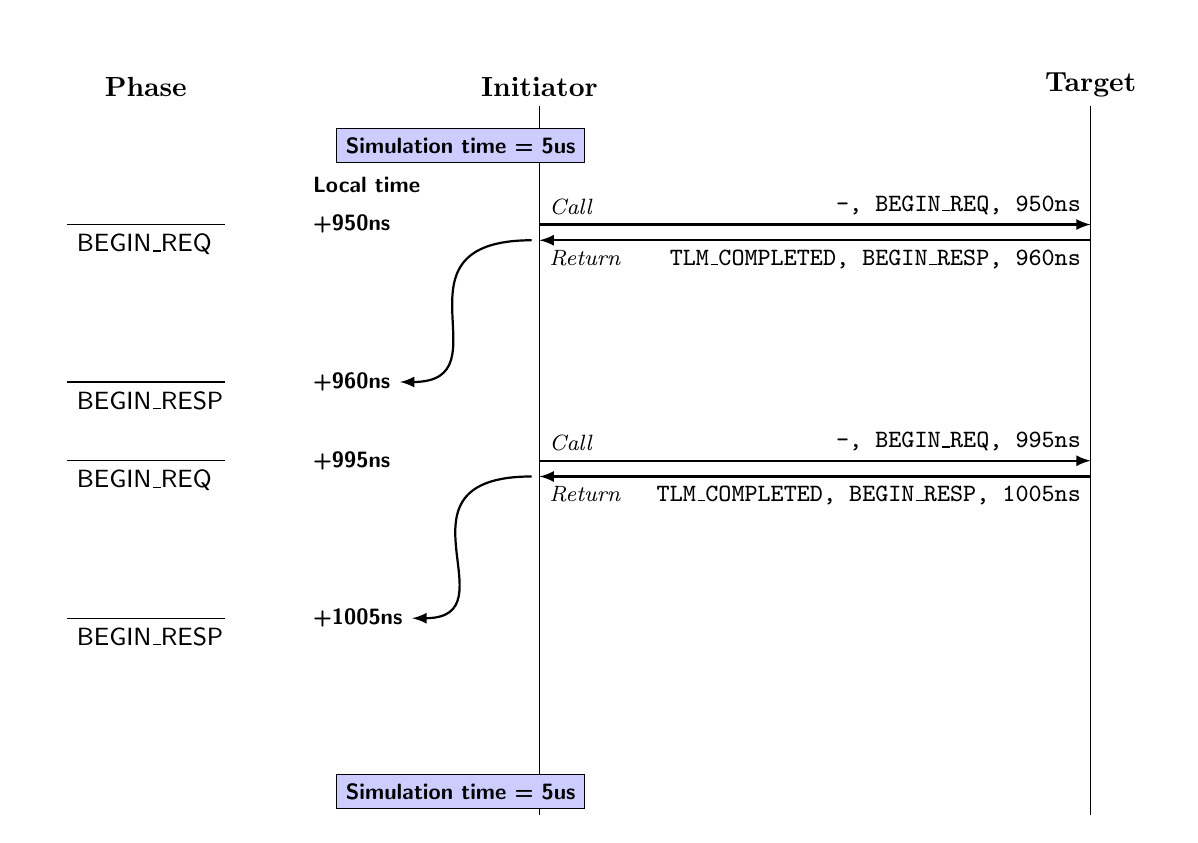
\begin{tikzpicture}
		\clip (0.5,0) rectangle (15,10);
%		\draw[help lines] (0,0) grid (15,10);
		\path (2,9) coordinate (phase);
		\path (1,7.5) coordinate (req0);
		\path (3,7.5) coordinate (req1);
		\path (1,5.5) coordinate (rsp0);
		\path (3,5.5) coordinate (rsp1);
		\path (1,4.5) coordinate (req1_0);
		\path (3,4.5) coordinate (req1_1);
		\path (1,2.5) coordinate (rsp1_0);
		\path (3,2.5) coordinate (rsp1_1);
		\path (4,8) node(local_time) [right] {\footnotesize \textsf{\textbf{Local time}}};
		\path (4,7.5) node(10ns) [right] {\footnotesize \textsf{\textbf{+950ns}}};
		\path (4,5.5) node(20ns) [right] {\footnotesize \textsf{\textbf{+960ns}}};
		\path (4,4.5) node(35ns) [right] {\footnotesize \textsf{\textbf{+995ns}}};
		\path (4,2.5) node(45ns) [right] {\footnotesize \textsf{\textbf{+1005ns}}};
%		\path (4,1) node(wait) [right] {\footnotesize \textsf{\textbf{wait(1us)}}};
		\path (7,0) coordinate (llb);
		\path (7,9) coordinate (llt);
		\path (14,0) coordinate (rlb);
		\path (14,9) coordinate (rlt);
		\path (7,7.5) coordinate (call_left);
		\path (14,7.5) coordinate (call_right);
		\path (7,7.3) coordinate (ret_left);
		\path (14,7.3) coordinate (ret_right);
		\path (7,4.5) coordinate (call2_left);
		\path (14,4.5) coordinate (call2_right);
		\path (7,4.3) coordinate (ret2_left);
		\path (14,4.3) coordinate (ret2_right);

		\draw (phase) node[above] {\textbf{Phase}};
		\draw (llb) -- (llt)
			node[above] {\textbf{Initiator}};
		\draw (rlb) -- (rlt)
			node[above] {\textbf{Target}};
		\draw (req0) node[below right] {\small \textsf{BEGIN\_REQ}} -- (req1);
		\draw (rsp0) node[below right] {\small \textsf{BEGIN\_RESP}} -- (rsp1);
		\draw (req1_0) node[below right] {\small \textsf{BEGIN\_REQ}} -- (req1_1);
		\draw (rsp1_0) node[below right] {\small \textsf{BEGIN\_RESP}} -- (rsp1_1);
		\draw[thick,-latex] (call_left) -- (call_right);
		\draw (call_left) node[above right] {\footnotesize \emph{Call}};
		\draw (call_right) node[above left] {\small \texttt{\textbf{-, BEGIN\_REQ, 950ns}}};
		\draw[thick,latex-] (ret_left) -- (ret_right);
		\draw (ret_left) node[below right] {\footnotesize \emph{Return}};
		\draw (ret_right) node[below left] {\small \texttt{\textbf{TLM\_COMPLETED, BEGIN\_RESP, 960ns}}};
		\draw[thick,-latex] (call2_left) -- (call2_right);
		\draw (call2_left) node[above right] {\footnotesize \emph{Call}};
		\draw (call2_right) node[above left] {\small \texttt{\textbf{-, BEGIN\_REQ, 995ns}}};
		\draw[thick,latex-] (ret2_left) -- (ret2_right);
		\draw (ret2_left) node[below right] {\footnotesize \emph{Return}};
		\draw (ret2_right) node[below left] {\small \texttt{\textbf{TLM\_COMPLETED, BEGIN\_RESP, 1005ns}}};
		\path (6,8.5) node(100ns) [rectangle,draw,fill=blue!20] {\footnotesize \textsf{\textbf{Simulation time = 5us}}};
		\path (6,0.3) node(110ns) [rectangle,draw,fill=blue!20] {\footnotesize \textsf{\textbf{Simulation time = 5us}}};
		\path (ret_left) +(-2,0) coordinate (control_ret_left);
		\path (20ns) +(2,0) coordinate (control_20ns);
		\draw[thick,-latex] (ret_left) +(-0.1,0) .. controls (control_ret_left) and (control_20ns) .. (20ns)[above];
		\path (ret2_left) +(-2,0) coordinate (control_ret2_left);
		\path (45ns) +(2,0) coordinate (control_45ns);
		\draw[thick,-latex] (ret2_left) +(-0.1,0) .. controls (control_ret2_left) and (control_45ns) .. (45ns)[above];
	\end{tikzpicture}
	\end{center}
	\caption{Loosely-timed coding style with temporal decoupling example.}
	\label{fig:temporal_decoupling_example}
\end{figure}

Figure~\ref{fig:temporal_decoupling_example} shows an example of a loosely-timed coding style model using temporal decoupling.
However, this technique can be dangerous, producing inanition of other processes which are waiting for SystemC to execute them.
Simply imagine that the initiator in Figure~\ref{fig:temporal_decoupling_example} never performs a \texttt{wait(\ldots)} and other initiator processes in the system never get execution.
So, when using the temporal decoupling technique care must be taken to avoid inanition.

\begin{figure}[h]
	\lstinputlisting{tlm/quantum_keeper.hh}
	\caption{The quantum keeper class definition.}
	\label{fig:quantum_keeper_definition}
\end{figure}

To facilitate the task of avoiding inanition, TLM 2.0 provides the convenience class \texttt{tlm\_quantum\_keeper} (aka. The Quantum Keeper).
It provides a set of methods for managing and interacting with the time quantum. 
It is recommended to use it in order to maintain a consistent coding style (but not compulsory).
Figure~\ref{fig:quantum_keeper_definition} shows the class definition of the quantum keeper.

\begin{figure}[h]
	\lstinputlisting{tlm/quantum_keeper_example.hh}
	\caption{Example of a loosely-timed initiator using the quantum keeper.}
	\label{fig:quantum_keeper_example}
\end{figure}

Basically this class keeps track of the module local time and synchronizes when necessary with the SystemC simulation time when necessary.
The user must define the time threshold the modules can run ahead of time using the static method \texttt{set\_global\_quantum}.
When the module local time difference with the simulation time reaches the user defined threshold the quantum keeper notifies the module that it must synchronize, that is, that is must perform a \texttt{wait(\ldots)} with the amount of time signaled by the quantum keeper.
Figure~\ref{fig:quantum_keeper_example} shows the example of a loosely-timed initiator using the quantum keeper.

Note that the user must define the time threshold for the quantum keeper globally, so no module should ever call the \texttt{set\_global\_quantum}.
Usually the quantum keeper time threshold is set up globally before or after the assembly of the simulator modules and before calling \texttt{sc\_start}.
To have a global quantum keeper time threshold helps to avoid inanition, because all the modules will share the same threshold.
The threshold is also a toggle between simulation speed and simulation accuracy, the bigger its value the less modules will yield and the faster the simulation will be. 
The smaller its value the more modules will yield and the slower the simulation will be.
}


\mode<article> {
	\clearpage
}

\section{The Generic Payload}

\mode<presentation>{

\begin{frame}
	\frametitle{The generic payload}
	\begin{block}{Objective}
		Improve interoperability between modules providing a single message type for most TLM designs.
	\end{block}
	\begin{itemize}
		\item \texttt{tlm\_generic\_payload} provides a generic message type.
		\item It is specifically aimed at memory mapped buses.
		\item It provides an extension mechanism to add ignorable extension.
		\item It can be used to generate new payload types.
	\end{itemize}
\end{frame}

\begin{frame}
	\frametitle{\texttt{tlm\_generic\_payload} class definition}
	\lstinputlisting[linerange={1-31}]{tlm/tlm_generic_payload.hh}
\end{frame}

\begin{frame}
	\frametitle{\small \texttt{tlm\_generic\_payload} class definition (contd.)}
	\lstinputlisting[linerange={31-53}]{tlm/tlm_generic_payload.hh}
\end{frame}
}

\mode<article>{
Unlike TLM 1.0, TLM 2.0 introduced a generic message type (payload).
With a generic payload, the SystemC TLM working group expects to improve the interoperability of modules written with SystemC TLM.
Effectively, one of the drawbacks of TLM 1.0 was that the payload was not standardized.
This made difficult the connection of modules that should have been easy to connect.
For example a simple address type could make two modules speaking the same protocol not interoperable.

The generic payload is specifically aimed at memory-mapped buses. 
This guarantees the interoperability of abstract models using memory-mapped buses for which precise details are unimportant.
Additionally it provides an extension mechanism which allow the designer to add details which may be \emph{ignorable}, thus not breaking the interoperability of the models, but enhancing their functionality if the connected models implement such ignorable details.

The same extension mechanism allows the designer to add bus specific details which maybe compulsory.
If such is the case, the connected models using the specific bus will need to implement such extension.
It is the responsibility of the provider of the extension to provide models which use it, models which bridge with the generic payload, or to provide coding guidelines for the usage of such extension.

The use of ignorable extensions allow the connection of two models with different payloads:
\begin{itemize}
	\item One of the models could use the generic payload without extensions and the other the generic payload with ignorable extensions.
	\item The two models could use different ignorable extensions over the generic payload.
\end{itemize}
Any of those combinations would compile, and produce an executable simulator.

However, the TLM working group recommends a disciplined use of the ignorable extensions.
Effectively, the designers could use the ignorable extensions to allow full compilation interoperability, but those models would check the non ignorable extensions at run-time, what would degrade the simulation performance or simply create simulators that would dump an error message systematically.
For that reason, there are three, \emph{an only three}\footnote{The TLM working group heavily insist on that point.} recommended alternatives for the transaction template argument of blocking and non-blocking interfaces (ordered from more interoperability to less interoperability solutions):
\begin{enumerate}
	\item \emph{Use the generic payload, with ignorable extensions.}\newline
	In this case the ignorable extensions should be clearly ignorable, that is, the models should not create an error message or fail if the extension is not available.
	Neither the model should work in degraded mode.
	Examples of correct ignorable extensions are:
	\begin{itemize}
		\item There is a clear default value for the ignorable extension.
		\item The extension contains simulation-related information, but not model behavior related information.
	\end{itemize}
	\item \emph{Define a new protocol types class containing a \texttt{typedef} for \texttt{tlm\_generic\_payload}.}\newline
	When the extensions are clearly not ignorable, but the new protocol is a clear extension of the \texttt{tlm\_generic\_payload}, this solution is recommended.
	This allows a rapid development of the new payload type thanks to the reuse the generic payload, but at the same time this ensures that compile time interoperability checking of two interconnected models.
	\item \emph{Define a new protocol types class and a new transaction type.}\newline
	When the generic payload is clearly ill adapted to create the transaction and protocol a new protocol types class and a new transaction type should be defined.
	Again, this ensures the compile time interoperability checking of two connected models.
\end{enumerate}

%\begin{figure}[h]
%	\lstinputlisting{tlm/tlm_generic_payload_types.hh}
%	\caption{The types used by the generic payload class definitions.}
%	\label{fig:tlm_generic_payload_types}
%\end{figure}

\begin{figure}[h]
	\lstinputlisting{tlm/tlm_generic_payload.hh}
	\caption{The generic payload class definition.}
	\label{fig:tlm_generic_payload_definition}
\end{figure}

Figure~\ref{fig:tlm_generic_payload_definition} shows the definition of the \texttt{tlm\_generic\_payload} class.
The initiator of a transaction is responsible of the creation of all the storage that the generic payload may require during its lifetime. 
Additionally, it is responsible of keeping the generic payload available during the lifetime of the transaction.

\begin{table}[h]
	\begin{center}
	\begin{tabular}{|l|l|l|l|}
	\hline
	\textbf{Attribute} & \textbf{Default value} & \textbf{Modifiable by} & \textbf{Modifiable by} \\
	& & \textbf{interconnect?} & \textbf{target?} \\
	\hline
	Command & \texttt{TLM\_IGNORE\_COMMAND} & No & No \\
	\hline
	Address & 0 & Yes & No \\
	\hline
	Data pointer & 0 & No & No \\
	\hline
	Data array & - & No & Yes (read) \\
	\hline
	Data length & 1 & No & No \\
	\hline
	Byte enable pointer & 0 & No & No \\
	\hline
	Byte enable array & - & No & No \\
	\hline
	Byte enable length & 1 & No & No \\
	\hline
	Streaming width & 0 & No & No \\
	\hline
	DMI allowed & false & Yes & Yes \\
	\hline
	Response status & \texttt{TLM\_INCOMPLETE\_RESPONSE} & No & Yes \\
	\hline
	Extension pointers & 0 & Yes & Yes \\
	\hline
	\end{tabular}
	\end{center}
	\caption{Generic payload default values and modifiability of attributes}
	\label{table:tlm_generic_payload_default_values}
\end{table}

When created the values of the different generic payload attributes shall be set as defined in Table~\ref{table:tlm_generic_payload_default_values}.
The copy constructor should make a shallow copy of the payload contents, that is the different pointer should be copied but not their contents.
The same applies for the assignment operator.
The \texttt{deep\_copy} method on the other side should additionally copy the contents of the pointers. Implementations of the virtual destructor should not delete the data array, the byte enable array, or any extension objects.

The generic payload attributes are not publicly accessible and should be set and get using the provided setters and getters. 
Table~\ref{table:tlm_generic_payload_default_values} shows which attributes can be modified by interconnect and target modules.
}

\subsection{The command attribute}

\mode<presentation>{

\begin{frame}
	\frametitle{The command attribute}
	\begin{itemize}
		\small
		\item<1-> Only three commands are defined:
		\lstinputlisting{tlm/tlm_command.hh}
		\item<2-> Getter and setter:
		\begin{itemize}
			\item<2-> \texttt{tlm\_command get\_command()}
			\item<2-> \texttt{void set\_command(const tlm\_command)}
		\end{itemize}
		\item<2-> Facility methods are provided to set a read/write request, and to check: \texttt{is\_read()}, \texttt{set\_read()}, \texttt{is\_write()} and \texttt{set\_write()}.
		\item<3-> Default error when command not supported: \texttt{TLM\_COMMAND\_ERROR\_RESPONSE}
		\item<4-> When the command is \texttt{TLM\_IGNORE\_COMMAND}, the target must ignore data pointer, but can use any other attributes, including extensions.
	\end{itemize}
\end{frame}

}

\mode<article>{
\begin{figure}[h]
	\lstinputlisting{tlm/tlm_command.hh}
	\caption{Definition of the different generic payload commands.}
	\label{fig:tlm_command}
\end{figure}

Figure~\ref{fig:tlm_command} shows the different commands provided by the command attribute.
Only read, write and ignore commands are provided.
The generic payload provides a setter and getter to set and get the command, and convenience methods to set and get them: \texttt{is\_read()}, \texttt{is\_write()}, \texttt{set\_read()}, \texttt{set\_write()}.

When receiving a read command the target should fill the array pointed by the data pointer attribute.
When receiving a write command the target should copy the array pointed by the data pointer attribute.
If the target is unable to execute a read or write command, it shall generate a standard error response (\texttt{TLM\_COMMAND\_ERROR\_RESPONSE} is recommended).
When receiving an ignore command the target should ignore the contents of the data pointer, but can use any other attribute in the payload, including extensions.
}

\subsection{The address attribute}

\mode<presentation>{

\begin{frame}
	\frametitle{The address attribute}
	\begin{itemize}
		\item<1-> It corresponds to the first byte in the array pointed by the data pointer attribute.
		\item<1-> Getter and setter:
		\begin{itemize}
			\item<1-> \texttt{sc\_dt::uint64 get\_address()}
			\item<1-> \texttt{void set\_address(const sc\_dt::uint64)}
		\end{itemize}
		\item<2-> Formula: \textbf{$address\_attribute + (array\_index \% streaming\_width)$}
		\item<3-> Default error when error in address: \texttt{TLM\_ADDRESS\_ERROR\_RESPONSE}
		\item<3-> Interconnect modules may change its value (for example when a translation needs to be made).
	\end{itemize}
\end{frame}
}

\mode<article>{
The address received by the target should be considered as the first byte to be read from or written to the local array in the target.
It always corresponds to the first byte in the array pointed by the data pointer attribute.

A byte at a given index in the data array shall be transferred to or from the address given by the formula \textbf{$address\_attribute + (array\_index \% streaming\_width)$}.

If the requested command can not be performed in the given address (or address range) an standard error should be returned (\texttt{TLM\_ADDRESS\_ERROR\_RESPONSE} is recommended).

The address attribute is set by the initiator module. Target module should not modify it, however, interconnect modules can modify its value.
It could be the case if the interconnect module needs to do some kind of address translation on the transaction.
}

\subsection{The data pointer attribute}

\mode<presentation>{

\begin{frame}
	\frametitle{The data pointer attribute}
	\begin{itemize}
		\item<1-> Buffer allocated by the initiator module to perform the read/write command.
		\item<1-> Getter and setter:
		\begin{itemize}
			\item<1-> \texttt{unsigned char* get\_data\_ptr()}
			\item<1-> \texttt{void set\_data\_ptr(unsigned char *)}
		\end{itemize}
		\item<2-> Must be always different than 0 (\texttt{NULL}).
		\item<2-> Should never be modified by interconnect modules.
		\item<2-> The size of the buffer must be bigger than the number of bytes to read/write (the data lengt attribute).
	\end{itemize}
\end{frame}

}

\mode<article>{
The data pointer attribute should point to a buffer allocated by the initiator module.
The data pointer should always be set to something different than 0 before calling the transport interface.
Such buffer should contain the data to be written into the target on write command, and a buffer to write the data to be read from the target on read command.
Interconnect modules should never modify the contents of the buffer.
The size of the buffer should always be bigger than the number of bytes to read/write (the data length attribute).
}

\subsection{The data length attribute}

\mode<presentation>{

\begin{frame}
	\frametitle{The data length attribute}
	\begin{itemize}
		\item<1-> It represents the length in bytes to be read/written, inclusive for any bytes disabled by the byte enable attribute.
		\item<1-> Getter and setter:
		\begin{itemize}
			\item<1-> \texttt{unsigned int get\_data\_length()}
			\item<1-> \texttt{void set\_data\_length(const unsigned int)}
		\end{itemize}
		\item<2-> If it is bigger than the template parameter BUSWIDTH, the transfer is considered as a burst transfer.
		\item<2-> Default error when error due to the data length attribute: \texttt{TLM\_BURST\_ERROR\_RESPONSE}.
	\end{itemize}
\end{frame}

}

\mode<article>{
It represents the length in bytes to be read/written, inclusive for any bytes disabled by the byte enable attribute.
This attribute shall be set by the initiator module, and not modified by any interconnect or target module.

If the data length is bigger than the template parameter \texttt{BUSWIDTH} (in bits) the transfer is considered as a burst transfer.
The size of the transfer on those cases is the \texttt{BUSWIDTH}.
If the data length is smaller than or equal to \texttt{BUSWIDTH} the transfer is a word transfer, not a burst transfer.

If the target can not satisfy the request given the received data length, it should generate a standard error response (\texttt{TLM\_BURST\_ERROR\_RESPONSE} is recommended).
}

\subsection{The byte enable pointer and the byte enable length attributes}

\mode<presentation>{

\begin{frame}
	\frametitle{The byte enable pointer and length attributes}
	\begin{itemize}
		\item<1-> Define the bytes that should be read from or written to the data buffer.
		\item<1-> The byte enable length defines the size of the byte enable array.
		\item<1-> Getter and setter:
		\begin{itemize}
			\item<1-> \texttt{unsigned char* get\_byte\_enable\_ptr()}
			\item<1-> \texttt{void set\_byte\_enable\_ptr(unsigned char *)}
			\item<1-> \texttt{unsigned int get\_byte\_enable\_length()}
			\item<1-> \texttt{void set\_byte\_enable\_length(const unsigned int)}
		\end{itemize}
		\item<2-> Formula: $byte\_enable\_array\_index = data\_array\_index \% byte\_enable\_length$
		\item<2-> If length is equal to 0, the byte enable array can be ignored.
		\item<3-> Default error response because byte enable error: \texttt{TLM\_BYTE\_ENABLE\_ERROR\_RESPONSE}
	\end{itemize}
\end{frame}
}

\mode<article>{
Those couple of attributes define the bytes that should be read from or written to the data buffer.
The byte enable length attribute defines the size of the byte enable pointer.
The byte enable pointer attribute points to an array of booleans that defines the mask of bytes that should be considered(true value)/ignored(false value).

If the byte enable length attribute is smaller than the data length attribute, the contents of the byte enable pointer should be considered as many times as necessary to match the data length attribute.
The following formula can be used $byte\_enable\_array\_index = data\_array\_index \% byte\_enable\_length$.

If the byte enabled pointer is equal to 0 the byte enable length attribute must be ignored, and bytes enables should be also ignored (all the contents of the data array should be considered).

If the target can not process the requested transaction because of the byte enable pointer or the byte enable length attributes, a standard error should be returned (TLM\_BYTE\_ENABLE\_ERROR\_RESPONSE is recommended).
}

\subsection{The streaming width attribute}

\mode<presentation>{

\begin{frame}
	\frametitle{The streaming width attribute}
	\begin{itemize}
		\item<1-> It determines the width of the stream, that is, the number of bytes transferred on each beat.
		\item<1-> Getter and setter:
		\begin{itemize}
			\item<1-> \texttt{unsigned int get\_streaming\_width()}
			\item<1-> \texttt{void set\_streaming\_width(unsigned int)}
		\end{itemize}
		\item<2-> Formula: \textbf{$address\_attribute + (array\_index \% streaming\_width)$}
		\item<2-> If its value is equal to 0, then the transfer is considered as a normal transfer (or burst transfer).
		\item<3-> Default error on stream width error: \texttt{TLM\_BURST\_ERROR\_RESPONSE}.
	\end{itemize}
\end{frame}

}

\mode<article>{
Streaming affects the way a component should interpret the data array. 
A stream consists of a sequence of data transfers occurring on successive notional beats. 
The streaming width attribute shall determine the width of the stream, that is, the number of bytes transferred on each beat.

The address to or from which each byte is being copied in the target shall be reset to the value of the address attribute at the start of each beat.

With respect to the interpretation of the data array, a transaction with a non-zero streaming width shall be functionally equivalent to a sequence of transactions each having the same address as the original transaction, each having a data length attribute equal to the streaming width of the original, and each with a data array that effectively steps down the original data array maintaining the sequence of bytes.

A streaming width of 0 shall be interpreted in the same way as a streaming width greater than or equal to the value of the data length attribute, that is, the data transfer is a normal transfer, not a streaming transfer.

If the target module can not process the transfer because of the streaming width attribute a standard error should be returned (\texttt{TLM\_BURST\_ERROR\_RESPONSE} is recommended).
}

\subsection{Endianess}

\mode<presentation>{

\begin{frame}
	\frametitle{Endianess}
	\begin{block}{}
		In order to interpret the contents of the data pointer array TLM 2.0 defines that the data transferred should be sent using the host endianness.
	\end{block}
\end{frame}

}

\mode<article>{
In order to interpret the contents of the data pointer array TLM 2.0 defines that the data transferred should be sent using the host endianness.
}

\subsection{DMI allowed attribute}

\mode<presentation>{

\begin{frame}
	\frametitle{DMI allowed attribute}
	\begin{itemize}
		\item<1-> Thanks to this attribute the target module can give a hint to the initiator module signaling if the target supports or not DMI for the current request.
		\item<1-> Getter and setter:
		\begin{itemize}
			\item<1-> \texttt{void set\_dmi\_allowed(bool)}
			\item<1-> \texttt{bool get\_dmi\_allowed()}
		\end{itemize}
	\end{itemize}
\end{frame}
}

\mode<article>{
Thanks to this attribute the target module can give a hint to the initiator module signaling if the target supports or not DMI for the current request.
}

\subsection{The response status attribute}

\mode<presentation>{

\begin{frame}
	\frametitle{The response status attribute}
	\begin{itemize}
		\item<1-> Possible error attribute values:
		\lstinputlisting{tlm/tlm_response_status.hh}
		\item<1-> Getter and setter:
		\begin{itemize}
			\item<1-> \texttt{tlm\_response\_status get\_response\_status()}
			\item<1-> \texttt{void set\_response\_status(const tlm\_response\_status)}
		\end{itemize}
		\item<2-> Helper methods:
		\begin{itemize}
			\item<2-> \texttt{std::string get\_response\_string()}
			\item<2-> \texttt{bool is\_response\_ok()}
			\item<2-> \texttt{bool is\_response\_error()}
		\end{itemize}
	\end{itemize}
\end{frame}
}

\mode<article>{
\begin{figure}[h]
	\lstinputlisting{tlm/tlm_response_status.hh}
	\caption{Definition of the different response status values.}
	\label{fig:tlm_response_status_definition}
\end{figure}

\begin{table}[h]
	\begin{center}
	\begin{tabular}{|l|l|}
		\hline
		\textbf{Error response} & \textbf{Interpretation} \\
		\hline
		\texttt{TLM\_ADDRESS\_ERROR\_RESPONSE} & Unable to act upon the address attribute, \\
		& or address out of range\\
		\hline
		\texttt{TLM\_COMMAND\_ERROR\_RESPONSE} & Unable to execute the command \\
		\hline
		\texttt{TLM\_BURST\_ERROR\_RESPONSE} & Unable to act upon the data length or streaming width \\
		\hline
		\texttt{TLM\_BYTE\_ENABLE\_ERROR\_RESPONSE} & Unable to act upon the byte enable \\
		\hline
		\texttt{TLM\_GENERIC\_ERROR\_RESPONSE} & Any other error	\\
		\hline
	\end{tabular}
	\end{center}
	\caption{Error response values}
	\label{table:response_status_errors}
\end{table}

Figure~\ref{fig:tlm_response_status_definition} shows the response status attribute possible values.
This attribute is used by the target module to signal the success (\texttt{TLM\_OK\_RESPONSE}) if the transaction could successfully handled, and to an error otherwise, following the Table~\ref{table:response_status_errors}.
The initiator should set this attribute to \texttt{TLM\_INCOMPLETE\_RESPONSE}, and no interconnect module should modify it, because it means that the target module has not still handled the transaction.
}

\subsection{The extension mechanism}

\mode<article>{
The extension mechanism is out of the scope of this tutorial.
For a detailed explanation refer to the Accellera TLM 2.0 User Manual.
}


\mode<article>{
	\clearpage
}

\section{Message charts examples}

\mode<presentation>{

\begin{frame}
	\frametitle{Message charts examples}
	\begin{itemize}
		\item<1-> Untimed
		\item<1-> Loosely-timed with timing annotation
		\item<1-> Loosely-timed with sync
		\item<1-> Loosely-timed with temporal decoupling
		\item<1-> Loosely-timed with temporal decoupling and synchronization-on-demand
		\item<1-> Loosely-timed with temporal decoupling and quantum
		\item<1-> Approximately-timed using backward path
		\item<1-> Approximately-timed with timing annotation
		\item<1-> Approximately-timed with polling
	\end{itemize}
\end{frame}

}

\mode<article>{
In the following subsections you will find charts explaining the message exchanges examples when using the different coding styles.
}

\subsection{Untimed}

\mode<presentation>{
\begin{frame}
	\frametitle{Untimed}

\begin{figure}[h]
	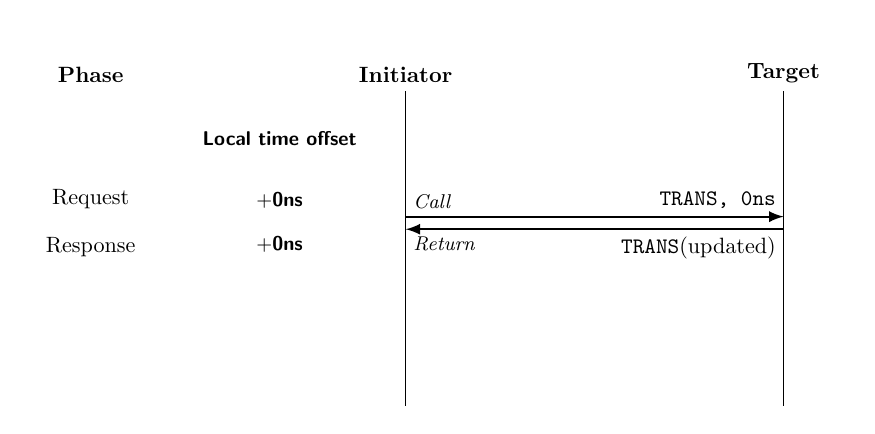
\begin{tikzpicture}[transform shape,scale=0.8]
		\clip (1,0) rectangle (14,6);
%		\draw[help lines] (0,0) grid (15,10);
		\path (2,5) coordinate (phase);
		\path (2,3) coordinate (req);
		\path (2,2.8) coordinate (rsp);
		\path (5,4) coordinate (time);
		\path (5,3) coordinate (0ns);
		\path (5,2.8) coordinate (0nstext);
		\path (7,0) coordinate (llb);
		\path (7,5) coordinate (llt);
		\path (13,0) coordinate (rlb);
		\path (13,5) coordinate (rlt);
		\path (7,3) coordinate (call_left);
		\path (13,3) coordinate (call_right);
		\path (7,2.8) coordinate (ret_left);
		\path (13,2.8) coordinate (ret_right);

		\onslide*<1-> {
		\draw (phase) node[above] {\textbf{Phase}};
		\draw (llb) -- (llt)
			node[above] {\textbf{Initiator}};
		\draw (rlb) -- (rlt)
			node[above] {\textbf{Target}};
		\draw (time) node[above] {\small \textbf{\textsf{Local time offset}}};
		}
		\onslide*<2-> {
		\draw (req) node[above] {Request};
		\draw (0ns) node[above] {\small \textbf{\textsf{$+$0ns}}};
		\draw[thick,-latex] (call_left) -- (call_right);
		\draw (call_left) node[above right] {\small \emph{Call}};
		\draw (call_right) node[above left] {\texttt{\textbf{TRANS, 0ns}}};
		}
		\onslide*<3-> {
		\draw (rsp) node[below] {Response};
		\draw[thick,latex-] (ret_left) -- (ret_right);
		\draw (ret_left) node[below right] {\small \emph{Return}};
		\draw (ret_right) node[below left] {\texttt{\textbf{TRANS}}(updated)};
		\draw (0nstext) node[below] {\small \textbf{\textsf{$+$0ns}}};
		}
	\end{tikzpicture}
\end{figure}
\end{frame}
}

\mode<article>{
Figure~\ref{fig:chart_untimed} shows the message exchange that occur when using the untimed coding style.

\begin{figure}[h]
	\begin{center}
	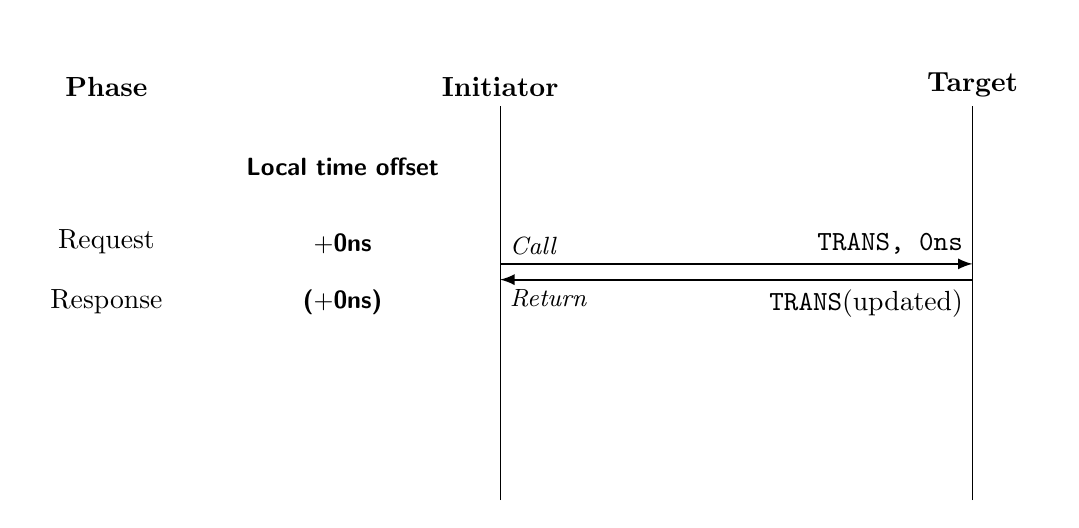
\begin{tikzpicture}
		\clip (1,0) rectangle (14,6);
%		\draw[help lines] (0,0) grid (15,10);
		\path (2,5) coordinate (phase);
		\path (2,3) coordinate (req);
		\path (2,2.8) coordinate (rsp);
		\path (5,4) coordinate (time);
		\path (5,3) coordinate (0ns);
		\path (5,2.8) coordinate (0nstext);
		\path (7,0) coordinate (llb);
		\path (7,5) coordinate (llt);
		\path (13,0) coordinate (rlb);
		\path (13,5) coordinate (rlt);
		\path (7,3) coordinate (call_left);
		\path (13,3) coordinate (call_right);
		\path (7,2.8) coordinate (ret_left);
		\path (13,2.8) coordinate (ret_right);

		\draw (phase) node[above] {\textbf{Phase}};
		\draw (llb) -- (llt)
			node[above] {\textbf{Initiator}};
		\draw (rlb) -- (rlt)
			node[above] {\textbf{Target}};
		\draw (req) node[above] {Request};
		\draw (rsp) node[below] {Response};
		\draw (time) node[above] {\small \textbf{\textsf{Local time offset}}};
		\draw (0ns) node[above] {\small \textbf{\textsf{$+$0ns}}};
		\draw (0nstext) node[below] {\small \textbf{\textsf{($+$0ns)}}};
		\draw[thick,-latex] (call_left) -- (call_right);
		\draw (call_left) node[above right] {\small \emph{Call}};
		\draw (call_right) node[above left] {\texttt{\textbf{TRANS, 0ns}}};
		\draw[thick,latex-] (ret_left) -- (ret_right);
		\draw (ret_left) node[below right] {\small \emph{Return}};
		\draw (ret_right) node[below left] {\texttt{\textbf{TRANS}}(updated)};
	\end{tikzpicture}
	\end{center}
	\caption{Untimed coding style message chart.}
	\label{fig:chart_untimed}
\end{figure}
}

\subsection{Loosely-timed with timing annotation}

\mode<presentation>{

\begin{frame}
	\frametitle{Loosely-timed with timing annotation}

\begin{figure}[h]
	\begin{center}
	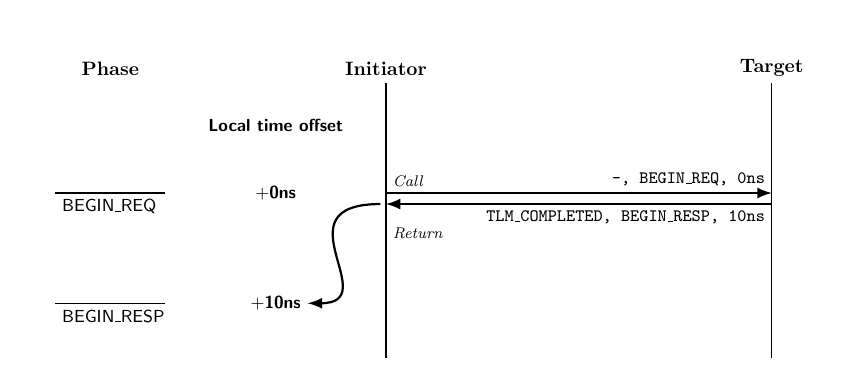
\begin{tikzpicture}[transform shape,scale=0.7]
		\clip (0.5,0) rectangle (15,6);
%		\draw[help lines] (0,0) grid (15,10);
		\path (2,5) coordinate (phase);
		\path (1,3) coordinate (req0);
		\path (3,3) coordinate (req1);
		\path (1,1) coordinate (rsp0);
		\path (3,1) coordinate (rsp1);
		\path (5,4) coordinate (time);
		\path (5,3) coordinate (0ns);
		\path (5,1) coordinate (10ns);
		\path (7,0) coordinate (llb);
		\path (7,5) coordinate (llt);
		\path (14,0) coordinate (rlb);
		\path (14,5) coordinate (rlt);
		\path (7,3) coordinate (call_left);
		\path (14,3) coordinate (call_right);
		\path (7,2.8) coordinate (ret_left);
		\path (14,2.8) coordinate (ret_right);

		\draw (phase) node[above] {\textbf{Phase}};
		\draw (llb) -- (llt)
			node[above] {\textbf{Initiator}};
		\draw (rlb) -- (rlt)
			node[above] {\textbf{Target}};
		\draw (req0) node[below right] {\small \textsf{BEGIN\_REQ}} -- (req1);
		\draw (rsp0) node[below right] {\small \textsf{BEGIN\_RESP}} -- (rsp1);
		\draw (time) node[above] {\small \textbf{\textsf{Local time offset}}};
		\draw (0ns) node {\small \textbf{\textsf{$+$0ns}}};
		\draw (10ns) node(10nstext) {\small \textbf{\textsf{$+$10ns}}};
		\draw[thick,-latex] (call_left) -- (call_right);
		\draw (call_left) node[above right] {\footnotesize \emph{Call}};
		\draw (call_right) node[above left] {\small \texttt{\textbf{-, BEGIN\_REQ, 0ns}}};
		\draw[thick,latex-] (ret_left) -- (ret_right);
		\draw (ret_left) +(0,-0.3) node[below right] {\footnotesize \emph{Return}};
		\draw (ret_right) node[below left] {\small \texttt{\textbf{TLM\_COMPLETED, BEGIN\_RESP, 10ns}}};
		\path (ret_left) +(-2,0) coordinate (control_ret_left);
		\path (10nstext)[above] +(2,0) coordinate (control_10nstext);
		\draw[thick,-latex] (ret_left) +(-0.1,0) .. controls (control_ret_left) and (control_10nstext) .. (10nstext)[above];
	\end{tikzpicture}
	\end{center}
\end{figure}

\end{frame}

}

\mode<article>{
Figure~\ref{fig:chart_lt_with_timing_annotation} shows the message exchange that occur when using the loosely-timed coding style with timing annotation.

\begin{figure}[h]
	\begin{center}
	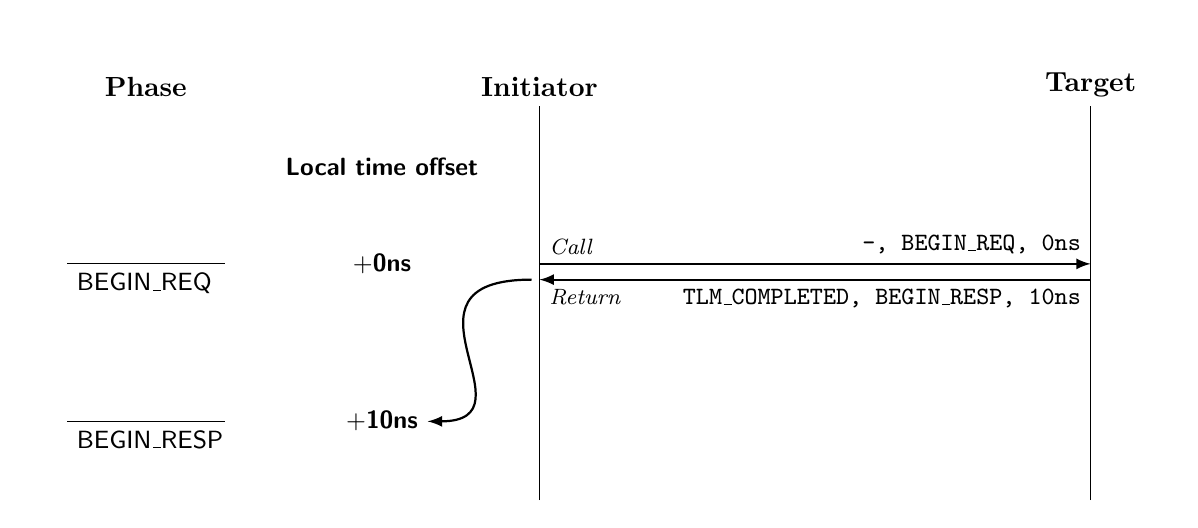
\begin{tikzpicture}
		\clip (0.5,0) rectangle (15,6);
%		\draw[help lines] (0,0) grid (15,10);
		\path (2,5) coordinate (phase);
		\path (1,3) coordinate (req0);
		\path (3,3) coordinate (req1);
		\path (1,1) coordinate (rsp0);
		\path (3,1) coordinate (rsp1);
		\path (5,4) coordinate (time);
		\path (5,3) coordinate (0ns);
		\path (5,1) coordinate (10ns);
		\path (7,0) coordinate (llb);
		\path (7,5) coordinate (llt);
		\path (14,0) coordinate (rlb);
		\path (14,5) coordinate (rlt);
		\path (7,3) coordinate (call_left);
		\path (14,3) coordinate (call_right);
		\path (7,2.8) coordinate (ret_left);
		\path (14,2.8) coordinate (ret_right);

		\draw (phase) node[above] {\textbf{Phase}};
		\draw (llb) -- (llt)
			node[above] {\textbf{Initiator}};
		\draw (rlb) -- (rlt)
			node[above] {\textbf{Target}};
		\draw (req0) node[below right] {\small \textsf{BEGIN\_REQ}} -- (req1);
		\draw (rsp0) node[below right] {\small \textsf{BEGIN\_RESP}} -- (rsp1);
		\draw (time) node[above] {\small \textbf{\textsf{Local time offset}}};
		\draw (0ns) node {\small \textbf{\textsf{$+$0ns}}};
		\draw (10ns) node(10nstext) {\small \textbf{\textsf{$+$10ns}}};
		\draw[thick,-latex] (call_left) -- (call_right);
		\draw (call_left) node[above right] {\footnotesize \emph{Call}};
		\draw (call_right) node[above left] {\small \texttt{\textbf{-, BEGIN\_REQ, 0ns}}};
		\draw[thick,latex-] (ret_left) -- (ret_right);
		\draw (ret_left) node[below right] {\footnotesize \emph{Return}};
		\draw (ret_right) node[below left] {\small \texttt{\textbf{TLM\_COMPLETED, BEGIN\_RESP, 10ns}}};
		\path (ret_left) +(-2,0) coordinate (control_ret_left);
		\path (10nstext)[above] +(2,0) coordinate (control_10nstext);
		\draw[thick,-latex] (ret_left) +(-0.1,0) .. controls (control_ret_left) and (control_10nstext) .. (10nstext)[above];
	\end{tikzpicture}
	\end{center}
	\caption{Loosely-timed coding style with timing annotation message chart.}
	\label{fig:chart_lt_with_timing_annotation}
\end{figure}
}

\clearpage
\subsection{Loosely-timed with sync}

\mode<presentation>{

\begin{frame}
	\frametitle{Loosely-timed with sync}

\begin{figure}[h]
	\begin{center}
	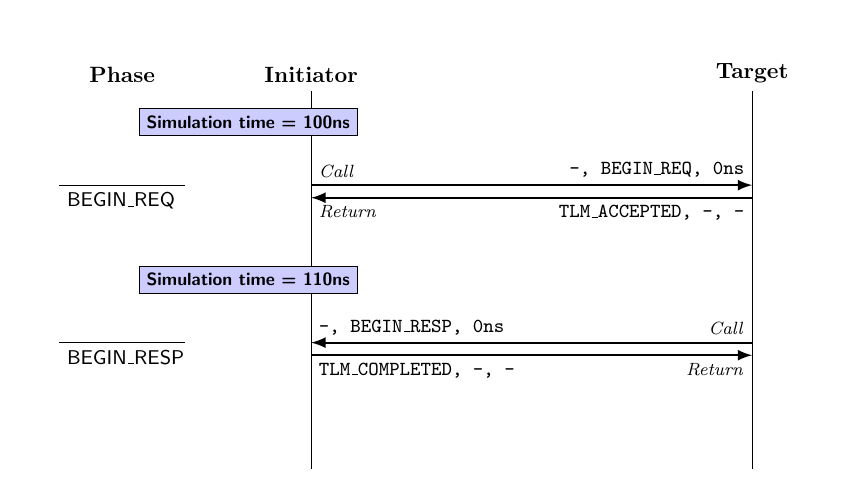
\begin{tikzpicture}[transform shape,scale=0.8]
		\clip (2.5,0) rectangle (15,7);
%		\draw[help lines] (0,0) grid (15,10);
		\path (4,6) coordinate (phase);
		\path (3,4.5) coordinate (req0);
		\path (5,4.5) coordinate (req1);
		\path (3,2) coordinate (rsp0);
		\path (5,2) coordinate (rsp1);
		\path (7,0) coordinate (llb);
		\path (7,6) coordinate (llt);
		\path (14,0) coordinate (rlb);
		\path (14,6) coordinate (rlt);
		\path (7,4.5) coordinate (call_left);
		\path (14,4.5) coordinate (call_right);
		\path (7,4.3) coordinate (ret_left);
		\path (14,4.3) coordinate (ret_right);
		\path (7,2) coordinate (call2_left);
		\path (14,2) coordinate (call2_right);
		\path (7,1.8) coordinate (ret2_left);
		\path (14,1.8) coordinate (ret2_right);

		\draw (phase) node[above] {\textbf{Phase}};
		\draw (llb) -- (llt)
			node[above] {\textbf{Initiator}};
		\draw (rlb) -- (rlt)
			node[above] {\textbf{Target}};
		\draw (req0) node[below right] {\small \textsf{BEGIN\_REQ}} -- (req1);
		\draw (rsp0) node[below right] {\small \textsf{BEGIN\_RESP}} -- (rsp1);
		\draw[thick,-latex] (call_left) -- (call_right);
		\draw (call_left) node[above right] {\footnotesize \emph{Call}};
		\draw (call_right) node[above left] {\small \texttt{\textbf{-, BEGIN\_REQ, 0ns}}};
		\draw[thick,latex-] (ret_left) -- (ret_right);
		\draw (ret_left) node[below right] {\footnotesize \emph{Return}};
		\draw (ret_right) node[below left] {\small \texttt{\textbf{TLM\_ACCEPTED, -, -}}};
		\draw[thick,latex-] (call2_left) -- (call2_right);
		\draw (call2_right) node[above left] {\footnotesize \emph{Call}};
		\draw (call2_left) node[above right] {\small \texttt{\textbf{-, BEGIN\_RESP, 0ns}}};
		\draw[thick,-latex] (ret2_left) -- (ret2_right);
		\draw (ret2_right) node[below left] {\footnotesize \emph{Return}};
		\draw (ret2_left) node[below right] {\small \texttt{\textbf{TLM\_COMPLETED, -, -}}};
		\path (6,5.5) node(100ns) [rectangle,draw,fill=blue!20] {\footnotesize \textsf{\textbf{Simulation time = 100ns}}};
		\path (6,3) node(110ns) [rectangle,draw,fill=blue!20] {\footnotesize \textsf{\textbf{Simulation time = 110ns}}};
	\end{tikzpicture}
	\end{center}
\end{figure}
\end{frame}
}

\mode<article>{
Figure~\ref{fig:chart_lt_with_sync} shows the message exchange that occur when using the loosely-timed coding style with sync.

\begin{figure}[h]
	\begin{center}
	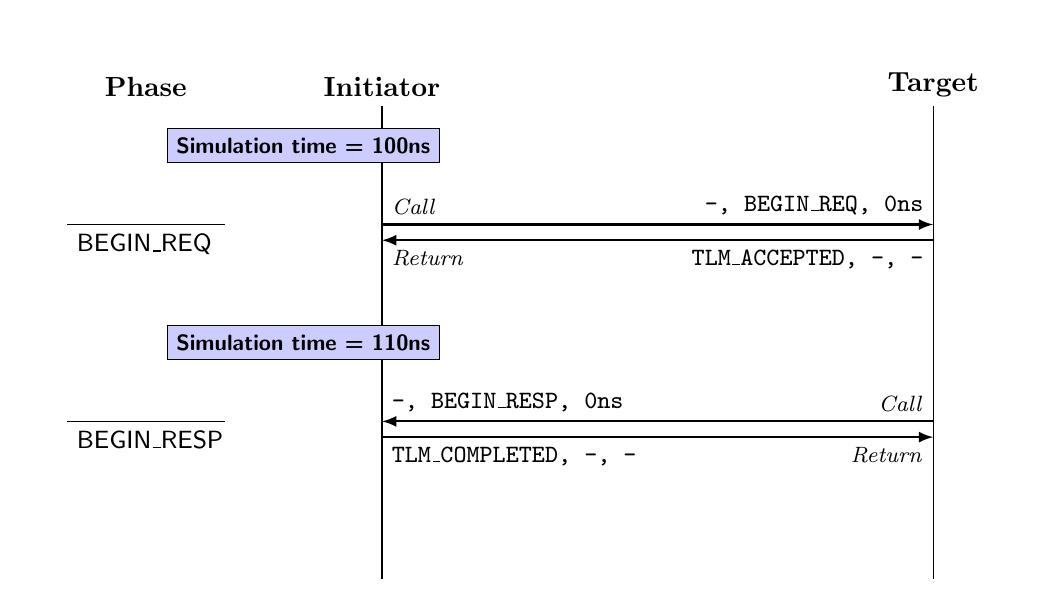
\begin{tikzpicture}
		\clip (2.5,0) rectangle (15,7);
%		\draw[help lines] (0,0) grid (15,10);
		\path (4,6) coordinate (phase);
		\path (3,4.5) coordinate (req0);
		\path (5,4.5) coordinate (req1);
		\path (3,2) coordinate (rsp0);
		\path (5,2) coordinate (rsp1);
		\path (7,0) coordinate (llb);
		\path (7,6) coordinate (llt);
		\path (14,0) coordinate (rlb);
		\path (14,6) coordinate (rlt);
		\path (7,4.5) coordinate (call_left);
		\path (14,4.5) coordinate (call_right);
		\path (7,4.3) coordinate (ret_left);
		\path (14,4.3) coordinate (ret_right);
		\path (7,2) coordinate (call2_left);
		\path (14,2) coordinate (call2_right);
		\path (7,1.8) coordinate (ret2_left);
		\path (14,1.8) coordinate (ret2_right);

		\draw (phase) node[above] {\textbf{Phase}};
		\draw (llb) -- (llt)
			node[above] {\textbf{Initiator}};
		\draw (rlb) -- (rlt)
			node[above] {\textbf{Target}};
		\draw (req0) node[below right] {\small \textsf{BEGIN\_REQ}} -- (req1);
		\draw (rsp0) node[below right] {\small \textsf{BEGIN\_RESP}} -- (rsp1);
		\draw[thick,-latex] (call_left) -- (call_right);
		\draw (call_left) node[above right] {\footnotesize \emph{Call}};
		\draw (call_right) node[above left] {\small \texttt{\textbf{-, BEGIN\_REQ, 0ns}}};
		\draw[thick,latex-] (ret_left) -- (ret_right);
		\draw (ret_left) node[below right] {\footnotesize \emph{Return}};
		\draw (ret_right) node[below left] {\small \texttt{\textbf{TLM\_ACCEPTED, -, -}}};
		\draw[thick,latex-] (call2_left) -- (call2_right);
		\draw (call2_right) node[above left] {\footnotesize \emph{Call}};
		\draw (call2_left) node[above right] {\small \texttt{\textbf{-, BEGIN\_RESP, 0ns}}};
		\draw[thick,-latex] (ret2_left) -- (ret2_right);
		\draw (ret2_right) node[below left] {\footnotesize \emph{Return}};
		\draw (ret2_left) node[below right] {\small \texttt{\textbf{TLM\_COMPLETED, -, -}}};
		\path (6,5.5) node(100ns) [rectangle,draw,fill=blue!20] {\footnotesize \textsf{\textbf{Simulation time = 100ns}}};
		\path (6,3) node(110ns) [rectangle,draw,fill=blue!20] {\footnotesize \textsf{\textbf{Simulation time = 110ns}}};
	\end{tikzpicture}
	\end{center}
	\caption{Loosely-timed coding style with sync message chart.}
	\label{fig:chart_lt_with_sync}
\end{figure}
}

\clearpage
\subsection{Loosely-timed with temporal decoupling}

\mode<presentation>{

\begin{frame}
	\frametitle{Loosely-timed with temporal decoupling}

\begin{figure}[h]
	\begin{center}
	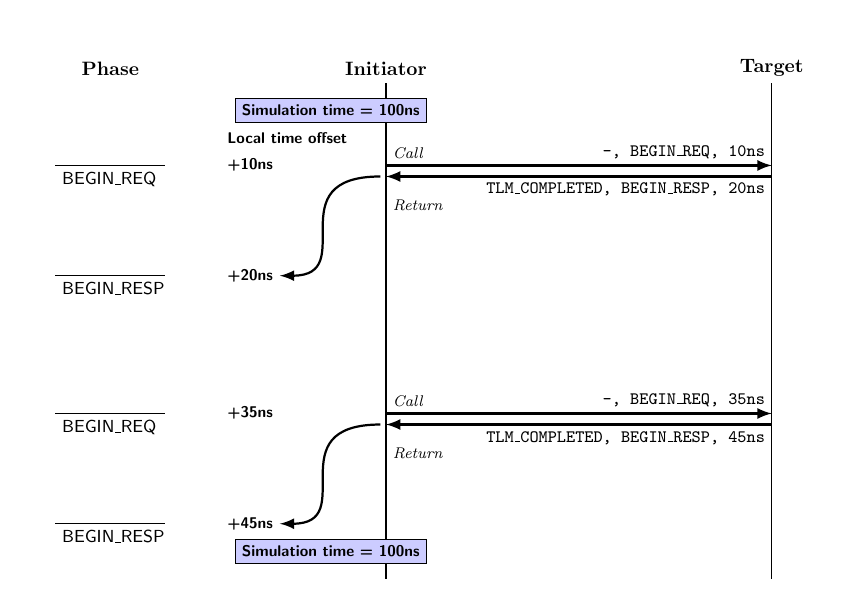
\begin{tikzpicture}[transform shape,scale=0.7]
		\clip (0.5,0) rectangle (15,10);
%		\draw[help lines] (0,0) grid (15,10);
		\path (2,9) coordinate (phase);
		\path (1,7.5) coordinate (req0);
		\path (3,7.5) coordinate (req1);
		\path (1,5.5) coordinate (rsp0);
		\path (3,5.5) coordinate (rsp1);
		\path (1,3) coordinate (req1_0);
		\path (3,3) coordinate (req1_1);
		\path (1,1) coordinate (rsp1_0);
		\path (3,1) coordinate (rsp1_1);
		\path (4,8) node(local_time) [right] {\footnotesize \textsf{\textbf{Local time offset}}};
		\path (4,7.5) node(10ns) [right] {\footnotesize \textsf{\textbf{+10ns}}};
		\path (4,5.5) node(20ns) [right] {\footnotesize \textsf{\textbf{+20ns}}};
		\path (4,3) node(35ns) [right] {\footnotesize \textsf{\textbf{+35ns}}};
		\path (4,1) node(45ns) [right] {\footnotesize \textsf{\textbf{+45ns}}};
		\path (7,0) coordinate (llb);
		\path (7,9) coordinate (llt);
		\path (14,0) coordinate (rlb);
		\path (14,9) coordinate (rlt);
		\path (7,7.5) coordinate (call_left);
		\path (14,7.5) coordinate (call_right);
		\path (7,7.3) coordinate (ret_left);
		\path (14,7.3) coordinate (ret_right);
		\path (7,3) coordinate (call2_left);
		\path (14,3) coordinate (call2_right);
		\path (7,2.8) coordinate (ret2_left);
		\path (14,2.8) coordinate (ret2_right);

		\draw (phase) node[above] {\textbf{Phase}};
		\draw (llb) -- (llt)
			node[above] {\textbf{Initiator}};
		\draw (rlb) -- (rlt)
			node[above] {\textbf{Target}};
		\draw (req0) node[below right] {\small \textsf{BEGIN\_REQ}} -- (req1);
		\draw (rsp0) node[below right] {\small \textsf{BEGIN\_RESP}} -- (rsp1);
		\draw (req1_0) node[below right] {\small \textsf{BEGIN\_REQ}} -- (req1_1);
		\draw (rsp1_0) node[below right] {\small \textsf{BEGIN\_RESP}} -- (rsp1_1);
		\draw[thick,-latex] (call_left) -- (call_right);
		\draw (call_left) node[above right] {\footnotesize \emph{Call}};
		\draw (call_right) node[above left] {\small \texttt{\textbf{-, BEGIN\_REQ, 10ns}}};
		\draw[thick,latex-] (ret_left) -- (ret_right);
		\draw (ret_left) +(0,-0.3) node[below right] {\footnotesize \emph{Return}};
		\draw (ret_right) node[below left] {\small \texttt{\textbf{TLM\_COMPLETED, BEGIN\_RESP, 20ns}}};
		\draw[thick,-latex] (call2_left) -- (call2_right);
		\draw (call2_left) node[above right] {\footnotesize \emph{Call}};
		\draw (call2_right) node[above left] {\small \texttt{\textbf{-, BEGIN\_REQ, 35ns}}};
		\draw[thick,latex-] (ret2_left) -- (ret2_right);
		\draw (ret2_left) +(0,-0.3) node[below right] {\footnotesize \emph{Return}};
		\draw (ret2_right) node[below left] {\small \texttt{\textbf{TLM\_COMPLETED, BEGIN\_RESP, 45ns}}};
		\path (6,8.5) node(100ns) [rectangle,draw,fill=blue!20] {\footnotesize \textsf{\textbf{Simulation time = 100ns}}};
		\path (6,0.5) node(100_ns) [rectangle,draw,fill=blue!20] {\footnotesize \textsf{\textbf{Simulation time = 100ns}}};
		\path (ret_left) +(-2,0) coordinate (control_ret_left);
		\path (20ns) +(2,0) coordinate (control_20ns);
		\draw[thick,-latex] (ret_left) +(-0.1,0) .. controls (control_ret_left) and (control_20ns) .. (20ns)[above];
		\path (ret2_left) +(-2,0) coordinate (control_ret2_left);
		\path (45ns) +(2,0) coordinate (control_45ns);
		\draw[thick,-latex] (ret2_left) +(-0.1,0) .. controls (control_ret2_left) and (control_45ns) .. (45ns)[above];
	\end{tikzpicture}
	\end{center}
\end{figure}
\end{frame}

}

\mode<article>{
Figure~\ref{fig:chart_lt_with_temporal_decoupling} shows the message exchange that occur when using the loosely-timed coding style with temporal decoupling.

\begin{figure}[h]
	\begin{center}
	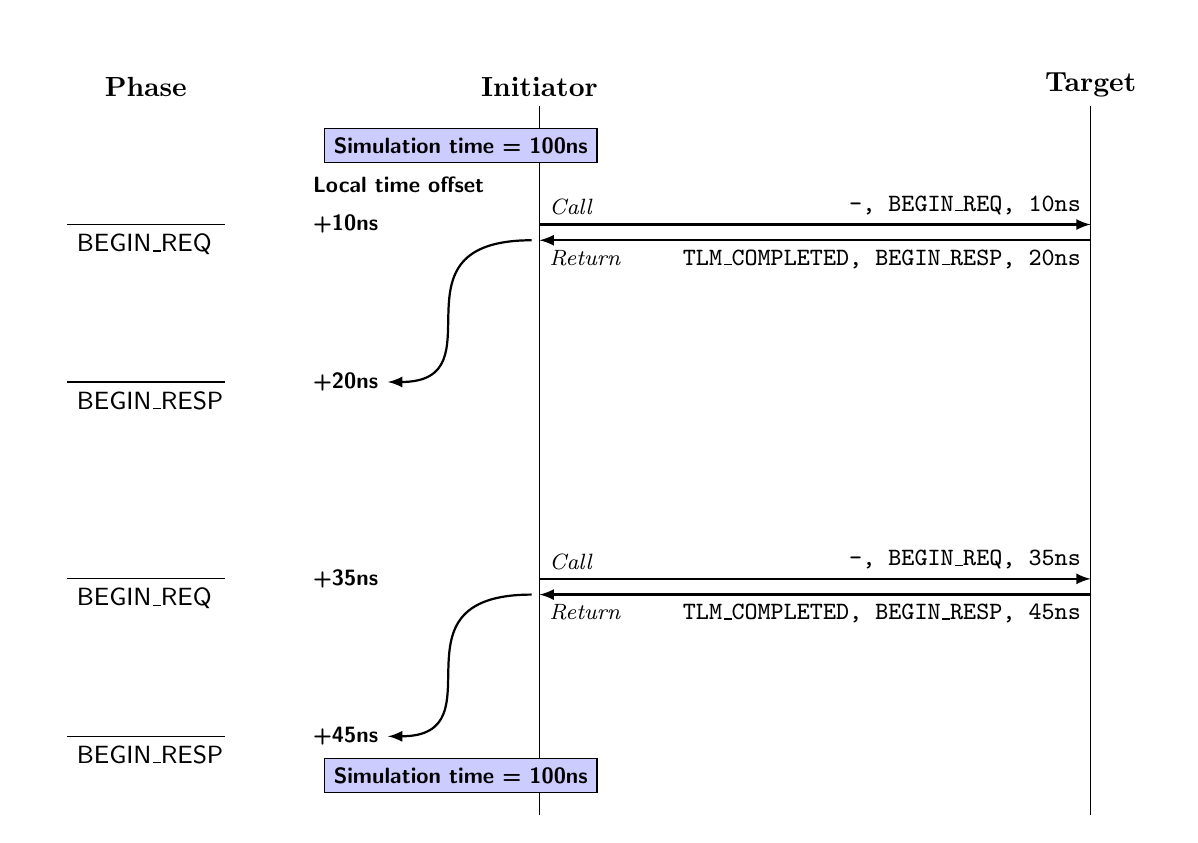
\begin{tikzpicture}
		\clip (0.5,0) rectangle (15,10);
%		\draw[help lines] (0,0) grid (15,10);
		\path (2,9) coordinate (phase);
		\path (1,7.5) coordinate (req0);
		\path (3,7.5) coordinate (req1);
		\path (1,5.5) coordinate (rsp0);
		\path (3,5.5) coordinate (rsp1);
		\path (1,3) coordinate (req1_0);
		\path (3,3) coordinate (req1_1);
		\path (1,1) coordinate (rsp1_0);
		\path (3,1) coordinate (rsp1_1);
		\path (4,8) node(local_time) [right] {\footnotesize \textsf{\textbf{Local time offset}}};
		\path (4,7.5) node(10ns) [right] {\footnotesize \textsf{\textbf{+10ns}}};
		\path (4,5.5) node(20ns) [right] {\footnotesize \textsf{\textbf{+20ns}}};
		\path (4,3) node(35ns) [right] {\footnotesize \textsf{\textbf{+35ns}}};
		\path (4,1) node(45ns) [right] {\footnotesize \textsf{\textbf{+45ns}}};
		\path (7,0) coordinate (llb);
		\path (7,9) coordinate (llt);
		\path (14,0) coordinate (rlb);
		\path (14,9) coordinate (rlt);
		\path (7,7.5) coordinate (call_left);
		\path (14,7.5) coordinate (call_right);
		\path (7,7.3) coordinate (ret_left);
		\path (14,7.3) coordinate (ret_right);
		\path (7,3) coordinate (call2_left);
		\path (14,3) coordinate (call2_right);
		\path (7,2.8) coordinate (ret2_left);
		\path (14,2.8) coordinate (ret2_right);

		\draw (phase) node[above] {\textbf{Phase}};
		\draw (llb) -- (llt)
			node[above] {\textbf{Initiator}};
		\draw (rlb) -- (rlt)
			node[above] {\textbf{Target}};
		\draw (req0) node[below right] {\small \textsf{BEGIN\_REQ}} -- (req1);
		\draw (rsp0) node[below right] {\small \textsf{BEGIN\_RESP}} -- (rsp1);
		\draw (req1_0) node[below right] {\small \textsf{BEGIN\_REQ}} -- (req1_1);
		\draw (rsp1_0) node[below right] {\small \textsf{BEGIN\_RESP}} -- (rsp1_1);
		\draw[thick,-latex] (call_left) -- (call_right);
		\draw (call_left) node[above right] {\footnotesize \emph{Call}};
		\draw (call_right) node[above left] {\small \texttt{\textbf{-, BEGIN\_REQ, 10ns}}};
		\draw[thick,latex-] (ret_left) -- (ret_right);
		\draw (ret_left) node[below right] {\footnotesize \emph{Return}};
		\draw (ret_right) node[below left] {\small \texttt{\textbf{TLM\_COMPLETED, BEGIN\_RESP, 20ns}}};
		\draw[thick,-latex] (call2_left) -- (call2_right);
		\draw (call2_left) node[above right] {\footnotesize \emph{Call}};
		\draw (call2_right) node[above left] {\small \texttt{\textbf{-, BEGIN\_REQ, 35ns}}};
		\draw[thick,latex-] (ret2_left) -- (ret2_right);
		\draw (ret2_left) node[below right] {\footnotesize \emph{Return}};
		\draw (ret2_right) node[below left] {\small \texttt{\textbf{TLM\_COMPLETED, BEGIN\_RESP, 45ns}}};
		\path (6,8.5) node(100ns) [rectangle,draw,fill=blue!20] {\footnotesize \textsf{\textbf{Simulation time = 100ns}}};
		\path (6,0.5) node(100_ns) [rectangle,draw,fill=blue!20] {\footnotesize \textsf{\textbf{Simulation time = 100ns}}};
		\path (ret_left) +(-2,0) coordinate (control_ret_left);
		\path (20ns) +(2,0) coordinate (control_20ns);
		\draw[thick,-latex] (ret_left) +(-0.1,0) .. controls (control_ret_left) and (control_20ns) .. (20ns)[above];
		\path (ret2_left) +(-2,0) coordinate (control_ret2_left);
		\path (45ns) +(2,0) coordinate (control_45ns);
		\draw[thick,-latex] (ret2_left) +(-0.1,0) .. controls (control_ret2_left) and (control_45ns) .. (45ns)[above];
	\end{tikzpicture}
	\end{center}
	\caption{Loosely-timed coding style with temporal decoupling message chart.}
	\label{fig:chart_lt_with_temporal_decoupling}
\end{figure}
}

\clearpage
\subsection{Loosely-timed with temporal decoupling and synchronization-on-demand}

\mode<presentation>{

\begin{frame}
	\frametitle{\scriptsize Loosely-timed with temporal decoupling and synchronization-on-demand}

\begin{figure}[h]
	\begin{center}
	\begin{tikzpicture}[transform shape,scale=0.7]
		\clip (0.5,0) rectangle (15,10);
%		\draw[help lines] (0,0) grid (15,10);
		\path (2,9) coordinate (phase);
		\path (1,7.5) coordinate (req0);
		\path (3,7.5) coordinate (req1);
		\path (1,4) coordinate (rsp0);
		\path (3,4) coordinate (rsp1);
		\path (1,2) coordinate (req1_0);
		\path (3,2) coordinate (req1_1);
		\path (1,1) coordinate (rsp1_0);
		\path (3,1) coordinate (rsp1_1);
		\path (4,8) node(local_time) [right] {\footnotesize \textsf{\textbf{Local time offset}}};
		\path (4,7.5) node(10ns) [right] {\footnotesize \textsf{\textbf{+10ns}}};
		\path (4,6.5) node(wait) [right] {\footnotesize \textsf{\textbf{wait(\ldots)}}};
		\path (4,4) node(0s) [right] {\footnotesize \textsf{\textbf{+0ns}}};
		\path (4,2) node(20ns) [right] {\footnotesize \textsf{\textbf{+20ns}}};
		\path (4,1) node(30ns) [right] {\footnotesize \textsf{\textbf{+30ns}}};
		\path (7,0) coordinate (llb);
		\path (7,9) coordinate (llt);
		\path (14,0) coordinate (rlb);
		\path (14,9) coordinate (rlt);
		\path (7,7.5) coordinate (call_left);
		\path (14,7.5) coordinate (call_right);
		\path (7,7.3) coordinate (ret_left);
		\path (14,7.3) coordinate (ret_right);
		\path (7,4) coordinate (call2_left);
		\path (14,4) coordinate (call2_right);
		\path (7,3.8) coordinate (ret2_left);
		\path (14,3.8) coordinate (ret2_right);
		\path (7,2) coordinate (call3_left);
		\path (14,2) coordinate (call3_right);
		\path (7,1.8) coordinate (ret3_left);
		\path (14,1.8) coordinate (ret3_right);

		\draw (phase) node[above] {\textbf{Phase}};
		\draw (llb) -- (llt)
			node[above] {\textbf{Initiator}};
		\draw (rlb) -- (rlt)
			node[above] {\textbf{Target}};
		\draw (req0) node[below right] {\small \textsf{BEGIN\_REQ}} -- (req1);
		\draw (rsp0) node[below right] {\small \textsf{BEGIN\_RESP}} -- (rsp1);
		\draw (req1_0) node[below right] {\small \textsf{BEGIN\_REQ}} -- (req1_1);
		\draw (rsp1_0) node[below right] {\small \textsf{BEGIN\_RESP}} -- (rsp1_1);
		\draw[thick,-latex] (call_left) -- (call_right);
		\draw (call_left) node[above right] {\footnotesize \emph{Call}};
		\draw (call_right) node[above left] {\small \texttt{\textbf{-, BEGIN\_REQ, 10ns}}};
		\draw[thick,latex-] (ret_left) -- (ret_right);
		\draw (ret_left) node[below right] {\footnotesize \emph{Return}};
		\draw (ret_right) node[below left] {\small \texttt{\textbf{TLM\_ACCEPTED, -, -}}};
		\draw[thick,latex-] (call2_left) -- (call2_right);
		\draw (call2_right) node[above left] {\footnotesize \emph{Call}};
		\draw (call2_left) node[above right] {\small \texttt{\textbf{-, BEGIN\_RESP, 0ns}}};
		\draw[thick,-latex] (ret2_left) -- (ret2_right);
		\draw (ret2_right) node[below left] {\footnotesize \emph{Return}};
		\draw (ret2_left) node[below right] {\small \texttt{\textbf{TLM\_COMPLETED, -, -}}};
		\draw[thick,-latex] (call3_left) -- (call3_right);
		\draw (call3_left) node[above right] {\footnotesize \emph{Call}};
		\draw (call3_right) node[above left] {\small \texttt{\textbf{-, BEGIN\_REQ, 20ns}}};
		\draw[thick,latex-] (ret3_left) -- (ret3_right);
		\draw (ret3_left) +(0,-0.3) node[below right] {\footnotesize \emph{Return}};
		\draw (ret3_right) node[below left] {\small \texttt{\textbf{TLM\_COMPLETED, BEGIN\_RESP, 30ns}}};
		\path (6,8.5) node(5us) [rectangle,draw,fill=blue!20] {\footnotesize \textsf{\textbf{Simulation time = 5us}}};
		\path (6,5.5) node(6us1) [rectangle,draw,fill=blue!20] {\footnotesize \textsf{\textbf{Simulation time = 6us}}};
		\path (6,0.25) node(6us2) [rectangle,draw,fill=blue!20] {\footnotesize \textsf{\textbf{Simulation time = 6us}}};
		\path (ret_left) +(-1.5,0) coordinate (control_ret_left);
		\path (wait) +(1.5,0) coordinate (control_wait);
		\draw[thick,-latex] (ret_left) +(-0.1,0) .. controls (control_ret_left) and (control_wait) .. (wait)[above];
		\path (ret3_left) +(-2,0) coordinate (control_ret3_left);
		\path (45ns) +(2,0) coordinate (control_45ns);
		\draw[thick,-latex] (ret3_left) +(-0.1,0) .. controls (control_ret3_left) and (control_45ns) .. (45ns)[above];
	\end{tikzpicture}
	\end{center}
\end{figure}

\end{frame}

}

\mode<article>{
Figure~\ref{fig:chart_lt_with_temporal_decoupling_and_sync_on_demand} shows the message exchange that occur when using the loosely-timed coding style with temporal decoupling and synchronization-on-demand.

\begin{figure}[h]
	\begin{center}
	\begin{tikzpicture}
		\clip (0.5,0) rectangle (15,10);
%		\draw[help lines] (0,0) grid (15,10);
		\path (2,9) coordinate (phase);
		\path (1,7.5) coordinate (req0);
		\path (3,7.5) coordinate (req1);
		\path (1,4) coordinate (rsp0);
		\path (3,4) coordinate (rsp1);
		\path (1,2) coordinate (req1_0);
		\path (3,2) coordinate (req1_1);
		\path (1,1) coordinate (rsp1_0);
		\path (3,1) coordinate (rsp1_1);
		\path (4,8) node(local_time) [right] {\footnotesize \textsf{\textbf{Local time offset}}};
		\path (4,7.5) node(10ns) [right] {\footnotesize \textsf{\textbf{+10ns}}};
		\path (4,6.5) node(wait) [right] {\footnotesize \textsf{\textbf{wait(\ldots)}}};
		\path (4,4) node(0s) [right] {\footnotesize \textsf{\textbf{+0ns}}};
		\path (4,2) node(20ns) [right] {\footnotesize \textsf{\textbf{+20ns}}};
		\path (4,1) node(30ns) [right] {\footnotesize \textsf{\textbf{+30ns}}};
		\path (7,0) coordinate (llb);
		\path (7,9) coordinate (llt);
		\path (14,0) coordinate (rlb);
		\path (14,9) coordinate (rlt);
		\path (7,7.5) coordinate (call_left);
		\path (14,7.5) coordinate (call_right);
		\path (7,7.3) coordinate (ret_left);
		\path (14,7.3) coordinate (ret_right);
		\path (7,4) coordinate (call2_left);
		\path (14,4) coordinate (call2_right);
		\path (7,3.8) coordinate (ret2_left);
		\path (14,3.8) coordinate (ret2_right);
		\path (7,2) coordinate (call3_left);
		\path (14,2) coordinate (call3_right);
		\path (7,1.8) coordinate (ret3_left);
		\path (14,1.8) coordinate (ret3_right);

		\draw (phase) node[above] {\textbf{Phase}};
		\draw (llb) -- (llt)
			node[above] {\textbf{Initiator}};
		\draw (rlb) -- (rlt)
			node[above] {\textbf{Target}};
		\draw (req0) node[below right] {\small \textsf{BEGIN\_REQ}} -- (req1);
		\draw (rsp0) node[below right] {\small \textsf{BEGIN\_RESP}} -- (rsp1);
		\draw (req1_0) node[below right] {\small \textsf{BEGIN\_REQ}} -- (req1_1);
		\draw (rsp1_0) node[below right] {\small \textsf{BEGIN\_RESP}} -- (rsp1_1);
		\draw[thick,-latex] (call_left) -- (call_right);
		\draw (call_left) node[above right] {\footnotesize \emph{Call}};
		\draw (call_right) node[above left] {\small \texttt{\textbf{-, BEGIN\_REQ, 10ns}}};
		\draw[thick,latex-] (ret_left) -- (ret_right);
		\draw (ret_left) node[below right] {\footnotesize \emph{Return}};
		\draw (ret_right) node[below left] {\small \texttt{\textbf{TLM\_ACCEPTED, -, -}}};
		\draw[thick,latex-] (call2_left) -- (call2_right);
		\draw (call2_right) node[above left] {\footnotesize \emph{Call}};
		\draw (call2_left) node[above right] {\small \texttt{\textbf{-, BEGIN\_RESP, 0ns}}};
		\draw[thick,-latex] (ret2_left) -- (ret2_right);
		\draw (ret2_right) node[below left] {\footnotesize \emph{Return}};
		\draw (ret2_left) node[below right] {\small \texttt{\textbf{TLM\_COMPLETED, -, -}}};
		\draw[thick,-latex] (call3_left) -- (call3_right);
		\draw (call3_left) node[above right] {\footnotesize \emph{Call}};
		\draw (call3_right) node[above left] {\small \texttt{\textbf{-, BEGIN\_REQ, 20ns}}};
		\draw[thick,latex-] (ret3_left) -- (ret3_right);
		\draw (ret3_left) node[below right] {\footnotesize \emph{Return}};
		\draw (ret3_right) node[below left] {\small \texttt{\textbf{TLM\_COMPLETED, BEGIN\_RESP, 30ns}}};
		\path (6,8.5) node(5us) [rectangle,draw,fill=blue!20] {\footnotesize \textsf{\textbf{Simulation time = 5us}}};
		\path (6,5.5) node(6us1) [rectangle,draw,fill=blue!20] {\footnotesize \textsf{\textbf{Simulation time = 6us}}};
		\path (6,0.25) node(6us2) [rectangle,draw,fill=blue!20] {\footnotesize \textsf{\textbf{Simulation time = 6us}}};
		\path (ret_left) +(-1.5,0) coordinate (control_ret_left);
		\path (wait) +(1.5,0) coordinate (control_wait);
		\draw[thick,-latex] (ret_left) +(-0.1,0) .. controls (control_ret_left) and (control_wait) .. (wait)[above];
		\path (ret3_left) +(-2,0) coordinate (control_ret3_left);
		\path (45ns) +(2,0) coordinate (control_45ns);
		\draw[thick,-latex] (ret3_left) +(-0.1,0) .. controls (control_ret3_left) and (control_45ns) .. (45ns)[above];
	\end{tikzpicture}
	\end{center}
	\caption{Loosely-timed coding style with temporal decoupling and synchronization-on-demand message chart.}
	\label{fig:chart_lt_with_temporal_decoupling_and_sync_on_demand}
\end{figure}
}

\clearpage
\subsection{Loosely-timed with temporal decoupling and quantum}

\mode<presentation>{

\begin{frame}
	\frametitle{\small Loosely-timed with temporal decoupling and quantum}

\begin{figure}[h]
	\begin{center}
	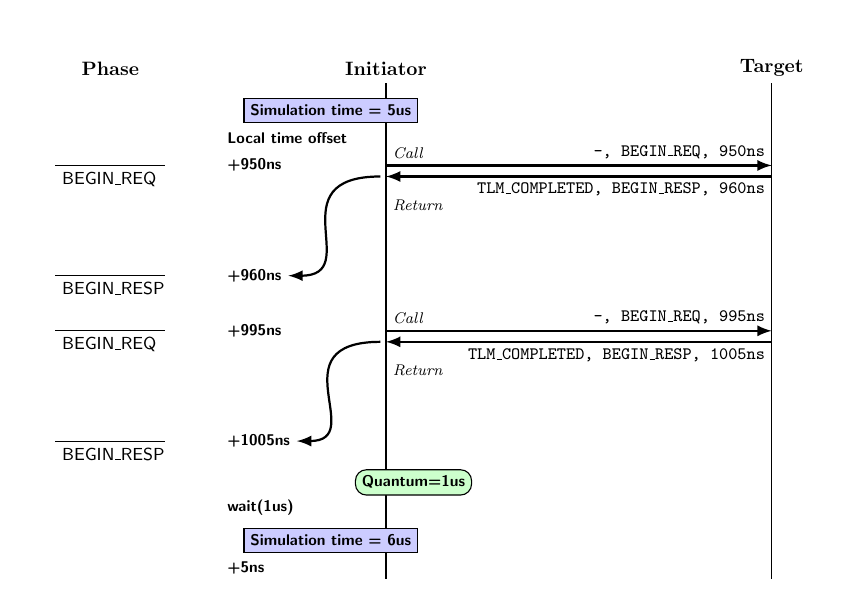
\begin{tikzpicture}[transform shape,scale=0.7]
		\clip (0.5,0) rectangle (15,10);
%		\draw[help lines] (0,0) grid (15,10);
		\path (2,9) coordinate (phase);
		\path (1,7.5) coordinate (req0);
		\path (3,7.5) coordinate (req1);
		\path (1,5.5) coordinate (rsp0);
		\path (3,5.5) coordinate (rsp1);
		\path (1,4.5) coordinate (req1_0);
		\path (3,4.5) coordinate (req1_1);
		\path (1,2.5) coordinate (rsp1_0);
		\path (3,2.5) coordinate (rsp1_1);
		\path (4,8) node(local_time) [right] {\footnotesize \textsf{\textbf{Local time offset}}};
		\path (4,7.5) node(10ns) [right] {\footnotesize \textsf{\textbf{+950ns}}};
		\path (4,5.5) node(20ns) [right] {\footnotesize \textsf{\textbf{+960ns}}};
		\path (4,4.5) node(35ns) [right] {\footnotesize \textsf{\textbf{+995ns}}};
		\path (4,2.5) node(45ns) [right] {\footnotesize \textsf{\textbf{+1005ns}}};
		\path (4,1.3) node(wait) [right] {\footnotesize \textsf{\textbf{wait(1us)}}};
		\path (4,0.2) node(5ns) [right] {\footnotesize \textsf{\textbf{+5ns}}};
		\path (7,0) coordinate (llb);
		\path (7,9) coordinate (llt);
		\path (14,0) coordinate (rlb);
		\path (14,9) coordinate (rlt);
		\path (7,7.5) coordinate (call_left);
		\path (14,7.5) coordinate (call_right);
		\path (7,7.3) coordinate (ret_left);
		\path (14,7.3) coordinate (ret_right);
		\path (7,4.5) coordinate (call2_left);
		\path (14,4.5) coordinate (call2_right);
		\path (7,4.3) coordinate (ret2_left);
		\path (14,4.3) coordinate (ret2_right);

		\draw (phase) node[above] {\textbf{Phase}};
		\draw (llb) -- (llt)
			node[above] {\textbf{Initiator}};
		\draw (rlb) -- (rlt)
			node[above] {\textbf{Target}};
		\draw (req0) node[below right] {\small \textsf{BEGIN\_REQ}} -- (req1);
		\draw (rsp0) node[below right] {\small \textsf{BEGIN\_RESP}} -- (rsp1);
		\draw (req1_0) node[below right] {\small \textsf{BEGIN\_REQ}} -- (req1_1);
		\draw (rsp1_0) node[below right] {\small \textsf{BEGIN\_RESP}} -- (rsp1_1);
		\draw[thick,-latex] (call_left) -- (call_right);
		\draw (call_left) node[above right] {\footnotesize \emph{Call}};
		\draw (call_right) node[above left] {\small \texttt{\textbf{-, BEGIN\_REQ, 950ns}}};
		\draw[thick,latex-] (ret_left) -- (ret_right);
		\draw (ret_left) +(0,-0.3) node[below right] {\footnotesize \emph{Return}};
		\draw (ret_right) node[below left] {\small \texttt{\textbf{TLM\_COMPLETED, BEGIN\_RESP, 960ns}}};
		\draw[thick,-latex] (call2_left) -- (call2_right);
		\draw (call2_left) node[above right] {\footnotesize \emph{Call}};
		\draw (call2_right) node[above left] {\small \texttt{\textbf{-, BEGIN\_REQ, 995ns}}};
		\draw[thick,latex-] (ret2_left) -- (ret2_right);
		\draw (ret2_left) +(0,-0.3) node[below right] {\footnotesize \emph{Return}};
		\draw (ret2_right) node[below left] {\small \texttt{\textbf{TLM\_COMPLETED, BEGIN\_RESP, 1005ns}}};
		\path (6,8.5) node(100ns) [rectangle,draw,fill=blue!20] {\footnotesize \textsf{\textbf{Simulation time = 5us}}};
		\path (6,0.7) node(110ns) [rectangle,draw,fill=blue!20] {\footnotesize \textsf{\textbf{Simulation time = 6us}}};
		\path (7.5,1.75) node(quantum) [rectangle,rounded corners,draw,fill=green!20] {\footnotesize \textsf{\textbf{Quantum=1us}}};
		\path (ret_left) +(-2,0) coordinate (control_ret_left);
		\path (20ns) +(2,0) coordinate (control_20ns);
		\draw[thick,-latex] (ret_left) +(-0.1,0) .. controls (control_ret_left) and (control_20ns) .. (20ns)[above];
		\path (ret2_left) +(-2,0) coordinate (control_ret2_left);
		\path (45ns) +(2,0) coordinate (control_45ns);
		\draw[thick,-latex] (ret2_left) +(-0.1,0) .. controls (control_ret2_left) and (control_45ns) .. (45ns)[above];
	\end{tikzpicture}
	\end{center}
\end{figure}
\end{frame}

}

\mode<article>{
Figure~\ref{fig:chart_lt_with_temporal_decoupling_and_quantum} shows the message exchange that occur when using the loosely-timed coding style and quantum.

\begin{figure}[h]
	\begin{center}
	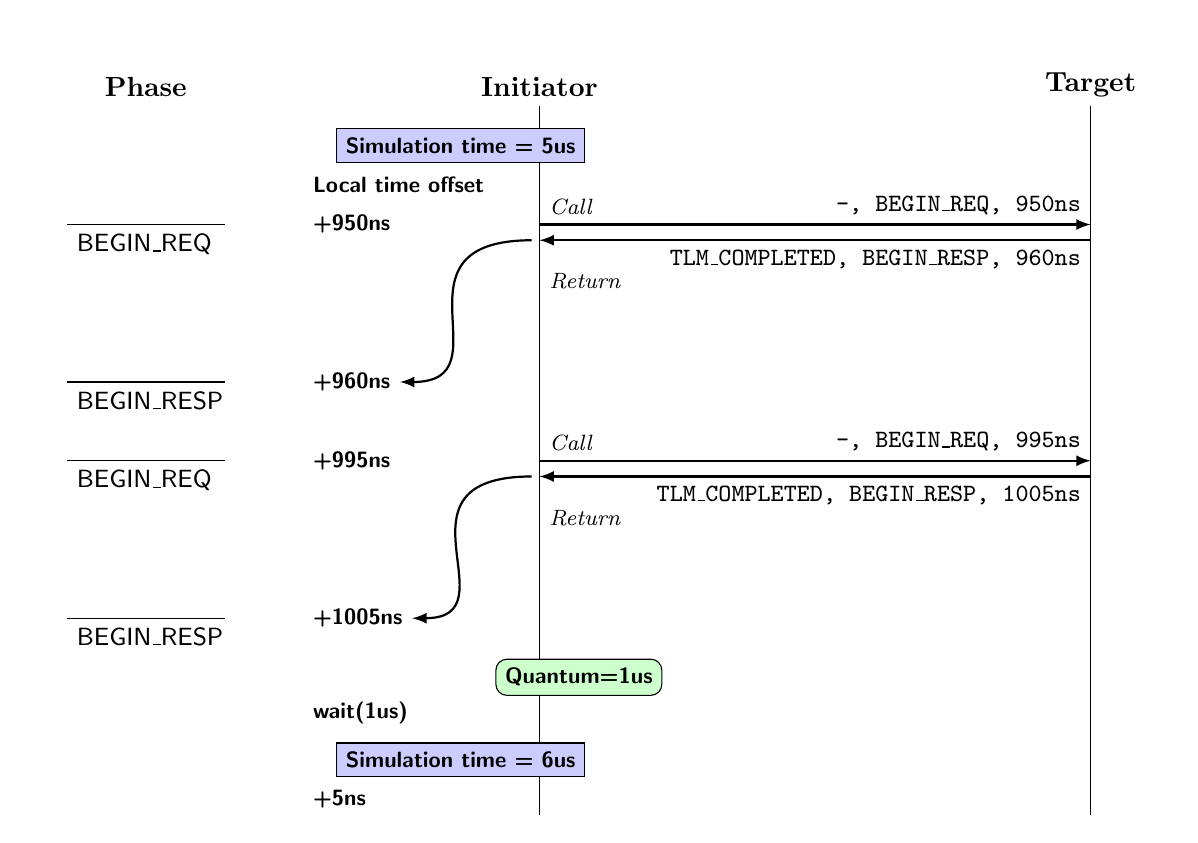
\begin{tikzpicture}
		\clip (0.5,0) rectangle (15,10);
%		\draw[help lines] (0,0) grid (15,10);
		\path (2,9) coordinate (phase);
		\path (1,7.5) coordinate (req0);
		\path (3,7.5) coordinate (req1);
		\path (1,5.5) coordinate (rsp0);
		\path (3,5.5) coordinate (rsp1);
		\path (1,4.5) coordinate (req1_0);
		\path (3,4.5) coordinate (req1_1);
		\path (1,2.5) coordinate (rsp1_0);
		\path (3,2.5) coordinate (rsp1_1);
		\path (4,8) node(local_time) [right] {\footnotesize \textsf{\textbf{Local time offset}}};
		\path (4,7.5) node(10ns) [right] {\footnotesize \textsf{\textbf{+950ns}}};
		\path (4,5.5) node(20ns) [right] {\footnotesize \textsf{\textbf{+960ns}}};
		\path (4,4.5) node(35ns) [right] {\footnotesize \textsf{\textbf{+995ns}}};
		\path (4,2.5) node(45ns) [right] {\footnotesize \textsf{\textbf{+1005ns}}};
		\path (4,1.3) node(wait) [right] {\footnotesize \textsf{\textbf{wait(1us)}}};
		\path (4,0.2) node(5ns) [right] {\footnotesize \textsf{\textbf{+5ns}}};
		\path (7,0) coordinate (llb);
		\path (7,9) coordinate (llt);
		\path (14,0) coordinate (rlb);
		\path (14,9) coordinate (rlt);
		\path (7,7.5) coordinate (call_left);
		\path (14,7.5) coordinate (call_right);
		\path (7,7.3) coordinate (ret_left);
		\path (14,7.3) coordinate (ret_right);
		\path (7,4.5) coordinate (call2_left);
		\path (14,4.5) coordinate (call2_right);
		\path (7,4.3) coordinate (ret2_left);
		\path (14,4.3) coordinate (ret2_right);

		\draw (phase) node[above] {\textbf{Phase}};
		\draw (llb) -- (llt)
			node[above] {\textbf{Initiator}};
		\draw (rlb) -- (rlt)
			node[above] {\textbf{Target}};
		\draw (req0) node[below right] {\small \textsf{BEGIN\_REQ}} -- (req1);
		\draw (rsp0) node[below right] {\small \textsf{BEGIN\_RESP}} -- (rsp1);
		\draw (req1_0) node[below right] {\small \textsf{BEGIN\_REQ}} -- (req1_1);
		\draw (rsp1_0) node[below right] {\small \textsf{BEGIN\_RESP}} -- (rsp1_1);
		\draw[thick,-latex] (call_left) -- (call_right);
		\draw (call_left) node[above right] {\footnotesize \emph{Call}};
		\draw (call_right) node[above left] {\small \texttt{\textbf{-, BEGIN\_REQ, 950ns}}};
		\draw[thick,latex-] (ret_left) -- (ret_right);
		\draw (ret_left) +(0,-0.3) node[below right] {\footnotesize \emph{Return}};
		\draw (ret_right) node[below left] {\small \texttt{\textbf{TLM\_COMPLETED, BEGIN\_RESP, 960ns}}};
		\draw[thick,-latex] (call2_left) -- (call2_right);
		\draw (call2_left) node[above right] {\footnotesize \emph{Call}};
		\draw (call2_right) node[above left] {\small \texttt{\textbf{-, BEGIN\_REQ, 995ns}}};
		\draw[thick,latex-] (ret2_left) -- (ret2_right);
		\draw (ret2_left) +(0,-0.3) node[below right] {\footnotesize \emph{Return}};
		\draw (ret2_right) node[below left] {\small \texttt{\textbf{TLM\_COMPLETED, BEGIN\_RESP, 1005ns}}};
		\path (6,8.5) node(100ns) [rectangle,draw,fill=blue!20] {\footnotesize \textsf{\textbf{Simulation time = 5us}}};
		\path (6,0.7) node(110ns) [rectangle,draw,fill=blue!20] {\footnotesize \textsf{\textbf{Simulation time = 6us}}};
		\path (7.5,1.75) node(quantum) [rectangle,rounded corners,draw,fill=green!20] {\footnotesize \textsf{\textbf{Quantum=1us}}};
		\path (ret_left) +(-2,0) coordinate (control_ret_left);
		\path (20ns) +(2,0) coordinate (control_20ns);
		\draw[thick,-latex] (ret_left) +(-0.1,0) .. controls (control_ret_left) and (control_20ns) .. (20ns)[above];
		\path (ret2_left) +(-2,0) coordinate (control_ret2_left);
		\path (45ns) +(2,0) coordinate (control_45ns);
		\draw[thick,-latex] (ret2_left) +(-0.1,0) .. controls (control_ret2_left) and (control_45ns) .. (45ns)[above];
	\end{tikzpicture}
	\end{center}
	\caption{Loosely-timed coding style with temporal decoupling and quantum message chart.}
	\label{fig:chart_lt_with_temporal_decoupling_and_quantum}
\end{figure}
}

\clearpage
\subsection{Approximately-timed using backward path}

\mode<presentation>{

\begin{frame}
	\frametitle{Approximately-timed using backward path}

\begin{figure}[h]
	\begin{center}
	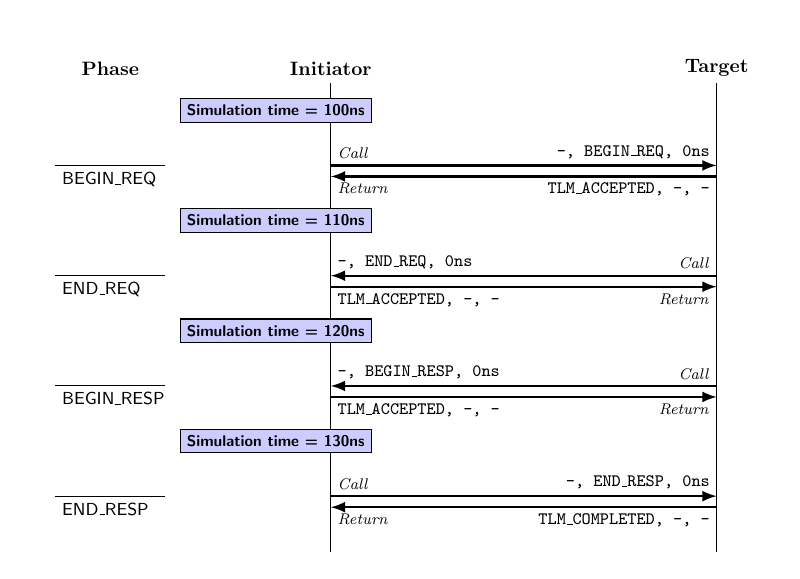
\begin{tikzpicture}[transform shape,scale=0.7]
		\clip (1.5,10.5) rectangle (15,20);
%		\draw[help lines] (0,0) grid (15,20);
		\path (3,19) coordinate (phase);
		\path (7,0) coordinate (llb);
		\path (7,19) coordinate (llt);
		\path (14,0) coordinate (rlb);
		\path (14,19) coordinate (rlt);
		
		\path (6,18.5) coordinate (100ns);
		\path (2,17.5) coordinate (breq_l);
		\path (4,17.5) coordinate (breq_r);
		\path (7,17.5) coordinate (breq_call_l);
		\path (14,17.5) coordinate (breq_call_r);
		\path (7,17.3) coordinate (breq_ret_l);
		\path (14,17.3) coordinate (breq_ret_r);

		\path (6,16.5) coordinate (110ns);
		\path (2,15.5) coordinate (ereq_l);
		\path (4,15.5) coordinate (ereq_r);
		\path (7,15.5) coordinate (ereq_call_l);
		\path (14,15.5) coordinate (ereq_call_r);
		\path (7, 15.3) coordinate (ereq_ret_l);
		\path (14,15.3) coordinate (ereq_ret_r);

		\path (6,14.5) coordinate (120ns);
		\path (2,13.5) coordinate (bresp_l);
		\path (4,13.5) coordinate (bresp_r);
		\path (7,13.5) coordinate (bresp_call_l);
		\path (14,13.5) coordinate (bresp_call_r);
		\path (7,13.3) coordinate (bresp_ret_l);
		\path (14,13.3) coordinate (bresp_ret_r);

		\path (6,12.5) coordinate (130ns);
		\path (2,11.5) coordinate (eresp_l);
		\path (4,11.5) coordinate (eresp_r);
		\path (7,11.5) coordinate (eresp_call_l);
		\path (14,11.5) coordinate (eresp_call_r);
		\path (7,11.3) coordinate (eresp_ret_l);
		\path (14,11.3) coordinate (eresp_ret_r);

		\draw (phase) node[above] {\textbf{Phase}};
		\draw (llb) -- (llt)
			node[above] {\textbf{Initiator}};
		\draw (rlb) -- (rlt)
			node[above] {\textbf{Target}};

		\draw (100ns) node [rectangle,draw,fill=blue!20] {\footnotesize \textsf{\textbf{Simulation time = 100ns}}};
		\draw (breq_l) node[below right] {\small \textsf{BEGIN\_REQ}} -- (breq_r);
		\draw[thick,-latex] (breq_call_l) -- (breq_call_r);
		\draw (breq_call_l) node[above right] {\footnotesize \emph{Call}};
		\draw (breq_call_r) node[above left] {\small \texttt{\textbf{-, BEGIN\_REQ, 0ns}}};
		\draw[thick,latex-] (breq_ret_l) -- (breq_ret_r);
		\draw (breq_ret_l) node[below right] {\footnotesize \emph{Return}};
		\draw (breq_ret_r) node[below left] {\small \texttt{\textbf{TLM\_ACCEPTED, -, -}}};

		\draw (110ns) node [rectangle,draw,fill=blue!20] {\footnotesize \textsf{\textbf{Simulation time = 110ns}}};
		\draw (ereq_l) node[below right] {\small \textsf{END\_REQ}} -- (ereq_r);
		\draw[thick,latex-] (ereq_call_l) -- (ereq_call_r);
		\draw (ereq_call_r) node[above left] {\footnotesize \emph{Call}};
		\draw (ereq_call_l) node[above right] {\small \texttt{\textbf{-, END\_REQ, 0ns}}};
		\draw[thick,-latex] (ereq_ret_l) -- (ereq_ret_r);
		\draw (ereq_ret_r) node[below left] {\footnotesize \emph{Return}};
		\draw (ereq_ret_l) node[below right] {\small \texttt{\textbf{TLM\_ACCEPTED, -, -}}};

		\draw (120ns) node [rectangle,draw,fill=blue!20] {\footnotesize \textsf{\textbf{Simulation time = 120ns}}};
		\draw (bresp_l) node[below right] {\small \textsf{BEGIN\_RESP}} -- (bresp_r);
		\draw[thick,latex-] (bresp_call_l) -- (bresp_call_r);
		\draw (bresp_call_r) node[above left] {\footnotesize \emph{Call}};
		\draw (bresp_call_l) node[above right] {\small \texttt{\textbf{-, BEGIN\_RESP, 0ns}}};
		\draw[thick,-latex] (bresp_ret_l) -- (bresp_ret_r);
		\draw (bresp_ret_r) node[below left] {\footnotesize \emph{Return}};
		\draw (bresp_ret_l) node[below right] {\small \texttt{\textbf{TLM\_ACCEPTED, -, -}}};

		\draw (130ns) node [rectangle,draw,fill=blue!20] {\footnotesize \textsf{\textbf{Simulation time = 130ns}}};
		\draw (eresp_l) node[below right] {\small \textsf{END\_RESP}} -- (eresp_r);
		\draw[thick,-latex] (eresp_call_l) -- (eresp_call_r);
		\draw (eresp_call_l) node[above right] {\footnotesize \emph{Call}};
		\draw (eresp_call_r) node[above left] {\small \texttt{\textbf{-, END\_RESP, 0ns}}};
		\draw[thick,latex-] (eresp_ret_l) -- (eresp_ret_r);
		\draw (eresp_ret_l) node[below right] {\footnotesize \emph{Return}};
		\draw (eresp_ret_r) node[below left] {\small \texttt{\textbf{TLM\_COMPLETED, -, -}}};

	\end{tikzpicture}
	\end{center}
\end{figure}


\end{frame}

}

\mode<article>{
Figure~\ref{fig:chart_at_using_backward_path} shows the message exchange that occur when using the approximately-timed coding style using the backward path.

\begin{figure}[h]
	\begin{center}
	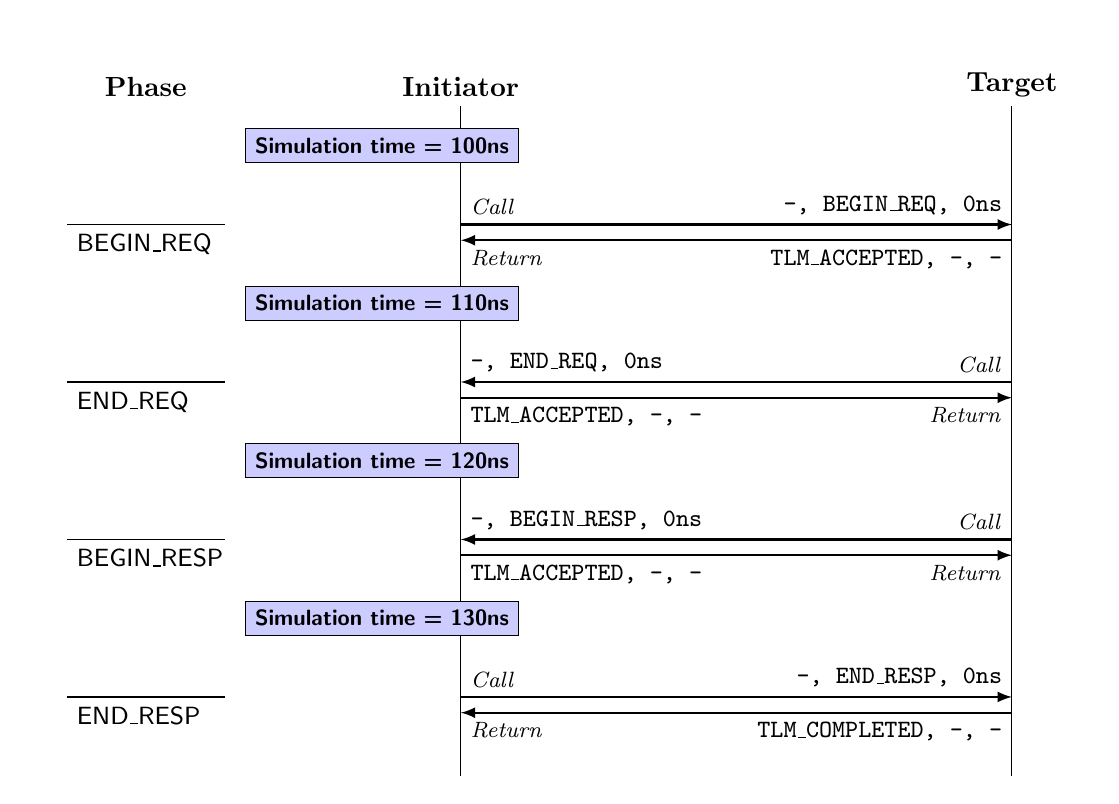
\begin{tikzpicture}
		\clip (1.5,10.5) rectangle (15,20);
%		\draw[help lines] (0,0) grid (15,20);
		\path (3,19) coordinate (phase);
		\path (7,0) coordinate (llb);
		\path (7,19) coordinate (llt);
		\path (14,0) coordinate (rlb);
		\path (14,19) coordinate (rlt);
		
		\path (6,18.5) coordinate (100ns);
		\path (2,17.5) coordinate (breq_l);
		\path (4,17.5) coordinate (breq_r);
		\path (7,17.5) coordinate (breq_call_l);
		\path (14,17.5) coordinate (breq_call_r);
		\path (7,17.3) coordinate (breq_ret_l);
		\path (14,17.3) coordinate (breq_ret_r);

		\path (6,16.5) coordinate (110ns);
		\path (2,15.5) coordinate (ereq_l);
		\path (4,15.5) coordinate (ereq_r);
		\path (7,15.5) coordinate (ereq_call_l);
		\path (14,15.5) coordinate (ereq_call_r);
		\path (7, 15.3) coordinate (ereq_ret_l);
		\path (14,15.3) coordinate (ereq_ret_r);

		\path (6,14.5) coordinate (120ns);
		\path (2,13.5) coordinate (bresp_l);
		\path (4,13.5) coordinate (bresp_r);
		\path (7,13.5) coordinate (bresp_call_l);
		\path (14,13.5) coordinate (bresp_call_r);
		\path (7,13.3) coordinate (bresp_ret_l);
		\path (14,13.3) coordinate (bresp_ret_r);

		\path (6,12.5) coordinate (130ns);
		\path (2,11.5) coordinate (eresp_l);
		\path (4,11.5) coordinate (eresp_r);
		\path (7,11.5) coordinate (eresp_call_l);
		\path (14,11.5) coordinate (eresp_call_r);
		\path (7,11.3) coordinate (eresp_ret_l);
		\path (14,11.3) coordinate (eresp_ret_r);

		\draw (phase) node[above] {\textbf{Phase}};
		\draw (llb) -- (llt)
			node[above] {\textbf{Initiator}};
		\draw (rlb) -- (rlt)
			node[above] {\textbf{Target}};

		\draw (100ns) node [rectangle,draw,fill=blue!20] {\footnotesize \textsf{\textbf{Simulation time = 100ns}}};
		\draw (breq_l) node[below right] {\small \textsf{BEGIN\_REQ}} -- (breq_r);
		\draw[thick,-latex] (breq_call_l) -- (breq_call_r);
		\draw (breq_call_l) node[above right] {\footnotesize \emph{Call}};
		\draw (breq_call_r) node[above left] {\small \texttt{\textbf{-, BEGIN\_REQ, 0ns}}};
		\draw[thick,latex-] (breq_ret_l) -- (breq_ret_r);
		\draw (breq_ret_l) node[below right] {\footnotesize \emph{Return}};
		\draw (breq_ret_r) node[below left] {\small \texttt{\textbf{TLM\_ACCEPTED, -, -}}};

		\draw (110ns) node [rectangle,draw,fill=blue!20] {\footnotesize \textsf{\textbf{Simulation time = 110ns}}};
		\draw (ereq_l) node[below right] {\small \textsf{END\_REQ}} -- (ereq_r);
		\draw[thick,latex-] (ereq_call_l) -- (ereq_call_r);
		\draw (ereq_call_r) node[above left] {\footnotesize \emph{Call}};
		\draw (ereq_call_l) node[above right] {\small \texttt{\textbf{-, END\_REQ, 0ns}}};
		\draw[thick,-latex] (ereq_ret_l) -- (ereq_ret_r);
		\draw (ereq_ret_r) node[below left] {\footnotesize \emph{Return}};
		\draw (ereq_ret_l) node[below right] {\small \texttt{\textbf{TLM\_ACCEPTED, -, -}}};

		\draw (120ns) node [rectangle,draw,fill=blue!20] {\footnotesize \textsf{\textbf{Simulation time = 120ns}}};
		\draw (bresp_l) node[below right] {\small \textsf{BEGIN\_RESP}} -- (bresp_r);
		\draw[thick,latex-] (bresp_call_l) -- (bresp_call_r);
		\draw (bresp_call_r) node[above left] {\footnotesize \emph{Call}};
		\draw (bresp_call_l) node[above right] {\small \texttt{\textbf{-, BEGIN\_RESP, 0ns}}};
		\draw[thick,-latex] (bresp_ret_l) -- (bresp_ret_r);
		\draw (bresp_ret_r) node[below left] {\footnotesize \emph{Return}};
		\draw (bresp_ret_l) node[below right] {\small \texttt{\textbf{TLM\_ACCEPTED, -, -}}};

		\draw (130ns) node [rectangle,draw,fill=blue!20] {\footnotesize \textsf{\textbf{Simulation time = 130ns}}};
		\draw (eresp_l) node[below right] {\small \textsf{END\_RESP}} -- (eresp_r);
		\draw[thick,-latex] (eresp_call_l) -- (eresp_call_r);
		\draw (eresp_call_l) node[above right] {\footnotesize \emph{Call}};
		\draw (eresp_call_r) node[above left] {\small \texttt{\textbf{-, END\_RESP, 0ns}}};
		\draw[thick,latex-] (eresp_ret_l) -- (eresp_ret_r);
		\draw (eresp_ret_l) node[below right] {\footnotesize \emph{Return}};
		\draw (eresp_ret_r) node[below left] {\small \texttt{\textbf{TLM\_COMPLETED, -, -}}};

	\end{tikzpicture}
	\end{center}
	\caption{Approximately-timed coding style using backward message chart.}
	\label{fig:chart_at_using_backward_path}
\end{figure}
}

\clearpage
\subsection{Approximately-timed with timing annotation}

\mode<presentation>{

\begin{frame}
	\frametitle{Approximately-timed with timing annotation}

\begin{figure}[h]
	\begin{center}
	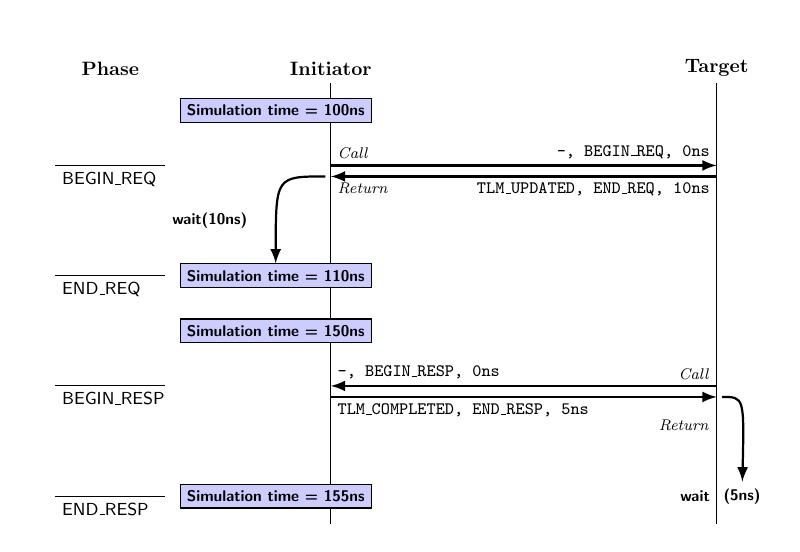
\begin{tikzpicture}[transform shape,scale=0.7]
		\clip (1.5,11) rectangle (15,20);
%		\draw[help lines] (0,0) grid (16,20);
		\path (3,19) coordinate (phase);
		\path (7,0) coordinate (llb);
		\path (7,19) coordinate (llt);
		\path (14,0) coordinate (rlb);
		\path (14,19) coordinate (rlt);
		
		\path (6,18.5) coordinate (100ns);
		\path (2,17.5) coordinate (breq_l);
		\path (4,17.5) coordinate (breq_r);
		\path (7,17.5) coordinate (breq_call_l);
		\path (14,17.5) coordinate (breq_call_r);
		\path (7,17.3) coordinate (breq_ret_l);
		\path (14,17.3) coordinate (breq_ret_r);
		
		\path (4,16.5) coordinate (wait10ns);

		\path (6,15.5) coordinate (110ns);
		\path (2,15.5) coordinate (ereq_l);
		\path (4,15.5) coordinate (ereq_r);

		\path (6,14.5) coordinate (150ns);
		\path (2,13.5) coordinate (bresp_l);
		\path (4,13.5) coordinate (bresp_r);
		\path (7,13.5) coordinate (bresp_call_l);
		\path (14,13.5) coordinate (bresp_call_r);
		\path (7,13.3) coordinate (bresp_ret_l);
		\path (14,13.3) coordinate (bresp_ret_r);

		\path (6,11.5) coordinate (155ns);
		\path (2,11.5) coordinate (eresp_l);
		\path (4,11.5) coordinate (eresp_r);
		\path (14,11.5) coordinate (wait5ns);

		\draw (phase) node[above] {\textbf{Phase}};
		\draw (llb) -- (llt)
			node[above] {\textbf{Initiator}};
		\draw (rlb) -- (rlt)
			node[above] {\textbf{Target}};

		\draw (100ns) node [rectangle,draw,fill=blue!20] {\footnotesize \textsf{\textbf{Simulation time = 100ns}}};
		\draw (breq_l) node[below right] {\small \textsf{BEGIN\_REQ}} -- (breq_r);
		\draw[thick,-latex] (breq_call_l) -- (breq_call_r);
		\draw (breq_call_l) node[above right] {\footnotesize \emph{Call}};
		\draw (breq_call_r) node[above left] {\small \texttt{\textbf{-, BEGIN\_REQ, 0ns}}};
		\draw[thick,latex-] (breq_ret_l) -- (breq_ret_r);
		\draw (breq_ret_l) node[below right] {\footnotesize \emph{Return}};
		\draw (breq_ret_r) node[below left] {\small \texttt{\textbf{TLM\_UPDATED, END\_REQ, 10ns}}};

		\draw (wait10ns) node(wait10ns_rect) [right] {\footnotesize \textsf{\textbf{wait(10ns)}}};
		
		\draw (110ns) node(sim110ns) [rectangle,draw,fill=blue!20] {\footnotesize \textsf{\textbf{Simulation time = 110ns}}};
		\path (breq_ret_l) +(-1,0) coordinate (control);
		\draw[thick,-latex] (breq_ret_l) +(-0.1,0) .. controls (control) .. (sim110ns)[above];

		\draw (ereq_l) node[below right] {\small \textsf{END\_REQ}} -- (ereq_r);

		\draw (150ns) node [rectangle,draw,fill=blue!20] {\footnotesize \textsf{\textbf{Simulation time = 150ns}}};
		\draw (bresp_l) node[below right] {\small \textsf{BEGIN\_RESP}} -- (bresp_r);
		\draw[thick,latex-] (bresp_call_l) -- (bresp_call_r);
		\draw (bresp_call_r) node[above left] {\footnotesize \emph{Call}};
		\draw (bresp_call_l) node[above right] {\small \texttt{\textbf{-, BEGIN\_RESP, 0ns}}};
		\draw[thick,-latex] (bresp_ret_l) -- (bresp_ret_r);
		\draw (bresp_ret_r) +(0,-0.3) node[below left] {\footnotesize \emph{Return}};
		\draw (bresp_ret_l) node[below right] {\small \texttt{\textbf{TLM\_COMPLETED, END\_RESP, 5ns}}};

		\draw (155ns) node [rectangle,draw,fill=blue!20] {\footnotesize \textsf{\textbf{Simulation time = 155ns}}};
		\draw (eresp_l) node[below right] {\small \textsf{END\_RESP}} -- (eresp_r);

		\draw (wait5ns) node [left] {\footnotesize \textsf{\textbf{wait}}};
		\draw (wait5ns) node(wait5ns_rect) [right] {\footnotesize \textsf{\textbf{(5ns)}}};
		\path (bresp_ret_r) +(0.5,0) coordinate (control);
		\draw[thick,-latex] (bresp_ret_r) +(0.1,0) .. controls (control) .. (wait5ns_rect)[above];
	\end{tikzpicture}
	\end{center}
\end{figure}

\end{frame}

}

\mode<article>{
Figure~\ref{fig:chart_at_with_timing_annotation} shows the message exchange that occur when using the approximately-timed coding style with timing annotations.

\begin{figure}[h]
	\begin{center}
	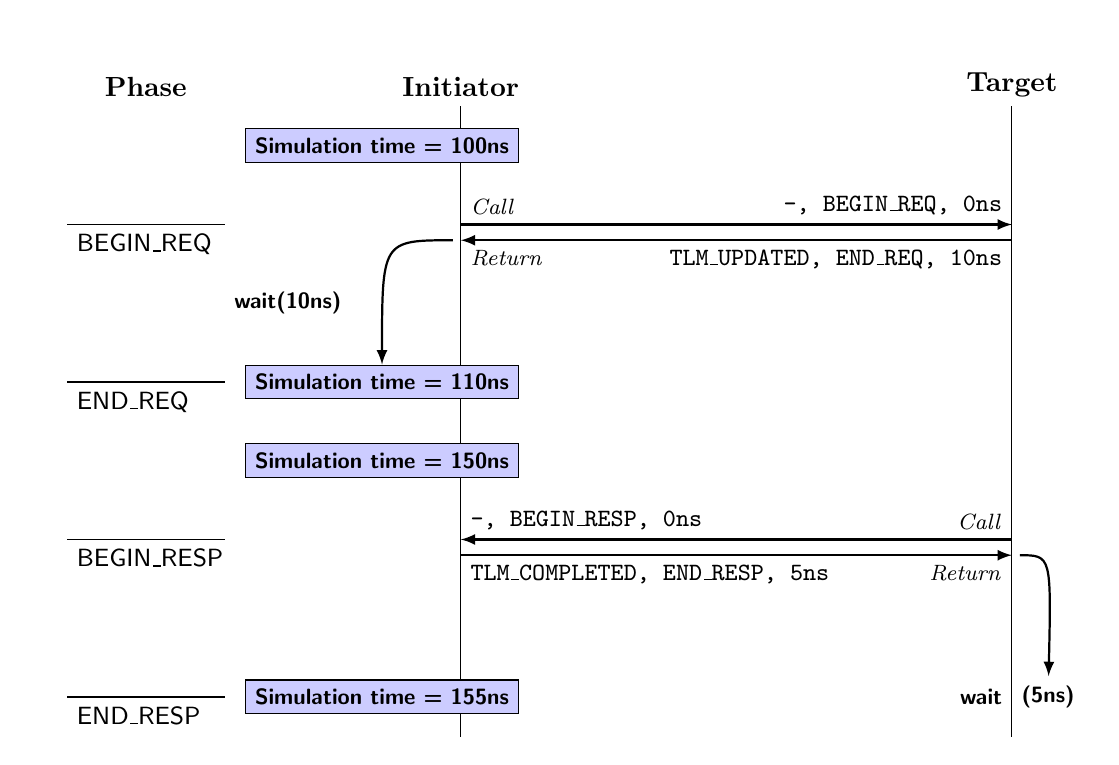
\begin{tikzpicture}
		\clip (1.5,11) rectangle (15,20);
%		\draw[help lines] (0,0) grid (16,20);
		\path (3,19) coordinate (phase);
		\path (7,0) coordinate (llb);
		\path (7,19) coordinate (llt);
		\path (14,0) coordinate (rlb);
		\path (14,19) coordinate (rlt);
		
		\path (6,18.5) coordinate (100ns);
		\path (2,17.5) coordinate (breq_l);
		\path (4,17.5) coordinate (breq_r);
		\path (7,17.5) coordinate (breq_call_l);
		\path (14,17.5) coordinate (breq_call_r);
		\path (7,17.3) coordinate (breq_ret_l);
		\path (14,17.3) coordinate (breq_ret_r);
		
		\path (4,16.5) coordinate (wait10ns);

		\path (6,15.5) coordinate (110ns);
		\path (2,15.5) coordinate (ereq_l);
		\path (4,15.5) coordinate (ereq_r);

		\path (6,14.5) coordinate (150ns);
		\path (2,13.5) coordinate (bresp_l);
		\path (4,13.5) coordinate (bresp_r);
		\path (7,13.5) coordinate (bresp_call_l);
		\path (14,13.5) coordinate (bresp_call_r);
		\path (7,13.3) coordinate (bresp_ret_l);
		\path (14,13.3) coordinate (bresp_ret_r);

		\path (6,11.5) coordinate (155ns);
		\path (2,11.5) coordinate (eresp_l);
		\path (4,11.5) coordinate (eresp_r);
		\path (14,11.5) coordinate (wait5ns);

		\draw (phase) node[above] {\textbf{Phase}};
		\draw (llb) -- (llt)
			node[above] {\textbf{Initiator}};
		\draw (rlb) -- (rlt)
			node[above] {\textbf{Target}};

		\draw (100ns) node [rectangle,draw,fill=blue!20] {\footnotesize \textsf{\textbf{Simulation time = 100ns}}};
		\draw (breq_l) node[below right] {\small \textsf{BEGIN\_REQ}} -- (breq_r);
		\draw[thick,-latex] (breq_call_l) -- (breq_call_r);
		\draw (breq_call_l) node[above right] {\footnotesize \emph{Call}};
		\draw (breq_call_r) node[above left] {\small \texttt{\textbf{-, BEGIN\_REQ, 0ns}}};
		\draw[thick,latex-] (breq_ret_l) -- (breq_ret_r);
		\draw (breq_ret_l) node[below right] {\footnotesize \emph{Return}};
		\draw (breq_ret_r) node[below left] {\small \texttt{\textbf{TLM\_UPDATED, END\_REQ, 10ns}}};

		\draw (wait10ns) node(wait10ns_rect) [right] {\footnotesize \textsf{\textbf{wait(10ns)}}};
		
		\draw (110ns) node(sim110ns) [rectangle,draw,fill=blue!20] {\footnotesize \textsf{\textbf{Simulation time = 110ns}}};
		\path (breq_ret_l) +(-1,0) coordinate (control);
		\draw[thick,-latex] (breq_ret_l) +(-0.1,0) .. controls (control) .. (sim110ns)[above];

		\draw (ereq_l) node[below right] {\small \textsf{END\_REQ}} -- (ereq_r);

		\draw (150ns) node [rectangle,draw,fill=blue!20] {\footnotesize \textsf{\textbf{Simulation time = 150ns}}};
		\draw (bresp_l) node[below right] {\small \textsf{BEGIN\_RESP}} -- (bresp_r);
		\draw[thick,latex-] (bresp_call_l) -- (bresp_call_r);
		\draw (bresp_call_r) node[above left] {\footnotesize \emph{Call}};
		\draw (bresp_call_l) node[above right] {\small \texttt{\textbf{-, BEGIN\_RESP, 0ns}}};
		\draw[thick,-latex] (bresp_ret_l) -- (bresp_ret_r);
		\draw (bresp_ret_r) node[below left] {\footnotesize \emph{Return}};
		\draw (bresp_ret_l) node[below right] {\small \texttt{\textbf{TLM\_COMPLETED, END\_RESP, 5ns}}};

		\draw (155ns) node [rectangle,draw,fill=blue!20] {\footnotesize \textsf{\textbf{Simulation time = 155ns}}};
		\draw (eresp_l) node[below right] {\small \textsf{END\_RESP}} -- (eresp_r);

		\draw (wait5ns) node [left] {\footnotesize \textsf{\textbf{wait}}};
		\draw (wait5ns) node(wait5ns_rect) [right] {\footnotesize \textsf{\textbf{(5ns)}}};
		\path (bresp_ret_r) +(0.5,0) coordinate (control);
		\draw[thick,-latex] (bresp_ret_r) +(0.1,0) .. controls (control) .. (wait5ns_rect)[above];
	\end{tikzpicture}
	\end{center}
	\caption{Approximately-timed coding style with timing annotation message chart.}
	\label{fig:chart_at_with_timing_annotation}
\end{figure}
}

% to do if we have time
% \subsection{Loosely- to approximately-timed adapter}

% to do if we have time
% \subsection{Approximately-timed initiator to loosely-timed target}


\mode<article>{
	\clearpage
}

\section{Other things}

\mode<presentation>{
\begin{frame}
	\frametitle{Other things}
	\begin{itemize}
		\item Things appearing in the current TLM 2.0 revision:
		\begin{itemize}
			\item Analysis interface and analysis ports.
			\item Adapters examples.
			\item Generic payload extension mechanism.
		\end{itemize}
		\item Things missing in the current TLM 2.0 revision:
		\begin{itemize}
			\item New standard protocols.
			\item Atomic transactions.
		\end{itemize}
	\end{itemize}
\end{frame}
}

\mode<article>{
In this tutorial we have learn the basics of TLM 2.0, but still some things remain if you really want to learn all about TLM 2.0. 
For example:
\begin{itemize}
	\item we have not talked about the analysis interface and analysis ports.
	They are intended to support the distribution of transactions to multiple 
components for analysis, meaning tasks such as checking for functional correctness or collecting functional coverage statistics.
	\item we have not seen examples on how to connect modules using different coding styles or TLM modules with cycle level modules. 
	Those are called adapters, and the TLM 2.0 provides some examples on how this can be done. 
	Usually it is done with a module that translates (the adapter) the coding style of the initiator module with the coding style of the second module.
	\item you have seen that the generic payload could be extended, however we have not talked about this because it could be considered as a non basic feature. 
	Again, the TLM 2.0 user manual explains how this can be done. 
\end{itemize}

There are even some things that the TLM 2.0 proposed standard does not explain. 
For example, new protocols (e.g., interrupts) can appear in future version of the standard.
Also the TLM 2.0 user manual explicitly states that the other capabilities like the atomic transactions might appear in future revisions of the Accellera TLM.

}


\input{tlm/exercise}


\newpage

\mode<article>{
\chapter{SystemC TLM 2.0}
}

\mode<presentation>{
\part{SystemC TLM 2.0}
}

\mode<presentation>{
\begin{frame}
	\frametitle{VP4: SystemC TLM 2.0}
	\begin{block}{Accelera SystemC TLM 2.0}
		The Transaction Level Modeling standard of Accelera (previously the Open SystemC Initiative - OSCI).
	\end{block}
	\begin{itemize}
		\item<1-> Introduction
		\item<1-> Interfaces
		\item<1-> Sockets
		\item<1-> Temporal decoupling and the Quantum Keeper
		\item<1-> The Generic Payload
	\end{itemize}
\end{frame}
}

\subsection {Eléments de contexte}
Au cours de mon cursus à l'Ecole d'ingénieur Denis Diderot, j'ai eu l'occasion d'effectuer un stage de 6 mois entre la 2 ième et 3 ième année. 
J'ai donc choisi d'effectuer ce stage au C.E.A List afin d'avoir une expérience professionelle dans un organisme de recherche en informatique et de développer de nouvelles connaissances dans le domaine des systèmes embarqués.
Ma formation étant spécialisé dans la conception de logiciels embarqués et ayant suivi des cours d'architecture des processeurs, 
j'ai pensé qu'il serai intéressant d'approfondir mes connaissances dans le fonctionnenent des processeur afin d'avoir une vision plus complète de l'éxecution des programmes (niveau assembleur).
Gilles Mouchard et Reda Nouacer de l'équipe UNISIM recherchaient un étudiant afin d'effectuer un stage de 6 mois consistant à réaliser un simulateur de jeu d'instruction (ISS) d'un proceseur embarqué. 
\subsection{Contenue du document}
Ce document décrit le travail réalisé au cours de ce stage pendant la période du 10 mars au 31 août 2014 au sein du laboratoire LSL du CEA LIST.
Après une brève présentation du laboratoire et de l'équipe, j'établirai un  état de l'art sur les méthodes de conception et validation d'un simulateur suivie la présentation des outils utilisés pour le projet.
Puis je décrirai les étapes de réalisation et les résulats obtenues sur le processeur choisie par l'équipe.
J'évoquerai également les problèmes rencontrés et les moyens pour les résoudre. 
Enfin j'établirai un bilan sur les connaissances acquises durant ce stage concernant la simulation mais aussi plus généralement sur les méthodes de développement de logiciel.      

\mode<article>{
	\clearpage
}

\section{Interfaces}

\mode<presentation>{
\begin{frame}
	\frametitle{Core TLM2 interfaces}
	\begin{block}{Definition}
		An interface is the way modules use to communicate between each
		other.
	\end{block}
	\begin{itemize}
		\item<1-> TLM2 keeps the core interfaces from TLM1.
		\item<1-> TLM2 adds the following interfaces:
		\begin{itemize}
			\item<1-> blocking and non-blocking transport interfaces,
			\item<1-> a direct memory interface (DMI), and
			\item<1-> a debug transaction interface.
		\end{itemize}
	\end{itemize}
\end{frame}
}

\mode<article>{
As we have seen for Cycle Level Modeling modules used ports to communicate with each other.
With Transaction Level Modeling modules still use ports, however they are quite different.
Ports under TLM are attached to interfaces, those are methods that are implemented by the target module.
TLM2 defines a series of interfaces that the programmer can use to implement his/her TLM simulator.

TLM2 for compatibility issues kept the interfaces defined by TLM1, so previous simulators using TLM1 interfaces could be used with the new TLM definition.
However, the TLM Accellera working group recommends to build new modules using TLM2 interfaces and writing rules.
For this reason we are not going to explain TLM1 interfaces and focus only on the new TLM2 interfaces.

In the following subsections the TLM2 interfaces will be introduced in detail:
\begin{itemize}
	\item the blocking transport interface,
	\item the non-blocking transport interface,
	\item the direct memory interface (DMI), and
	\item the debug transaction interface.
\end{itemize}
}

\subsection{Blocking transport interface}

\mode<presentation>{
\begin{frame}
	\frametitle{Blocking transport interface}
	\setbeamercolor{postit}{fg=black,bg=yellow}
	\begin{beamercolorbox}[center,rounded=true,wd=\textwidth]{postit}
		Designed for the untimed and loosely-timed coding style.
	\end{beamercolorbox}
	\begin{itemize}
		\item<1->Definition:
	\begin{figure}[h]
		\lstinputlisting{tlm/b_transport.cc}
	\end{figure}
		\item<2->The \texttt\textbf{TRANS} argument is by default set to \texttt{\textbf{tlm\_generic\_payload}}.
		\item<3->Recommended to use the generic payload for interoperability issues.
		\item<4->\texttt{sc\_time} parameter: precise simulation time (relative to the last synchronization) the call is taking place.
	\end{itemize}
\end{frame}

\begin{frame}
	\frametitle{Blocking transport interface: Rules (I)}
	\begin{enumerate}
	\item The caller is responsible for allocating storage and for constructing the transaction object. 
	The \texttt{\textbf{b\_transport}} method shall be called with a fully initialized transaction object.
	\item In the case of the generic payload, the call to \texttt{\textbf{b\_transport}} shall mark the first timing point of the transaction.
	The return from \texttt{\textbf{b\_transport}} shall mark the final timing point of the transaction.
	\item The callee may modify or update both the transaction object or the time. Modifications of the transaction object is subject to any constraints imposed by the transaction class \texttt{\textbf{TRANS}}.
	\item The caller is responsible for deleting or pooling the transaction object after the call.
	\end{enumerate}
\end{frame}

\begin{frame}
	\frametitle{Blocking transport interface: Rules (II)}
	\begin{enumerate}
	\item The callee shall assume that the caller will invalidate the transaction object upon return from \texttt{\textbf{b\_transport}}.
	\item The \texttt{\textbf{b\_transport}} method supports temporal decoupling.
	\item It is recommended that the transaction object should not contain timing information. 
	\item \texttt{\textbf{b\_transport}} may make one or several calls to \texttt{\textbf{nb\_transport\_fw}}. 
	It is straightforward to create an adapter between an untimed or loosely-timed initiator and an approximately-timed target.
	\end{enumerate}
\end{frame}
}

\mode<article>{
The TLM2 blocking interface supports an untimed and loosely-timed modeling style.
It defines the \texttt{\textbf{b\_transport}} method, which takes two non-const reference arguments, used by the source module to set the message and emission time and by the target module to set the response and update time. 
Figure~\ref{fig:b_transport_definition} shows the blocking interface definition.
\begin{figure}[h]
	\lstinputlisting{tlm/b_transport.cc}
	\caption{The blocking transport interface class definition.}
	\label{fig:b_transport_definition}
\end{figure}

\subsubsection{The \texttt{TRANS} template argument}
The purpose of this interface (and of the non-blocking interfaces that we will see later) is to make possible transport transactions of any type.
However, for a maximum interoperability between modules of different constructors a default transaction type is proposed: the \texttt{\textbf{tlm\_generic\_payload}}.

Applications should use the default transaction type \texttt{\textbf{tlm\_generic\_payload}} or extend it if needed. 
We will see the specifics of the generic payload and how it can be extended later in this chapter.

The initiator is responsible for the allocation of the transaction object and its destruction once the response has been received.
The target module can only use the received transaction object during the call of the \texttt{\textbf{b\_transport}}, after that it must suppose that the transaction object no longer exists.

\subsubsection{Rules}
When using the blocking transport interface the following rules must be followed:
\begin{enumerate}
	\item The caller is responsible for allocating storage and for constructing the transaction object. 
	The \texttt{\textbf{b\_transport}} method shall be called with a fully initialized transaction object.
	\item In the case of the generic payload, the call to \texttt{\textbf{b\_transport}} shall mark the first timing point of the transaction.
	The return from \texttt{\textbf{b\_transport}} shall mark the final timing point of the transaction.
	\item The callee may modify or update the transaction object, subject to any constraints imposed by the transaction class \texttt{\textbf{TRANS}}.
	\item The caller is responsible for deleting or pooling the transaction object after the call.
	\item The callee shall assume that the caller will invalidate the transaction object upon return from \texttt{\textbf{b\_transport}}.
	\item The \texttt{\textbf{b\_transport}} method supports temporal decoupling.
	\item It is recommended that the transaction object should not contain timing information. 
	\item \texttt{\textbf{b\_transport}} may make one or several calls to \texttt{\textbf{nb\_transport\_fw}}. 
	It is straightforward to create an adapter between an untimed or a loosely-timed initiator and an approximately-timed target.
\end{enumerate}
}

\subsection{Non-blocking transport interfaces}

\mode<presentation>{
\begin{frame}
	\frametitle{Non-blocking transport interfaces}
	\setbeamercolor{postit}{fg=black,bg=yellow}
	\begin{beamercolorbox}[center,rounded=true,wd=\textwidth]{postit}
		Designed for the approximately-timed coding style.
	\end{beamercolorbox}
	\begin{figure}[h]
		\lstinputlisting{tlm/nb_transport.cc}
	\end{figure}
\end{frame}

\begin{frame}
	\frametitle{Non-blocking transport interfaces (II)}
	\begin{itemize}
		\item Must be defined by both initiator and target.
		\begin{center}
			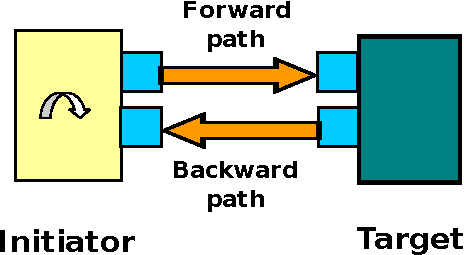
\includegraphics[width=0.6\textwidth]{tlm/figures/nb_fig.pdf}
		\end{center}
		\item Parameters and return value:
		\begin{itemize}
			\item The transaction (\texttt{tlm\_generic\_payload}).
			\item \texttt{\textbf{PHASE}} indicates the state of the transaction: \texttt{\textbf{BEGIN\_REQ}}, \texttt{\textbf{END\_REQ}}, \texttt{\textbf{BEGIN\_RESP}}, and \texttt{\textbf{END\_RESP}}.
			\item The \texttt{sc\_time} parameter indicates the precise simulation time (relative to the last synchronization) the call is taking place.
			\item The return value (\texttt{tlm\_sync\_enum}) indicates the  call status, and fixes synchronization points.
		\end{itemize}
	\end{itemize}
\end{frame}

\begin{frame}
	\frametitle{Non-blocking transport interfaces: Rules (I)}
	\begin{enumerate}
		\item The \texttt{\textbf{nb\_transport\_fw}} and \texttt{\textbf{nb\_transport\_bw}} methods shall not call wait, directly or indirectly.
		\item The \texttt{\textbf{nb\_transport\_fw}} and \texttt{\textbf{nb\_transport\_bw}} methods may be called from a thread process or from a method process.
		\item With the approximately-timed coding style, \texttt{\textbf{nb\_transport\_fw}} and \texttt{\textbf{nb\_transport\_bw}} are called respectively along the forward and backward paths between initiator and target.
		In the case of the generic payload, the two paths should pass through exactly the same sequence of components and sockets, obviously in reverse order.
	\end{enumerate}
\end{frame}

\begin{frame}
	\frametitle{Non-blocking transport interfaces: Rules (II)}
	\begin{enumerate}
		\item The initiator is responsible for deleting or pooling the transaction object after the final timing point. 
		\item If an interconnect component or a target needs to access the state of the transaction after the final call to \texttt{\textbf{nb\_transport\_fw}} or \texttt{\textbf{nb\_transport\_bw}} for a particular transaction instance, it must make a copy of the transaction object.
		\item A \texttt{\textbf{nb\_transport\_fw}} call on the forward path shall under no circumstances directly or indirectly make a call to \texttt{\textbf{nb\_transport\_bw}} on the associated backward path, and vice versa.
	\end{enumerate}
\end{frame}

\begin{frame}
	\frametitle{\small Non-blocking transport interfaces: The \texttt{phase} argument}
	\vspace{0.4em}
	\setbeamercolor{postit}{fg=black,bg=yellow}
	\begin{beamercolorbox}[center,rounded=true,wd=\textwidth]{postit}
		It serves to program protocols phases.
	\end{beamercolorbox}
	\begin{itemize}
		\item<1-> Both caller and callee can modify its value.
		\item The \texttt{tlm\_phase} enum defines four different phase status:
		\begin{itemize}
			\item<1-> \texttt{BEGIN\_REQ}
			\item<1-> \texttt{END\_REQ}
			\item<1-> \texttt{BEGIN\_RESP}
			\item<1-> \texttt{END\_RESP}
		\end{itemize}
	\end{itemize}
	\onslide<2->
	\vspace{-0.9em}
	\begin{center}{
	\scriptsize
	\begin{tabular}{|l|l|l|}
		\hline
		\texttt{\textbf{tlm\_phase}} & \textbf{Coding style} & \textbf{Path} \\
		\hline
		\texttt{BEGIN\_REQ} & Loosely- and approximately-timed & Forward(call) \\
		\hline
		\texttt{END\_REQ} & Approximately-timed only & Forward(return) \\
		& & Backward(call) \\
		\hline
		\texttt{BEGIN\_RESP} & Loosely- and approximately-timed & Forward(return) \\
		& & Backward(call) \\
		\hline
		\texttt{END\_RESP} & Approximately-timed only & Forward(call) \\
		& & Backward(return) \\
		\hline
	\end{tabular}
	}
	\end{center}
\end{frame}

\begin{frame}
	\frametitle{\small Non-blocking transport interface: The \texttt{sc\_time} argument}
	\setbeamercolor{postit}{fg=black,bg=yellow}
	\begin{beamercolorbox}[center,rounded=true,wd=\textwidth]{postit}
		It is used to indicate when the current transaction phase is taking place.
	\end{beamercolorbox}
	\begin{itemize}
		\item<1-> It is always a positive number.
		\item<1-> It is relative to the current simulation time, as returned from \texttt{sc\_time\_stamp}.
	\end{itemize}
	\onslide<2->
	\begin{block}{Temporal decoupling}
		Thanks to this argument the simulators can implement \emph{temporal decoupling}, that is running without yielding control (calling \texttt{wait(\ldots)}) to the SystemC scheduler.
		\newline \newline
		\emph{This enhances the performance of the simulator.}
	\end{block}
\end{frame}

\begin{frame}
	\frametitle{\small Non-blocking transport interface: \texttt{tlm\_sync\_enum} return arg.}
	\setbeamercolor{postit}{fg=black,bg=yellow}
	\begin{beamercolorbox}[center,rounded=true,wd=\textwidth]{postit}
		It signals if the call was a success or something failed, and if a synchronization is needed.
	\end{beamercolorbox}
	Four possible values:
	{\footnotesize
	\definecolor{MyDarkGreen}{rgb}{0,0.45,0}
	\newcommand{\X}{\textbf{\color{MyDarkGreen}$\surd$}}
	\newline
	\begin{tabular}{|l|p{2.5em}|p{2.5em}|l|l|}
		\hline
		\texttt{\textbf{tlm\_sync\_enum}} & \multicolumn{2}{l|}{\textbf{Coding style}} & \textbf{Transaction and} & \textbf{Timing} \\
		\cline{2-3}
		& {\protect \centering LT} & {\protect \centering AT} & \textbf{phase arguments} & \textbf{annotation} \\
		\hline
		\texttt{TLM\_ACCEPTED} & \X & \X & Unmodified &  \\
		\hline
		\texttt{TLM\_UPDATED} & & \X & Updated & \X \\
		\hline
		\texttt{TLM\_COMPLETED} & \X & \X & Updated\tiny{(but caller} & \X \\
		& & & \tiny{may ignore phase)} & \\
		\hline
	\end{tabular}
	}
\end{frame}
}

\mode<article>{
The non-blocking transport interfaces exist to support the loosely-timed and approxitemately-timed coding styles.
Figure~\ref{fig:nb_transport_definition} shows the non-blocking transport interfaces definitions.

\begin{figure}[h]
	\lstinputlisting{tlm/nb_transport.cc}
	\caption{The non-blocking transport interfaces class definitions.}
	\label{fig:nb_transport_definition}
\end{figure}

The non-blocking transport interfaces defines the \texttt{\textbf{nb\_transport\_fw}} and \texttt{\textbf{nb\_transport\_bw}} methods which, as the blocking transport interface method \texttt{\textbf{b\_transport}}, passes a non-const reference to the transaction object.
The \texttt{\textbf{nb\_transport\_fw}} and \texttt{\textbf{nb\_transport\_bw}} methods also passe two other parameters:
\begin{itemize}
	\item a non-const reference to a \texttt{\textbf{PHASE}} object to indicate the state of the transaction, and
	\item a time to annotate the delay of the next phase transition.
\end{itemize}
Additionally the \texttt{\textbf{nb\_transport\_fw}} and \texttt{\textbf{nb\_transport\_bw}} methods can return a value (\texttt{\textbf{tlm\_sync\_enum}}) to indicate the status of the call, and signal synchronization points. 

Unlike the blocking transport interface, the non-blocking transport interfaces needs to be defined by both, the initiator and the target modules.
That is, there is a forward non-blocking transport interface used by the initiator to send requests and a backward non-blocking transport interface used by the target to send the responses.

\subsubsection{Rules}
When using the non-blocking transport interface the following rules must be followed:
\begin{enumerate}
	\item The \texttt{\textbf{nb\_transport\_fw}} and \texttt{\textbf{nb\_transport\_bw}} methods shall not call wait, directly or indirectly.
	\item The \texttt{\textbf{nb\_transport\_fw}} and \texttt{\textbf{nb\_transport\_bw}} methods may be called from a thread process or from a method process.
	\item Exceptionally, if both the blocking and non-blocking transport interfaces are being used together, \texttt{\textbf{nb\_transport\_fw}} may need to call \texttt{\textbf{b\_transport}}. 
	This is only technically possible if it can be guaranteed that the \texttt{\textbf{b\_transport}} method does not call wait, directly or indirectly, but is in any case bad practice.
	Otherwise, the solution is to call to \texttt{\textbf{b\_transport}} from a separate thread process, spawned or notified by the original \texttt{\textbf{nb\_transport\_fw}} call.
	\item With the approximately-timed coding style, \texttt{\textbf{nb\_transport\_fw}} and \texttt{\textbf{nb\_transport\_bw}} mathod are called respectively along the forward and backward paths between initiator and target. 
	In the case of the generic payload, the two paths should pass through exactly the same sequence of components and sockets, obviously in reverse order.
	\item The initiator is responsible for deleting or pooling the transaction object after the final timing point. 
	The final timing point may be marked by a call to or a return from either \texttt{\textbf{nb\_transport\_fw}} on the forward path or \texttt{\textbf{nb\_transport\_bw}} on the backward path. 
	If the final call to non-blocking transport interfaces is on the forward path (i.e. \texttt{\textbf{nb\_transport\_fw}}), the initiator may delete the transaction object on return from \texttt{\textbf{nb\_transport\_fw}}.
	If the final call to non-blocking transport interface is on the backward path (i.e. \texttt{\textbf{nb\_transport\_bw}} , the initiator may delete the transaction object the next time the initiator process resumes, in which case the transaction object shall remain valid and accessible by the target until the target yields to the SystemC scheduler. 
	In other words, if the final call to non-blocking transport interfaces is from target to initiator, the target has a chance to inspect the state of the transaction object before it yields control. 
	After that, any interconnect component or target must assume that the transaction object is invalid.
	\item If an interconnect component or a target needs to access the state of the transaction after the final call to non-blocking transport interfaces for a particular transaction instance, it must make a copy of the transaction object.
	\item A call to non-blocking transport interfaces on the forward path shall under no circumstances directly or indirectly make a call to non-blocking transport interfaces on the associated backward path, and vice versa.
\end{enumerate}

\subsubsection{The \texttt{TRANS} template argument}
The same rules that apply to the transport blocking interface are applied to the non-blocking interface.
However, it must be noted that the life of the transaction expands from the forward request from the initiator starting the request to the backward response from the target module.

\subsubsection{The \texttt{phase} argument}
The phase argument serves to program protocols phases.
The generic payload uses the specific enum \texttt{\textbf{tlm\_phase}}.
Other protocols may substitute it with their own phase types, but this will imply a loss of interoperability.

The \texttt{\textbf{phase}} argument is passed as a non-const reference, which means that both the caller and the callee can change its value.

The \texttt{\textbf{tlm\_phase}} enum defines four different phase status:
\begin{itemize}
	\item \texttt{\textbf{BEGIN\_REQ}}: it marks the beginning of the transaction request.
	It can be used by the approximately-timed coding style.
	The initiator uses this phase when starting a non-blocking transport transaction.
	\item \texttt{\textbf{END\_REQ}}: it marks the end of the transaction request.
	It is only used for the approximately-timed coding style.
	The target uses this phase when finishing a non-blocking transport transaction.
	\item \texttt{\textbf{BEGIN\_RESP}}: it is used by the callee to mark the beginning of the transaction response.
	It can be used by the approximately-timed coding style.
	The transaction callee module can start the response at different points, for example setting the forward call phase argument when returning from a \texttt{\textbf{BEGIN\_REQ}} or \texttt{\textbf{END\_REQ}}, or initiating a backward call.
	\item \texttt{\textbf{END\_RESP}}: it marks the end of the transaction response.
	It is only used for the approximately-timed coding style.
	The initiator uses this phase when finishing a non-blocking transport transaction.
\end{itemize}
Table~\ref{table:tlm_phase_values} summarizes the usage of the \texttt{\textbf{tlm\_phase}} values across the coding styles.
The different values of the phase are used in cycles, but the initiator and target can remove steps if necessary (specially in the case of approximately-timed coding style).
Each time a \texttt{\textbf{BEGIN\_REQ}} is sent a new transaction starts.
Figure~\ref{fig:tlm_phase_sequences} shows the possible phase sequences (note however that these sequences must be used in accordance with the \texttt{tlm\_sync\_enum} return argument).
In section \emph{Loosely-timed coding style} and \emph{Approximately-timed coding style} the different phase values will be explained with examples.

\begin{table}[h]
	\begin{center}
	\begin{tabular}{|l|l|l|}
		\hline
		\texttt{\textbf{tlm\_phase}} & \textbf{Coding style} & \textbf{Path} \\
		\hline
		\texttt{BEGIN\_REQ} & Loosely- and approximately-timed & Forward(call) \\
		\hline
		\texttt{END\_REQ} & Approximately-timed only & Forward(return) Backward(call) \\
		\hline
		\texttt{BEGIN\_RESP} & Loosely- and approximately-timed & Forward(return) Backward(call) \\
		\hline
		\texttt{END\_RESP} & Approximately-timed only & Forward(call) Backward(return) \\
		\hline
	\end{tabular}
	\end{center}
	\caption{Usage of the \texttt{tlm\_phase} values across the coding styles.}
	\label{table:tlm_phase_values}
\end{table}


\begin{figure}[h]
	\begin{center}
\begin{tabular}{|l|}
\hline
\texttt{BEGIN\_REQ} {\footnotesize($\to$ \texttt{BEGIN\_RESP})}\\
\texttt{BEGIN\_REQ} $\to$ \texttt{BEGIN\_RESP}\\
\texttt{BEGIN\_REQ} $\to$ \texttt{END\_REQ} {\footnotesize($\to$ \texttt{BEGIN\_RESP} $\to$ \texttt{END\_RESP})}\\
\texttt{BEGIN\_REQ} $\to$ \texttt{END\_REQ} $\to$ \texttt{BEGIN\_RESP} {\footnotesize($\to$ \texttt{END\_RESP})}\\
\texttt{BEGIN\_REQ} {\small($\to$ \texttt{END\_REQ})} $\to$ \texttt{BEGIN\_RESP} $\to$ \texttt{END\_RESP}\\
\texttt{BEGIN\_REQ} $\to$ \texttt{END\_REQ} $\to$ \texttt{BEGIN\_RESP} $\to$ \texttt{END\_RESP}\\
\hline
\end{tabular}
	\end{center}
	\caption{Permitted phase transition sequences.}
	\label{fig:tlm_phase_sequences}
\end{figure}

\subsubsection{The \texttt{sc\_time} argument}
The \texttt{sc\_time} argument is used to indicate when the current transaction phase is taking place.
It is always a positive number and it is relative to the current simulation time (as the time you can get from \texttt{sc\_time\_stamp()} call). 
So for example if an initiator module calls \texttt{nb\_transport\_fw} it can use the \texttt{sc\_time} argument to indicate the time at which the call is made, without having to do a wait to synchronize itself with the SystemC scheduler.

Thanks to this argument the simulators can implement what is called \emph{temporal decoupling}, that is running without yielding control to the SystemC scheduler.
Avoiding yields to the SystemC scheduler enhances the performance of the simulator.
However it is important to note that it is the responsibility of the simulator writer to handle temporal decoupling.

\subsubsection{The \texttt{tlm\_sync\_enum} return argument}
Once the callee has processed the \texttt{nb\_transport\_fw} or \texttt{nb\_transport\_bw} call it must return the status of the call, signaling if it was a success or something failed, and if a synchronization is needed.
The TLM 2.0 proposes four different status responses:
\begin{itemize}
	\item \texttt{\textbf{TLM\_ACCEPTED}}: The callee accepts the transaction, and the transaction state or time argument should not have been modified during the call.
	The caller should not take further actions on the transaction, and wait for the response from the callee.
	Following the call to \texttt{nb\_transport\_fw} or \texttt{nb\_transport\_bw} the caller should synchronize, this is know as synchronization-on-demand.
	This response is used by the approximately-time coding style.
	\item \texttt{\textbf{TLM\_UPDATED}}: The callee has accepted and updated the transaction, but the transaction has not been completed.
	The callee should have modified the state of the transaction object and the phase argument during the call, and the time argument may have been updated.
	Following the call to \texttt{nb\_transport\_fw} or \texttt{nb\_transport\_bw} the caller should synchronize (synchronization-on-demand).
	This response is used only on approximately-timed coding style.
	\item \texttt{\textbf{TLM\_COMPLETED}}: The transaction has been accepted and completed.
	The caller, after the call to \texttt{nb\_transport\_fw} or \texttt{nb\_transport\_bw} can inspect the contents of the transaction object and the time argument.
	Additionally, the caller can ignore the phase argument because the transaction has been completed.
	There should not be further actions on this transaction once it has been completed.
	This response is used by the approximately-time coding style.
\end{itemize}
Table~\ref{table:tlm_sync_enum_values} summarizes the usage of the \texttt{\textbf{tlm\_phase}} values across the coding styles.

\begin{table}[h]
	\begin{center}
	\begin{tabular}{|l|l|l|l|}
		\hline
		\texttt{\textbf{tlm\_sync\_enum}} & \textbf{Coding style} & \textbf{Transaction and} & \textbf{Timing} \\
		&  & \textbf{phase arguments} & \textbf{annotation} \\
		\hline
		\texttt{TLM\_ACCEPTED} & Loosely- and approximately-timed & Unmodified & No \\
		\hline
		\texttt{TLM\_UPDATED} & Approximately-timed only & Updated & Yes \\
		\hline
		\texttt{TLM\_COMPLETED} & Loosely- and approximately-timed & Updated, but caller & Yes \\
		& & may ignore phase & \\
		\hline
	\end{tabular}
	\end{center}
	\caption{Usage of the \texttt{tlm\_sync\_enum} values across the coding styles.}
	\label{table:tlm_sync_enum_values}
\end{table}

}

\subsection{Direct memory interface}

\mode<presentation>{

\begin{frame}
	\frametitle{DMI: Direct Memory Interface}
	\begin{block}{}
		This interface provides direct access to an area of memory owned by a target.\\
		It bypasses the usual path through the interconnect components used by the transport interface.\\
	\end{block}
	\begin{itemize}
		\item<1-> Intended to {\color{red}accelerate} regular memory transactions in an untimed or loosely-timed simulation.
		\item<1-> DMI is composed by two basic interfaces that must be always be used in conjunction:
		\begin{itemize}
			\item<1-> \texttt{tlm\_fw\_direct\_mem\_if}
			\item<1-> \texttt{tlm\_bw\_direct\_mem\_if}
		\end{itemize}
	\end{itemize}
\end{frame}
}

\mode<article>{
The direct memory interface (DMI) is a specialized interface distinct from the transport interface, providing direct access to an area of memory owned by a target. 
The DMI interface bypass the usual path through the interconnect components used by the transport interface.
DMI is intended to accelerate regular memory transactions in an untimed or loosely-timed simulation.

In this document we will not study this interface in detail.
However you need to know that it exists and its definition because as we will later see it is indirectly used by the classes you will be using when making TLM 2.0 based simulators.

Figure~\ref{fig:tlm_dmi_definition} shows the \texttt{tlm\_dmi} class definition.
DMI is composed of two basic interfaces that must be always be used in conjunction:
\begin{itemize}
	\item \texttt{tlm\_fw\_direct\_mem\_if}: this interface is used by the initiator module to request the target module for a pointer to a memory zone.
	\item \texttt{tlm\_bw\_direct\_mem\_if}: this interface is used by the target module to request the initiator module to invalidate the pointer to a memory zone that was previously provided.
	If the initiator wants to use again the direct access to the memory zone, it must request the memory zone again using the \texttt{tlm\_fw\_direct\_mem\_if}.
\end{itemize}

\begin{figure}[!h]
	\lstinputlisting{tlm/tlm_dmi.hh}
	\caption{The direct memory interfaces class definitions.}
	\label{fig:tlm_dmi_definition}
\end{figure}

In this tutorial we will not be using those interfaces, but we will need to provide an implementation for those interfaces.
The implementation of \texttt{tlm\_fw\_direct\_mem\_if} (done by the target module) should return a \texttt{false}, which indicates to the initiator target that it can not provide a pointer to the memory zone requested.
The implementation of \texttt{tlm\_bw\_direct\_mem\_if} (done by the initiator module) does not need to do anything, because as you will not be requesting the target modules for a pointer to a memory zone, no pointers will need to be invalidated.
However you may add to its implementation an error message to check that your target modules never call this method.
}

\subsection{Debug transaction interface}

\mode<presentation>{

\begin{frame}
	\frametitle{Debug transaction interface}
	\begin{block}{}
		The debug transaction interface provides debug access to an area of memory owned by a target.
	\end{block}
	\begin{itemize}
		\item<1-> It is for debug access free of the delays or side-effects associated with regular transactions.
		\item<1-> It provides a single forward interface:
		\begin{itemize}
			\item<1-> \texttt{tlm\_transport\_dbg\_if}
		\end{itemize}
	\end{itemize}
\end{frame}
}

\mode<article>{
The debug transaction interface is a specialized interface distinct from the transport interface, providing debug access to an area of memory owned by a target. 
The debug transaction interface bypasses the usual path through the interconnect components used by the transport interface. 
The debug transaction interface is for debug access free of the delays or side-effects associated with regular transactions.\footnote{For those of you who know UNISIM-VP, this interface is very close (not to say identical) to the non-intrusive memory interface used by the UNISIM-VP simulators.}

As for the DMI interface, we will not study this interface in detail, however we will briefly present it. 
Figure~\ref{fig:tlm_transport_dbg_if_definition} shows the debug transport interface class definition.
It defines a single forward interface: \texttt{tlm\_transport\_dbg\_if}.
This interface is used by the initiator to access to a memory zone of the target module non-intrusively.

\begin{figure}[!h]
	\lstinputlisting{tlm/tlm_transport_dbg_if.hh}
	\caption{The debug transaction interface class definition.}
	\label{fig:tlm_transport_dbg_if_definition}
\end{figure}

You will need to provide an implementation of this interface on your target modules.
As we will not be using it, you can simply return a \texttt{0} value, which means that your target module can not provide the data requested by the initiator module.
}


\mode<article>{
	\clearpage
}

\section{Sockets and combined interfaces}

\mode<presentation>{
\begin{frame}
	\frametitle{Sockets and combined interfaces}
	A \emph{socket} is a facility class that combines an export with a port.
	Two different sockets:
	\begin{itemize}
		\item<1-> \textbf{initiator}:
		\begin{itemize}
			\item<1-> port for the forward path
			\item<1-> export for the backward path
		\end{itemize}
		\item<1-> \textbf{target}:
		\begin{itemize}
			\item<1-> export for the forward path
			\item<1-> port for the backward path
		\end{itemize}
	\end{itemize}
	\begin{center}
		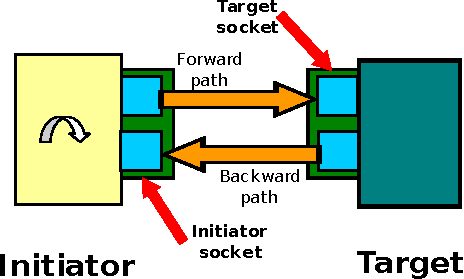
\includegraphics[width=0.6\textwidth]{tlm/figures/socket_fig.pdf}
	\end{center}
\end{frame}

\begin{frame}
	\frametitle{Sockets benefits}
	\begin{itemize}
		\item<1-> They group the transport, direct memory and debug transaction interfaces for both the forward and backward paths together into a single object.
		\item<1-> They provide methods to bind port and export of both the forward and backward paths in a single call.
		\item<1-> They offer strong type checking when binding sockets parameterized with incompatible protocol types.
		\item<1-> They include a bus width parameter that may be used to interpret the transaction.
	\end{itemize}
\end{frame}

\begin{frame}
	\frametitle{Initiator socket definition}
	\lstinputlisting{tlm/tlm_socket_initiator.hh}
\end{frame}

\begin{frame}
	\frametitle{Target socket definition}
	\lstinputlisting{tlm/tlm_socket_target.hh}
\end{frame}

\begin{frame}
	\frametitle{Combined interfaces}
	\lstinputlisting{tlm/combined_interfaces.hh}
\end{frame}

\begin{frame}
	\frametitle{The \texttt{tlm\_generic\_payload\_types}}
	\lstinputlisting{tlm/tlm_socket_types.hh}
\end{frame}
}
\mode<article>{
TLM 2.0 introduced a new facility: the \emph{sockets}.
Sockets are just classes that facilitate the writing of modules using the guidelines proposed by the TLM 2.0 working group.
Two different sockets types are provided: the \emph{initiator} and \emph{target sockets}.
A socket combines a port with and export.
An initiator socket has a port for the forward path and an export for the backward path, whilst a target socket has an export for the forward path and a port for the backward path.
Figures~\ref{fig:tlm_socket_initiator} and ~\ref{fig:tlm_socket_target} show the class definitions for the initiator and the target socket respectively.

\begin{figure}[h]
	\lstinputlisting{tlm/tlm_socket_initiator.hh}
	\caption{The basic initiator socket class definition.}
	\label{fig:tlm_socket_initiator}
\end{figure}

\begin{figure}[h]
	\lstinputlisting{tlm/tlm_socket_target.hh}
	\caption{The basic target socket class definition.}
	\label{fig:tlm_socket_target}
\end{figure}

Sockets use combined interfaces, that is groups of TLM 2.0 interfaces. 
Those combined interfaces include not only transport interfaces, but direct memory and debug transaction interfaces.
Four different combined interfaces exist, combining forward and backward interfaces with blocking and non-blocking transport interfaces.
Figure~\ref{fig:combined_interfaces} shows the class definitions for the four combined interfaces:
\begin{itemize}
	\item blocking transport (identified by the \texttt{\_b\_} infix):
	\begin{itemize}
		\item forward interface (identified by the \texttt{\_fw\_} infix): \texttt{tlm\_fw\_b\_transport\_if}
		\item backware interface (identified by the \texttt{\_bw\_} infix): \texttt{tlm\_bw\_b\_transport\_if}
	\end{itemize}
	\item non-blocking transport (identified by the \texttt{\_nb\_} infix):
	\begin{itemize}
		\item forward interface (identified by the \texttt{\_fw\_} infix): \texttt{tlm\_fw\_nb\_transport\_if}
		\item backware interface (identified by the \texttt{\_bw\_} infix): \texttt{tlm\_bw\_nb\_transport\_if}
	\end{itemize}
\end{itemize}

\begin{figure}[h]
	\lstinputlisting{tlm/combined_interfaces.hh}
	\caption{The four basic combined interfaces class definitions.}
	\label{fig:combined_interfaces}
\end{figure}

The four combined interfaces are parametrized by a single \emph{protocol types class} which defines the different protocols that the interfaces handle.
The default protocol types is the class \texttt{tlm\_generic\_payload\_types} (see Figure~\ref{fig:tlm_socket_types}).
If an application defines a new protocol it should parameterize the combined interfaces with a new protocol types class.

\begin{figure}[h]
	\lstinputlisting{tlm/tlm_socket_types.hh}
	\caption{Basic socket protocol types class.}
	\label{fig:tlm_socket_types}
\end{figure}

Finally, TLM 2.0 includes four convinience classes for inititiator and target socket classes parameterized with the combined interfaces.
Figures~\ref{fig:tlm_socket_blocking} and~\ref{fig:tlm_socket_non_blocking} show the class definitions for the convinience initiator and target socket classes parameterized with the blocking and non-blocking interfaces respectively.
Those classes provide the following benefits:
\begin{itemize}
	\item They group the transport, direct memory and debug transaction interfaces for both the forward and backward paths together into a single object.
	\item They provide methods to bind port and export of both the forward and backward paths in a single call.
	\item They offer strong type checking when binding sockets parameterized with incompatible protocol types.
	\item They include a bus width parameter that may be used to interpret the transaction.
\end{itemize}

\begin{figure}[h]
	\lstinputlisting{tlm/tlm_socket_b.hh}
	\caption{The initiator and target blocking sockets class definitions.}
	\label{fig:tlm_socket_blocking}
\end{figure}

\begin{figure}[h]
	\lstinputlisting{tlm/tlm_socket_nb.hh}
	\caption{The initiator and target non-blocking sockets class definitions.}
	\label{fig:tlm_socket_non_blocking}
\end{figure}

}



\mode<article>{
\clearpage
}

\section{Temporal decoupling and the quantum keeper}

\mode<presentation>{

\begin{frame}
	\frametitle{Temporal decoupling and Quantum Keeper}
	\begin{block}{Temporal decoupling}
		Technique to enhance simulation speed specially adapted for the loosely-timed coding style.\newline
		It allows TLM models to run ahead of the current simulation time without yielding control to the simulation engine (i.e., without calling \texttt{wait(\ldots)}.
	\end{block}
\end{frame}

\begin{frame}
	\frametitle{Temporal decoupling example}
	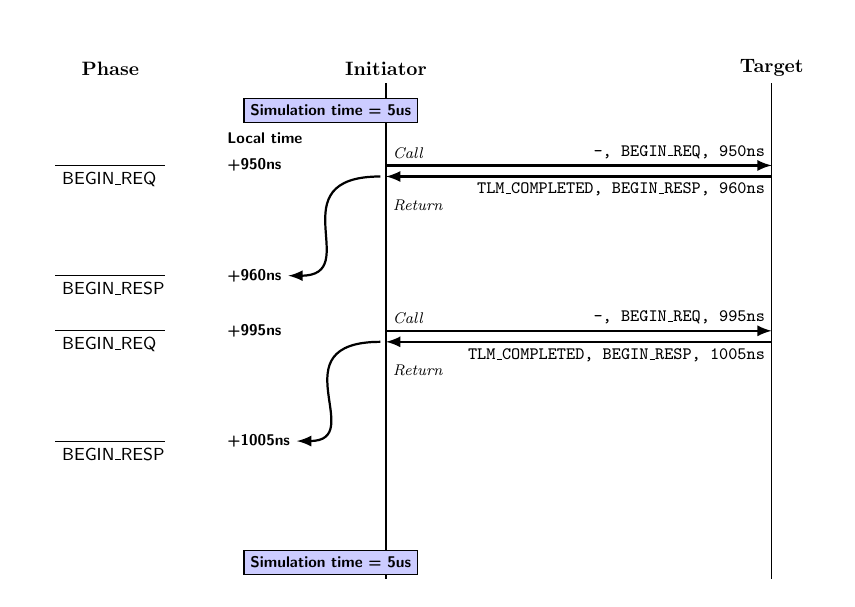
\begin{tikzpicture}[transform shape, scale=0.7]
		\clip (0.5,0) rectangle (15,10);
%		\draw[help lines] (0,0) grid (15,10);
		\path (2,9) coordinate (phase);
		\path (1,7.5) coordinate (req0);
		\path (3,7.5) coordinate (req1);
		\path (1,5.5) coordinate (rsp0);
		\path (3,5.5) coordinate (rsp1);
		\path (1,4.5) coordinate (req1_0);
		\path (3,4.5) coordinate (req1_1);
		\path (1,2.5) coordinate (rsp1_0);
		\path (3,2.5) coordinate (rsp1_1);
		\path (4,8) node(local_time) [right] {\footnotesize \textsf{\textbf{Local time}}};
		\path (4,7.5) node(10ns) [right] {\footnotesize \textsf{\textbf{+950ns}}};
		\path (4,5.5) node(20ns) [right] {\footnotesize \textsf{\textbf{+960ns}}};
		\path (4,4.5) node(35ns) [right] {\footnotesize \textsf{\textbf{+995ns}}};
		\path (4,2.5) node(45ns) [right] {\footnotesize \textsf{\textbf{+1005ns}}};
%		\path (4,1) node(wait) [right] {\footnotesize \textsf{\textbf{wait(1us)}}};
		\path (7,0) coordinate (llb);
		\path (7,9) coordinate (llt);
		\path (14,0) coordinate (rlb);
		\path (14,9) coordinate (rlt);
		\path (7,7.5) coordinate (call_left);
		\path (14,7.5) coordinate (call_right);
		\path (7,7.3) coordinate (ret_left);
		\path (14,7.3) coordinate (ret_right);
		\path (7,4.5) coordinate (call2_left);
		\path (14,4.5) coordinate (call2_right);
		\path (7,4.3) coordinate (ret2_left);
		\path (14,4.3) coordinate (ret2_right);

		\draw (phase) node[above] {\textbf{Phase}};
		\draw (llb) -- (llt)
			node[above] {\textbf{Initiator}};
		\draw (rlb) -- (rlt)
			node[above] {\textbf{Target}};
		\draw (req0) node[below right] {\small \textsf{BEGIN\_REQ}} -- (req1);
		\draw (rsp0) node[below right] {\small \textsf{BEGIN\_RESP}} -- (rsp1);
		\draw (req1_0) node[below right] {\small \textsf{BEGIN\_REQ}} -- (req1_1);
		\draw (rsp1_0) node[below right] {\small \textsf{BEGIN\_RESP}} -- (rsp1_1);
		\draw[thick,-latex] (call_left) -- (call_right);
		\draw (call_left) node[above right] {\footnotesize \emph{Call}};
		\draw (call_right) node[above left] {\small \texttt{\textbf{-, BEGIN\_REQ, 950ns}}};
		\draw[thick,latex-] (ret_left) -- (ret_right);
		\draw (ret_left) +(0,-0.3) node[below right] {\footnotesize \emph{Return}};
		\draw (ret_right) node[below left] {\small \texttt{\textbf{TLM\_COMPLETED, BEGIN\_RESP, 960ns}}};
		\draw[thick,-latex] (call2_left) -- (call2_right);
		\draw (call2_left) node[above right] {\footnotesize \emph{Call}};
		\draw (call2_right) node[above left] {\small \texttt{\textbf{-, BEGIN\_REQ, 995ns}}};
		\draw[thick,latex-] (ret2_left) -- (ret2_right);
		\draw (ret2_left) +(0,-0.3) node[below right] {\footnotesize \emph{Return}};
		\draw (ret2_right) node[below left] {\small \texttt{\textbf{TLM\_COMPLETED, BEGIN\_RESP, 1005ns}}};
		\path (6,8.5) node(100ns) [rectangle,draw,fill=blue!20] {\footnotesize \textsf{\textbf{Simulation time = 5us}}};
		\path (6,0.3) node(110ns) [rectangle,draw,fill=blue!20] {\footnotesize \textsf{\textbf{Simulation time = 5us}}};
		\path (ret_left) +(-2,0) coordinate (control_ret_left);
		\path (20ns) +(2,0) coordinate (control_20ns);
		\draw[thick,-latex] (ret_left) +(-0.1,0) .. controls (control_ret_left) and (control_20ns) .. (20ns)[above];
		\path (ret2_left) +(-2,0) coordinate (control_ret2_left);
		\path (45ns) +(2,0) coordinate (control_45ns);
		\draw[thick,-latex] (ret2_left) +(-0.1,0) .. controls (control_ret2_left) and (control_45ns) .. (45ns)[above];
	\end{tikzpicture}
\end{frame}

\begin{frame}
	\frametitle{Temporal decoupling and Quantum Keeper}
	\begin{block}{Temporal decoupling}
		Technique to enhance simulation speed specially adapted for the loosely-timed coding style.\newline
		It allows TLM models to run ahead of the current simulation time without yielding control to the simulation engine (i.e., without calling \texttt{wait(\ldots)}.
	\end{block}
	\alert{Beware of process inanition.}
	\begin{itemize}
		\item<2-> Solution:
		\begin{itemize}
			\item<2-> The Quantum Keeper
		\end{itemize}
	\end{itemize}
\end{frame}

\begin{frame}
	\frametitle{The Quantum Keeper (\texttt{tlm\_quantum\_keeper})}
	\begin{itemize}
		\item Convenience class to control avoid inanition.
	\end{itemize}
	\lstinputlisting{tlm/quantum_keeper.hh}
\end{frame}

\begin{frame}
	\frametitle{Quantum Keeper example}
	\lstinputlisting[linerange={1-13, 34-35}]{tlm/quantum_keeper_example.hh}
\end{frame}

\begin{frame}
	\frametitle{Quantum Keeper example (cont.)}
	\lstinputlisting[linerange={1-2, 14-35}]{tlm/quantum_keeper_example.hh}
\end{frame}
}

\mode<article>{
\emph{Temporal decoupling} is a powerful technique to enhance SystemC simulation speed specially adapted for the loosely-timed coding style.
Basically it consist on doing as much work as possible inside a module process without yielding the control to the SystemC simulation engine\footnote{That is, without performing any call to \texttt{wait(\ldots)}.}.
So this technique allows TLM models to run ahead of the current simulation time (as it is returned by \texttt{sc\_time\_stamp()}).

\begin{figure}[h]
	\begin{center}
	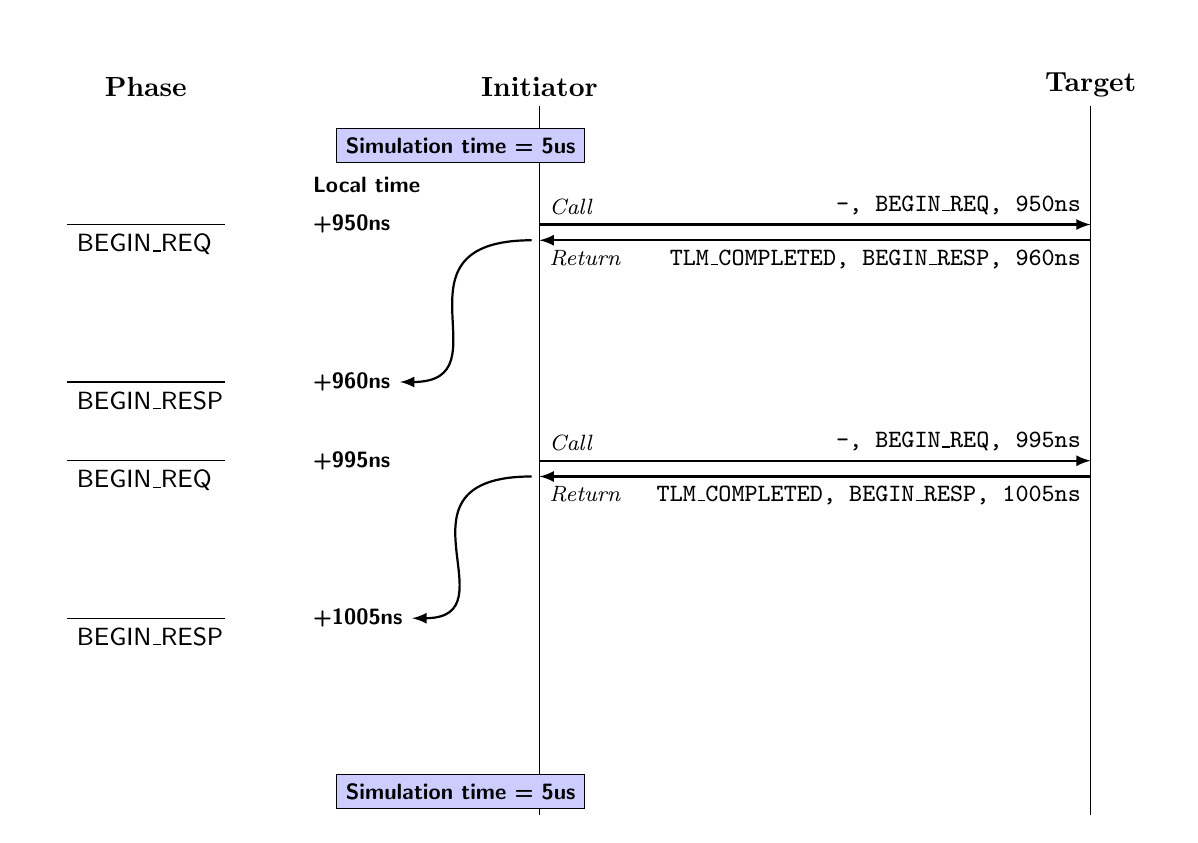
\begin{tikzpicture}
		\clip (0.5,0) rectangle (15,10);
%		\draw[help lines] (0,0) grid (15,10);
		\path (2,9) coordinate (phase);
		\path (1,7.5) coordinate (req0);
		\path (3,7.5) coordinate (req1);
		\path (1,5.5) coordinate (rsp0);
		\path (3,5.5) coordinate (rsp1);
		\path (1,4.5) coordinate (req1_0);
		\path (3,4.5) coordinate (req1_1);
		\path (1,2.5) coordinate (rsp1_0);
		\path (3,2.5) coordinate (rsp1_1);
		\path (4,8) node(local_time) [right] {\footnotesize \textsf{\textbf{Local time}}};
		\path (4,7.5) node(10ns) [right] {\footnotesize \textsf{\textbf{+950ns}}};
		\path (4,5.5) node(20ns) [right] {\footnotesize \textsf{\textbf{+960ns}}};
		\path (4,4.5) node(35ns) [right] {\footnotesize \textsf{\textbf{+995ns}}};
		\path (4,2.5) node(45ns) [right] {\footnotesize \textsf{\textbf{+1005ns}}};
%		\path (4,1) node(wait) [right] {\footnotesize \textsf{\textbf{wait(1us)}}};
		\path (7,0) coordinate (llb);
		\path (7,9) coordinate (llt);
		\path (14,0) coordinate (rlb);
		\path (14,9) coordinate (rlt);
		\path (7,7.5) coordinate (call_left);
		\path (14,7.5) coordinate (call_right);
		\path (7,7.3) coordinate (ret_left);
		\path (14,7.3) coordinate (ret_right);
		\path (7,4.5) coordinate (call2_left);
		\path (14,4.5) coordinate (call2_right);
		\path (7,4.3) coordinate (ret2_left);
		\path (14,4.3) coordinate (ret2_right);

		\draw (phase) node[above] {\textbf{Phase}};
		\draw (llb) -- (llt)
			node[above] {\textbf{Initiator}};
		\draw (rlb) -- (rlt)
			node[above] {\textbf{Target}};
		\draw (req0) node[below right] {\small \textsf{BEGIN\_REQ}} -- (req1);
		\draw (rsp0) node[below right] {\small \textsf{BEGIN\_RESP}} -- (rsp1);
		\draw (req1_0) node[below right] {\small \textsf{BEGIN\_REQ}} -- (req1_1);
		\draw (rsp1_0) node[below right] {\small \textsf{BEGIN\_RESP}} -- (rsp1_1);
		\draw[thick,-latex] (call_left) -- (call_right);
		\draw (call_left) node[above right] {\footnotesize \emph{Call}};
		\draw (call_right) node[above left] {\small \texttt{\textbf{-, BEGIN\_REQ, 950ns}}};
		\draw[thick,latex-] (ret_left) -- (ret_right);
		\draw (ret_left) node[below right] {\footnotesize \emph{Return}};
		\draw (ret_right) node[below left] {\small \texttt{\textbf{TLM\_COMPLETED, BEGIN\_RESP, 960ns}}};
		\draw[thick,-latex] (call2_left) -- (call2_right);
		\draw (call2_left) node[above right] {\footnotesize \emph{Call}};
		\draw (call2_right) node[above left] {\small \texttt{\textbf{-, BEGIN\_REQ, 995ns}}};
		\draw[thick,latex-] (ret2_left) -- (ret2_right);
		\draw (ret2_left) node[below right] {\footnotesize \emph{Return}};
		\draw (ret2_right) node[below left] {\small \texttt{\textbf{TLM\_COMPLETED, BEGIN\_RESP, 1005ns}}};
		\path (6,8.5) node(100ns) [rectangle,draw,fill=blue!20] {\footnotesize \textsf{\textbf{Simulation time = 5us}}};
		\path (6,0.3) node(110ns) [rectangle,draw,fill=blue!20] {\footnotesize \textsf{\textbf{Simulation time = 5us}}};
		\path (ret_left) +(-2,0) coordinate (control_ret_left);
		\path (20ns) +(2,0) coordinate (control_20ns);
		\draw[thick,-latex] (ret_left) +(-0.1,0) .. controls (control_ret_left) and (control_20ns) .. (20ns)[above];
		\path (ret2_left) +(-2,0) coordinate (control_ret2_left);
		\path (45ns) +(2,0) coordinate (control_45ns);
		\draw[thick,-latex] (ret2_left) +(-0.1,0) .. controls (control_ret2_left) and (control_45ns) .. (45ns)[above];
	\end{tikzpicture}
	\end{center}
	\caption{Loosely-timed coding style with temporal decoupling example.}
	\label{fig:temporal_decoupling_example}
\end{figure}

Figure~\ref{fig:temporal_decoupling_example} shows an example of a loosely-timed coding style model using temporal decoupling.
However, this technique can be dangerous, producing inanition of other processes which are waiting for SystemC to execute them.
Simply imagine that the initiator in Figure~\ref{fig:temporal_decoupling_example} never performs a \texttt{wait(\ldots)} and other initiator processes in the system never get execution.
So, when using the temporal decoupling technique care must be taken to avoid inanition.

\begin{figure}[h]
	\lstinputlisting{tlm/quantum_keeper.hh}
	\caption{The quantum keeper class definition.}
	\label{fig:quantum_keeper_definition}
\end{figure}

To facilitate the task of avoiding inanition, TLM 2.0 provides the convenience class \texttt{tlm\_quantum\_keeper} (aka. The Quantum Keeper).
It provides a set of methods for managing and interacting with the time quantum. 
It is recommended to use it in order to maintain a consistent coding style (but not compulsory).
Figure~\ref{fig:quantum_keeper_definition} shows the class definition of the quantum keeper.

\begin{figure}[h]
	\lstinputlisting{tlm/quantum_keeper_example.hh}
	\caption{Example of a loosely-timed initiator using the quantum keeper.}
	\label{fig:quantum_keeper_example}
\end{figure}

Basically this class keeps track of the module local time and synchronizes when necessary with the SystemC simulation time when necessary.
The user must define the time threshold the modules can run ahead of time using the static method \texttt{set\_global\_quantum}.
When the module local time difference with the simulation time reaches the user defined threshold the quantum keeper notifies the module that it must synchronize, that is, that is must perform a \texttt{wait(\ldots)} with the amount of time signaled by the quantum keeper.
Figure~\ref{fig:quantum_keeper_example} shows the example of a loosely-timed initiator using the quantum keeper.

Note that the user must define the time threshold for the quantum keeper globally, so no module should ever call the \texttt{set\_global\_quantum}.
Usually the quantum keeper time threshold is set up globally before or after the assembly of the simulator modules and before calling \texttt{sc\_start}.
To have a global quantum keeper time threshold helps to avoid inanition, because all the modules will share the same threshold.
The threshold is also a toggle between simulation speed and simulation accuracy, the bigger its value the less modules will yield and the faster the simulation will be. 
The smaller its value the more modules will yield and the slower the simulation will be.
}


\mode<article> {
	\clearpage
}

\section{The Generic Payload}

\mode<presentation>{

\begin{frame}
	\frametitle{The generic payload}
	\begin{block}{Objective}
		Improve interoperability between modules providing a single message type for most TLM designs.
	\end{block}
	\begin{itemize}
		\item \texttt{tlm\_generic\_payload} provides a generic message type.
		\item It is specifically aimed at memory mapped buses.
		\item It provides an extension mechanism to add ignorable extension.
		\item It can be used to generate new payload types.
	\end{itemize}
\end{frame}

\begin{frame}
	\frametitle{\texttt{tlm\_generic\_payload} class definition}
	\lstinputlisting[linerange={1-31}]{tlm/tlm_generic_payload.hh}
\end{frame}

\begin{frame}
	\frametitle{\small \texttt{tlm\_generic\_payload} class definition (contd.)}
	\lstinputlisting[linerange={31-53}]{tlm/tlm_generic_payload.hh}
\end{frame}
}

\mode<article>{
Unlike TLM 1.0, TLM 2.0 introduced a generic message type (payload).
With a generic payload, the SystemC TLM working group expects to improve the interoperability of modules written with SystemC TLM.
Effectively, one of the drawbacks of TLM 1.0 was that the payload was not standardized.
This made difficult the connection of modules that should have been easy to connect.
For example a simple address type could make two modules speaking the same protocol not interoperable.

The generic payload is specifically aimed at memory-mapped buses. 
This guarantees the interoperability of abstract models using memory-mapped buses for which precise details are unimportant.
Additionally it provides an extension mechanism which allow the designer to add details which may be \emph{ignorable}, thus not breaking the interoperability of the models, but enhancing their functionality if the connected models implement such ignorable details.

The same extension mechanism allows the designer to add bus specific details which maybe compulsory.
If such is the case, the connected models using the specific bus will need to implement such extension.
It is the responsibility of the provider of the extension to provide models which use it, models which bridge with the generic payload, or to provide coding guidelines for the usage of such extension.

The use of ignorable extensions allow the connection of two models with different payloads:
\begin{itemize}
	\item One of the models could use the generic payload without extensions and the other the generic payload with ignorable extensions.
	\item The two models could use different ignorable extensions over the generic payload.
\end{itemize}
Any of those combinations would compile, and produce an executable simulator.

However, the TLM working group recommends a disciplined use of the ignorable extensions.
Effectively, the designers could use the ignorable extensions to allow full compilation interoperability, but those models would check the non ignorable extensions at run-time, what would degrade the simulation performance or simply create simulators that would dump an error message systematically.
For that reason, there are three, \emph{an only three}\footnote{The TLM working group heavily insist on that point.} recommended alternatives for the transaction template argument of blocking and non-blocking interfaces (ordered from more interoperability to less interoperability solutions):
\begin{enumerate}
	\item \emph{Use the generic payload, with ignorable extensions.}\newline
	In this case the ignorable extensions should be clearly ignorable, that is, the models should not create an error message or fail if the extension is not available.
	Neither the model should work in degraded mode.
	Examples of correct ignorable extensions are:
	\begin{itemize}
		\item There is a clear default value for the ignorable extension.
		\item The extension contains simulation-related information, but not model behavior related information.
	\end{itemize}
	\item \emph{Define a new protocol types class containing a \texttt{typedef} for \texttt{tlm\_generic\_payload}.}\newline
	When the extensions are clearly not ignorable, but the new protocol is a clear extension of the \texttt{tlm\_generic\_payload}, this solution is recommended.
	This allows a rapid development of the new payload type thanks to the reuse the generic payload, but at the same time this ensures that compile time interoperability checking of two interconnected models.
	\item \emph{Define a new protocol types class and a new transaction type.}\newline
	When the generic payload is clearly ill adapted to create the transaction and protocol a new protocol types class and a new transaction type should be defined.
	Again, this ensures the compile time interoperability checking of two connected models.
\end{enumerate}

%\begin{figure}[h]
%	\lstinputlisting{tlm/tlm_generic_payload_types.hh}
%	\caption{The types used by the generic payload class definitions.}
%	\label{fig:tlm_generic_payload_types}
%\end{figure}

\begin{figure}[h]
	\lstinputlisting{tlm/tlm_generic_payload.hh}
	\caption{The generic payload class definition.}
	\label{fig:tlm_generic_payload_definition}
\end{figure}

Figure~\ref{fig:tlm_generic_payload_definition} shows the definition of the \texttt{tlm\_generic\_payload} class.
The initiator of a transaction is responsible of the creation of all the storage that the generic payload may require during its lifetime. 
Additionally, it is responsible of keeping the generic payload available during the lifetime of the transaction.

\begin{table}[h]
	\begin{center}
	\begin{tabular}{|l|l|l|l|}
	\hline
	\textbf{Attribute} & \textbf{Default value} & \textbf{Modifiable by} & \textbf{Modifiable by} \\
	& & \textbf{interconnect?} & \textbf{target?} \\
	\hline
	Command & \texttt{TLM\_IGNORE\_COMMAND} & No & No \\
	\hline
	Address & 0 & Yes & No \\
	\hline
	Data pointer & 0 & No & No \\
	\hline
	Data array & - & No & Yes (read) \\
	\hline
	Data length & 1 & No & No \\
	\hline
	Byte enable pointer & 0 & No & No \\
	\hline
	Byte enable array & - & No & No \\
	\hline
	Byte enable length & 1 & No & No \\
	\hline
	Streaming width & 0 & No & No \\
	\hline
	DMI allowed & false & Yes & Yes \\
	\hline
	Response status & \texttt{TLM\_INCOMPLETE\_RESPONSE} & No & Yes \\
	\hline
	Extension pointers & 0 & Yes & Yes \\
	\hline
	\end{tabular}
	\end{center}
	\caption{Generic payload default values and modifiability of attributes}
	\label{table:tlm_generic_payload_default_values}
\end{table}

When created the values of the different generic payload attributes shall be set as defined in Table~\ref{table:tlm_generic_payload_default_values}.
The copy constructor should make a shallow copy of the payload contents, that is the different pointer should be copied but not their contents.
The same applies for the assignment operator.
The \texttt{deep\_copy} method on the other side should additionally copy the contents of the pointers. Implementations of the virtual destructor should not delete the data array, the byte enable array, or any extension objects.

The generic payload attributes are not publicly accessible and should be set and get using the provided setters and getters. 
Table~\ref{table:tlm_generic_payload_default_values} shows which attributes can be modified by interconnect and target modules.
}

\subsection{The command attribute}

\mode<presentation>{

\begin{frame}
	\frametitle{The command attribute}
	\begin{itemize}
		\small
		\item<1-> Only three commands are defined:
		\lstinputlisting{tlm/tlm_command.hh}
		\item<2-> Getter and setter:
		\begin{itemize}
			\item<2-> \texttt{tlm\_command get\_command()}
			\item<2-> \texttt{void set\_command(const tlm\_command)}
		\end{itemize}
		\item<2-> Facility methods are provided to set a read/write request, and to check: \texttt{is\_read()}, \texttt{set\_read()}, \texttt{is\_write()} and \texttt{set\_write()}.
		\item<3-> Default error when command not supported: \texttt{TLM\_COMMAND\_ERROR\_RESPONSE}
		\item<4-> When the command is \texttt{TLM\_IGNORE\_COMMAND}, the target must ignore data pointer, but can use any other attributes, including extensions.
	\end{itemize}
\end{frame}

}

\mode<article>{
\begin{figure}[h]
	\lstinputlisting{tlm/tlm_command.hh}
	\caption{Definition of the different generic payload commands.}
	\label{fig:tlm_command}
\end{figure}

Figure~\ref{fig:tlm_command} shows the different commands provided by the command attribute.
Only read, write and ignore commands are provided.
The generic payload provides a setter and getter to set and get the command, and convenience methods to set and get them: \texttt{is\_read()}, \texttt{is\_write()}, \texttt{set\_read()}, \texttt{set\_write()}.

When receiving a read command the target should fill the array pointed by the data pointer attribute.
When receiving a write command the target should copy the array pointed by the data pointer attribute.
If the target is unable to execute a read or write command, it shall generate a standard error response (\texttt{TLM\_COMMAND\_ERROR\_RESPONSE} is recommended).
When receiving an ignore command the target should ignore the contents of the data pointer, but can use any other attribute in the payload, including extensions.
}

\subsection{The address attribute}

\mode<presentation>{

\begin{frame}
	\frametitle{The address attribute}
	\begin{itemize}
		\item<1-> It corresponds to the first byte in the array pointed by the data pointer attribute.
		\item<1-> Getter and setter:
		\begin{itemize}
			\item<1-> \texttt{sc\_dt::uint64 get\_address()}
			\item<1-> \texttt{void set\_address(const sc\_dt::uint64)}
		\end{itemize}
		\item<2-> Formula: \textbf{$address\_attribute + (array\_index \% streaming\_width)$}
		\item<3-> Default error when error in address: \texttt{TLM\_ADDRESS\_ERROR\_RESPONSE}
		\item<3-> Interconnect modules may change its value (for example when a translation needs to be made).
	\end{itemize}
\end{frame}
}

\mode<article>{
The address received by the target should be considered as the first byte to be read from or written to the local array in the target.
It always corresponds to the first byte in the array pointed by the data pointer attribute.

A byte at a given index in the data array shall be transferred to or from the address given by the formula \textbf{$address\_attribute + (array\_index \% streaming\_width)$}.

If the requested command can not be performed in the given address (or address range) an standard error should be returned (\texttt{TLM\_ADDRESS\_ERROR\_RESPONSE} is recommended).

The address attribute is set by the initiator module. Target module should not modify it, however, interconnect modules can modify its value.
It could be the case if the interconnect module needs to do some kind of address translation on the transaction.
}

\subsection{The data pointer attribute}

\mode<presentation>{

\begin{frame}
	\frametitle{The data pointer attribute}
	\begin{itemize}
		\item<1-> Buffer allocated by the initiator module to perform the read/write command.
		\item<1-> Getter and setter:
		\begin{itemize}
			\item<1-> \texttt{unsigned char* get\_data\_ptr()}
			\item<1-> \texttt{void set\_data\_ptr(unsigned char *)}
		\end{itemize}
		\item<2-> Must be always different than 0 (\texttt{NULL}).
		\item<2-> Should never be modified by interconnect modules.
		\item<2-> The size of the buffer must be bigger than the number of bytes to read/write (the data lengt attribute).
	\end{itemize}
\end{frame}

}

\mode<article>{
The data pointer attribute should point to a buffer allocated by the initiator module.
The data pointer should always be set to something different than 0 before calling the transport interface.
Such buffer should contain the data to be written into the target on write command, and a buffer to write the data to be read from the target on read command.
Interconnect modules should never modify the contents of the buffer.
The size of the buffer should always be bigger than the number of bytes to read/write (the data length attribute).
}

\subsection{The data length attribute}

\mode<presentation>{

\begin{frame}
	\frametitle{The data length attribute}
	\begin{itemize}
		\item<1-> It represents the length in bytes to be read/written, inclusive for any bytes disabled by the byte enable attribute.
		\item<1-> Getter and setter:
		\begin{itemize}
			\item<1-> \texttt{unsigned int get\_data\_length()}
			\item<1-> \texttt{void set\_data\_length(const unsigned int)}
		\end{itemize}
		\item<2-> If it is bigger than the template parameter BUSWIDTH, the transfer is considered as a burst transfer.
		\item<2-> Default error when error due to the data length attribute: \texttt{TLM\_BURST\_ERROR\_RESPONSE}.
	\end{itemize}
\end{frame}

}

\mode<article>{
It represents the length in bytes to be read/written, inclusive for any bytes disabled by the byte enable attribute.
This attribute shall be set by the initiator module, and not modified by any interconnect or target module.

If the data length is bigger than the template parameter \texttt{BUSWIDTH} (in bits) the transfer is considered as a burst transfer.
The size of the transfer on those cases is the \texttt{BUSWIDTH}.
If the data length is smaller than or equal to \texttt{BUSWIDTH} the transfer is a word transfer, not a burst transfer.

If the target can not satisfy the request given the received data length, it should generate a standard error response (\texttt{TLM\_BURST\_ERROR\_RESPONSE} is recommended).
}

\subsection{The byte enable pointer and the byte enable length attributes}

\mode<presentation>{

\begin{frame}
	\frametitle{The byte enable pointer and length attributes}
	\begin{itemize}
		\item<1-> Define the bytes that should be read from or written to the data buffer.
		\item<1-> The byte enable length defines the size of the byte enable array.
		\item<1-> Getter and setter:
		\begin{itemize}
			\item<1-> \texttt{unsigned char* get\_byte\_enable\_ptr()}
			\item<1-> \texttt{void set\_byte\_enable\_ptr(unsigned char *)}
			\item<1-> \texttt{unsigned int get\_byte\_enable\_length()}
			\item<1-> \texttt{void set\_byte\_enable\_length(const unsigned int)}
		\end{itemize}
		\item<2-> Formula: $byte\_enable\_array\_index = data\_array\_index \% byte\_enable\_length$
		\item<2-> If length is equal to 0, the byte enable array can be ignored.
		\item<3-> Default error response because byte enable error: \texttt{TLM\_BYTE\_ENABLE\_ERROR\_RESPONSE}
	\end{itemize}
\end{frame}
}

\mode<article>{
Those couple of attributes define the bytes that should be read from or written to the data buffer.
The byte enable length attribute defines the size of the byte enable pointer.
The byte enable pointer attribute points to an array of booleans that defines the mask of bytes that should be considered(true value)/ignored(false value).

If the byte enable length attribute is smaller than the data length attribute, the contents of the byte enable pointer should be considered as many times as necessary to match the data length attribute.
The following formula can be used $byte\_enable\_array\_index = data\_array\_index \% byte\_enable\_length$.

If the byte enabled pointer is equal to 0 the byte enable length attribute must be ignored, and bytes enables should be also ignored (all the contents of the data array should be considered).

If the target can not process the requested transaction because of the byte enable pointer or the byte enable length attributes, a standard error should be returned (TLM\_BYTE\_ENABLE\_ERROR\_RESPONSE is recommended).
}

\subsection{The streaming width attribute}

\mode<presentation>{

\begin{frame}
	\frametitle{The streaming width attribute}
	\begin{itemize}
		\item<1-> It determines the width of the stream, that is, the number of bytes transferred on each beat.
		\item<1-> Getter and setter:
		\begin{itemize}
			\item<1-> \texttt{unsigned int get\_streaming\_width()}
			\item<1-> \texttt{void set\_streaming\_width(unsigned int)}
		\end{itemize}
		\item<2-> Formula: \textbf{$address\_attribute + (array\_index \% streaming\_width)$}
		\item<2-> If its value is equal to 0, then the transfer is considered as a normal transfer (or burst transfer).
		\item<3-> Default error on stream width error: \texttt{TLM\_BURST\_ERROR\_RESPONSE}.
	\end{itemize}
\end{frame}

}

\mode<article>{
Streaming affects the way a component should interpret the data array. 
A stream consists of a sequence of data transfers occurring on successive notional beats. 
The streaming width attribute shall determine the width of the stream, that is, the number of bytes transferred on each beat.

The address to or from which each byte is being copied in the target shall be reset to the value of the address attribute at the start of each beat.

With respect to the interpretation of the data array, a transaction with a non-zero streaming width shall be functionally equivalent to a sequence of transactions each having the same address as the original transaction, each having a data length attribute equal to the streaming width of the original, and each with a data array that effectively steps down the original data array maintaining the sequence of bytes.

A streaming width of 0 shall be interpreted in the same way as a streaming width greater than or equal to the value of the data length attribute, that is, the data transfer is a normal transfer, not a streaming transfer.

If the target module can not process the transfer because of the streaming width attribute a standard error should be returned (\texttt{TLM\_BURST\_ERROR\_RESPONSE} is recommended).
}

\subsection{Endianess}

\mode<presentation>{

\begin{frame}
	\frametitle{Endianess}
	\begin{block}{}
		In order to interpret the contents of the data pointer array TLM 2.0 defines that the data transferred should be sent using the host endianness.
	\end{block}
\end{frame}

}

\mode<article>{
In order to interpret the contents of the data pointer array TLM 2.0 defines that the data transferred should be sent using the host endianness.
}

\subsection{DMI allowed attribute}

\mode<presentation>{

\begin{frame}
	\frametitle{DMI allowed attribute}
	\begin{itemize}
		\item<1-> Thanks to this attribute the target module can give a hint to the initiator module signaling if the target supports or not DMI for the current request.
		\item<1-> Getter and setter:
		\begin{itemize}
			\item<1-> \texttt{void set\_dmi\_allowed(bool)}
			\item<1-> \texttt{bool get\_dmi\_allowed()}
		\end{itemize}
	\end{itemize}
\end{frame}
}

\mode<article>{
Thanks to this attribute the target module can give a hint to the initiator module signaling if the target supports or not DMI for the current request.
}

\subsection{The response status attribute}

\mode<presentation>{

\begin{frame}
	\frametitle{The response status attribute}
	\begin{itemize}
		\item<1-> Possible error attribute values:
		\lstinputlisting{tlm/tlm_response_status.hh}
		\item<1-> Getter and setter:
		\begin{itemize}
			\item<1-> \texttt{tlm\_response\_status get\_response\_status()}
			\item<1-> \texttt{void set\_response\_status(const tlm\_response\_status)}
		\end{itemize}
		\item<2-> Helper methods:
		\begin{itemize}
			\item<2-> \texttt{std::string get\_response\_string()}
			\item<2-> \texttt{bool is\_response\_ok()}
			\item<2-> \texttt{bool is\_response\_error()}
		\end{itemize}
	\end{itemize}
\end{frame}
}

\mode<article>{
\begin{figure}[h]
	\lstinputlisting{tlm/tlm_response_status.hh}
	\caption{Definition of the different response status values.}
	\label{fig:tlm_response_status_definition}
\end{figure}

\begin{table}[h]
	\begin{center}
	\begin{tabular}{|l|l|}
		\hline
		\textbf{Error response} & \textbf{Interpretation} \\
		\hline
		\texttt{TLM\_ADDRESS\_ERROR\_RESPONSE} & Unable to act upon the address attribute, \\
		& or address out of range\\
		\hline
		\texttt{TLM\_COMMAND\_ERROR\_RESPONSE} & Unable to execute the command \\
		\hline
		\texttt{TLM\_BURST\_ERROR\_RESPONSE} & Unable to act upon the data length or streaming width \\
		\hline
		\texttt{TLM\_BYTE\_ENABLE\_ERROR\_RESPONSE} & Unable to act upon the byte enable \\
		\hline
		\texttt{TLM\_GENERIC\_ERROR\_RESPONSE} & Any other error	\\
		\hline
	\end{tabular}
	\end{center}
	\caption{Error response values}
	\label{table:response_status_errors}
\end{table}

Figure~\ref{fig:tlm_response_status_definition} shows the response status attribute possible values.
This attribute is used by the target module to signal the success (\texttt{TLM\_OK\_RESPONSE}) if the transaction could successfully handled, and to an error otherwise, following the Table~\ref{table:response_status_errors}.
The initiator should set this attribute to \texttt{TLM\_INCOMPLETE\_RESPONSE}, and no interconnect module should modify it, because it means that the target module has not still handled the transaction.
}

\subsection{The extension mechanism}

\mode<article>{
The extension mechanism is out of the scope of this tutorial.
For a detailed explanation refer to the Accellera TLM 2.0 User Manual.
}


\mode<article>{
	\clearpage
}

\section{Message charts examples}

\mode<presentation>{

\begin{frame}
	\frametitle{Message charts examples}
	\begin{itemize}
		\item<1-> Untimed
		\item<1-> Loosely-timed with timing annotation
		\item<1-> Loosely-timed with sync
		\item<1-> Loosely-timed with temporal decoupling
		\item<1-> Loosely-timed with temporal decoupling and synchronization-on-demand
		\item<1-> Loosely-timed with temporal decoupling and quantum
		\item<1-> Approximately-timed using backward path
		\item<1-> Approximately-timed with timing annotation
		\item<1-> Approximately-timed with polling
	\end{itemize}
\end{frame}

}

\mode<article>{
In the following subsections you will find charts explaining the message exchanges examples when using the different coding styles.
}

\subsection{Untimed}

\mode<presentation>{
\begin{frame}
	\frametitle{Untimed}

\begin{figure}[h]
	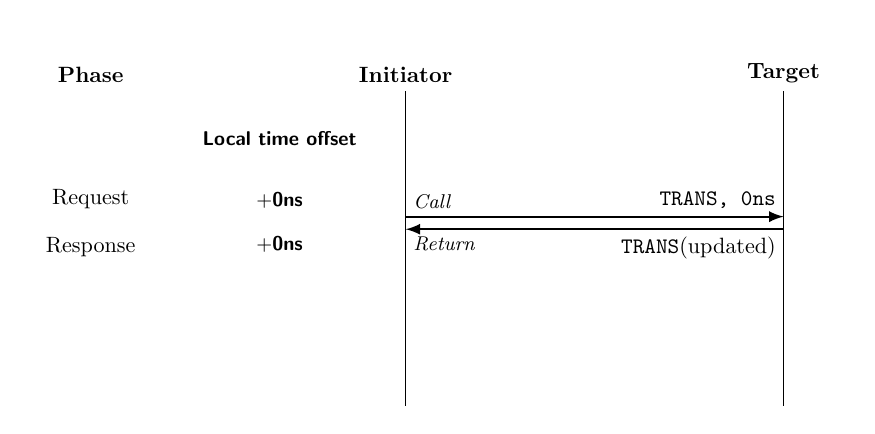
\begin{tikzpicture}[transform shape,scale=0.8]
		\clip (1,0) rectangle (14,6);
%		\draw[help lines] (0,0) grid (15,10);
		\path (2,5) coordinate (phase);
		\path (2,3) coordinate (req);
		\path (2,2.8) coordinate (rsp);
		\path (5,4) coordinate (time);
		\path (5,3) coordinate (0ns);
		\path (5,2.8) coordinate (0nstext);
		\path (7,0) coordinate (llb);
		\path (7,5) coordinate (llt);
		\path (13,0) coordinate (rlb);
		\path (13,5) coordinate (rlt);
		\path (7,3) coordinate (call_left);
		\path (13,3) coordinate (call_right);
		\path (7,2.8) coordinate (ret_left);
		\path (13,2.8) coordinate (ret_right);

		\onslide*<1-> {
		\draw (phase) node[above] {\textbf{Phase}};
		\draw (llb) -- (llt)
			node[above] {\textbf{Initiator}};
		\draw (rlb) -- (rlt)
			node[above] {\textbf{Target}};
		\draw (time) node[above] {\small \textbf{\textsf{Local time offset}}};
		}
		\onslide*<2-> {
		\draw (req) node[above] {Request};
		\draw (0ns) node[above] {\small \textbf{\textsf{$+$0ns}}};
		\draw[thick,-latex] (call_left) -- (call_right);
		\draw (call_left) node[above right] {\small \emph{Call}};
		\draw (call_right) node[above left] {\texttt{\textbf{TRANS, 0ns}}};
		}
		\onslide*<3-> {
		\draw (rsp) node[below] {Response};
		\draw[thick,latex-] (ret_left) -- (ret_right);
		\draw (ret_left) node[below right] {\small \emph{Return}};
		\draw (ret_right) node[below left] {\texttt{\textbf{TRANS}}(updated)};
		\draw (0nstext) node[below] {\small \textbf{\textsf{$+$0ns}}};
		}
	\end{tikzpicture}
\end{figure}
\end{frame}
}

\mode<article>{
Figure~\ref{fig:chart_untimed} shows the message exchange that occur when using the untimed coding style.

\begin{figure}[h]
	\begin{center}
	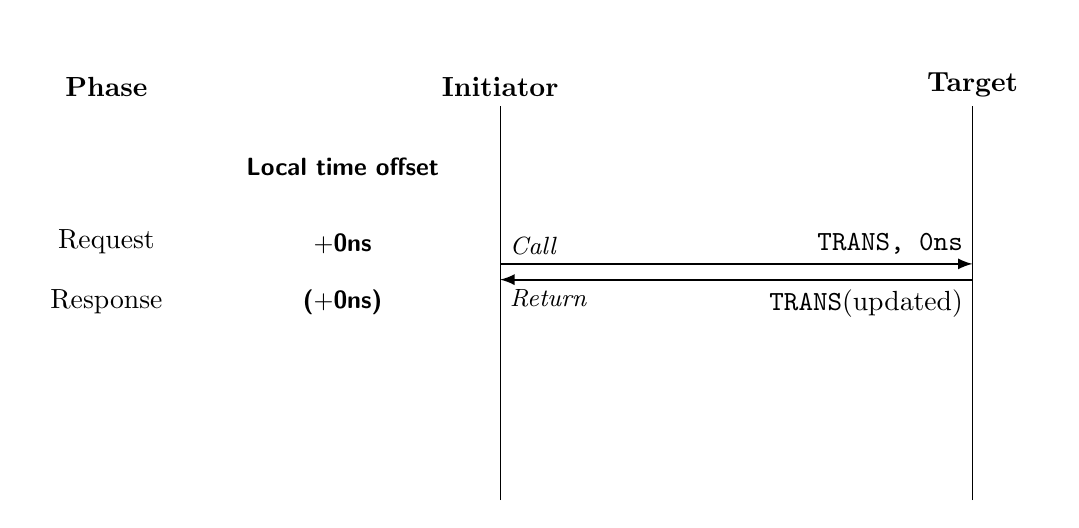
\begin{tikzpicture}
		\clip (1,0) rectangle (14,6);
%		\draw[help lines] (0,0) grid (15,10);
		\path (2,5) coordinate (phase);
		\path (2,3) coordinate (req);
		\path (2,2.8) coordinate (rsp);
		\path (5,4) coordinate (time);
		\path (5,3) coordinate (0ns);
		\path (5,2.8) coordinate (0nstext);
		\path (7,0) coordinate (llb);
		\path (7,5) coordinate (llt);
		\path (13,0) coordinate (rlb);
		\path (13,5) coordinate (rlt);
		\path (7,3) coordinate (call_left);
		\path (13,3) coordinate (call_right);
		\path (7,2.8) coordinate (ret_left);
		\path (13,2.8) coordinate (ret_right);

		\draw (phase) node[above] {\textbf{Phase}};
		\draw (llb) -- (llt)
			node[above] {\textbf{Initiator}};
		\draw (rlb) -- (rlt)
			node[above] {\textbf{Target}};
		\draw (req) node[above] {Request};
		\draw (rsp) node[below] {Response};
		\draw (time) node[above] {\small \textbf{\textsf{Local time offset}}};
		\draw (0ns) node[above] {\small \textbf{\textsf{$+$0ns}}};
		\draw (0nstext) node[below] {\small \textbf{\textsf{($+$0ns)}}};
		\draw[thick,-latex] (call_left) -- (call_right);
		\draw (call_left) node[above right] {\small \emph{Call}};
		\draw (call_right) node[above left] {\texttt{\textbf{TRANS, 0ns}}};
		\draw[thick,latex-] (ret_left) -- (ret_right);
		\draw (ret_left) node[below right] {\small \emph{Return}};
		\draw (ret_right) node[below left] {\texttt{\textbf{TRANS}}(updated)};
	\end{tikzpicture}
	\end{center}
	\caption{Untimed coding style message chart.}
	\label{fig:chart_untimed}
\end{figure}
}

\subsection{Loosely-timed with timing annotation}

\mode<presentation>{

\begin{frame}
	\frametitle{Loosely-timed with timing annotation}

\begin{figure}[h]
	\begin{center}
	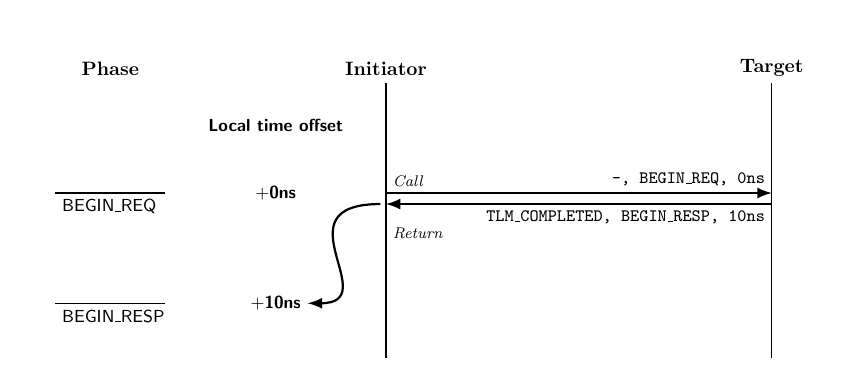
\begin{tikzpicture}[transform shape,scale=0.7]
		\clip (0.5,0) rectangle (15,6);
%		\draw[help lines] (0,0) grid (15,10);
		\path (2,5) coordinate (phase);
		\path (1,3) coordinate (req0);
		\path (3,3) coordinate (req1);
		\path (1,1) coordinate (rsp0);
		\path (3,1) coordinate (rsp1);
		\path (5,4) coordinate (time);
		\path (5,3) coordinate (0ns);
		\path (5,1) coordinate (10ns);
		\path (7,0) coordinate (llb);
		\path (7,5) coordinate (llt);
		\path (14,0) coordinate (rlb);
		\path (14,5) coordinate (rlt);
		\path (7,3) coordinate (call_left);
		\path (14,3) coordinate (call_right);
		\path (7,2.8) coordinate (ret_left);
		\path (14,2.8) coordinate (ret_right);

		\draw (phase) node[above] {\textbf{Phase}};
		\draw (llb) -- (llt)
			node[above] {\textbf{Initiator}};
		\draw (rlb) -- (rlt)
			node[above] {\textbf{Target}};
		\draw (req0) node[below right] {\small \textsf{BEGIN\_REQ}} -- (req1);
		\draw (rsp0) node[below right] {\small \textsf{BEGIN\_RESP}} -- (rsp1);
		\draw (time) node[above] {\small \textbf{\textsf{Local time offset}}};
		\draw (0ns) node {\small \textbf{\textsf{$+$0ns}}};
		\draw (10ns) node(10nstext) {\small \textbf{\textsf{$+$10ns}}};
		\draw[thick,-latex] (call_left) -- (call_right);
		\draw (call_left) node[above right] {\footnotesize \emph{Call}};
		\draw (call_right) node[above left] {\small \texttt{\textbf{-, BEGIN\_REQ, 0ns}}};
		\draw[thick,latex-] (ret_left) -- (ret_right);
		\draw (ret_left) +(0,-0.3) node[below right] {\footnotesize \emph{Return}};
		\draw (ret_right) node[below left] {\small \texttt{\textbf{TLM\_COMPLETED, BEGIN\_RESP, 10ns}}};
		\path (ret_left) +(-2,0) coordinate (control_ret_left);
		\path (10nstext)[above] +(2,0) coordinate (control_10nstext);
		\draw[thick,-latex] (ret_left) +(-0.1,0) .. controls (control_ret_left) and (control_10nstext) .. (10nstext)[above];
	\end{tikzpicture}
	\end{center}
\end{figure}

\end{frame}

}

\mode<article>{
Figure~\ref{fig:chart_lt_with_timing_annotation} shows the message exchange that occur when using the loosely-timed coding style with timing annotation.

\begin{figure}[h]
	\begin{center}
	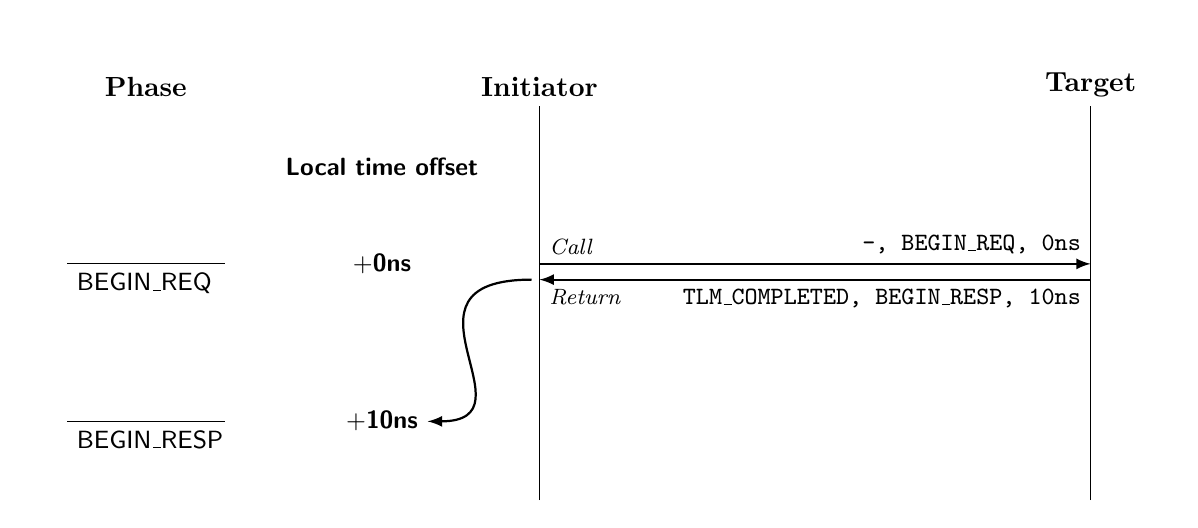
\begin{tikzpicture}
		\clip (0.5,0) rectangle (15,6);
%		\draw[help lines] (0,0) grid (15,10);
		\path (2,5) coordinate (phase);
		\path (1,3) coordinate (req0);
		\path (3,3) coordinate (req1);
		\path (1,1) coordinate (rsp0);
		\path (3,1) coordinate (rsp1);
		\path (5,4) coordinate (time);
		\path (5,3) coordinate (0ns);
		\path (5,1) coordinate (10ns);
		\path (7,0) coordinate (llb);
		\path (7,5) coordinate (llt);
		\path (14,0) coordinate (rlb);
		\path (14,5) coordinate (rlt);
		\path (7,3) coordinate (call_left);
		\path (14,3) coordinate (call_right);
		\path (7,2.8) coordinate (ret_left);
		\path (14,2.8) coordinate (ret_right);

		\draw (phase) node[above] {\textbf{Phase}};
		\draw (llb) -- (llt)
			node[above] {\textbf{Initiator}};
		\draw (rlb) -- (rlt)
			node[above] {\textbf{Target}};
		\draw (req0) node[below right] {\small \textsf{BEGIN\_REQ}} -- (req1);
		\draw (rsp0) node[below right] {\small \textsf{BEGIN\_RESP}} -- (rsp1);
		\draw (time) node[above] {\small \textbf{\textsf{Local time offset}}};
		\draw (0ns) node {\small \textbf{\textsf{$+$0ns}}};
		\draw (10ns) node(10nstext) {\small \textbf{\textsf{$+$10ns}}};
		\draw[thick,-latex] (call_left) -- (call_right);
		\draw (call_left) node[above right] {\footnotesize \emph{Call}};
		\draw (call_right) node[above left] {\small \texttt{\textbf{-, BEGIN\_REQ, 0ns}}};
		\draw[thick,latex-] (ret_left) -- (ret_right);
		\draw (ret_left) node[below right] {\footnotesize \emph{Return}};
		\draw (ret_right) node[below left] {\small \texttt{\textbf{TLM\_COMPLETED, BEGIN\_RESP, 10ns}}};
		\path (ret_left) +(-2,0) coordinate (control_ret_left);
		\path (10nstext)[above] +(2,0) coordinate (control_10nstext);
		\draw[thick,-latex] (ret_left) +(-0.1,0) .. controls (control_ret_left) and (control_10nstext) .. (10nstext)[above];
	\end{tikzpicture}
	\end{center}
	\caption{Loosely-timed coding style with timing annotation message chart.}
	\label{fig:chart_lt_with_timing_annotation}
\end{figure}
}

\clearpage
\subsection{Loosely-timed with sync}

\mode<presentation>{

\begin{frame}
	\frametitle{Loosely-timed with sync}

\begin{figure}[h]
	\begin{center}
	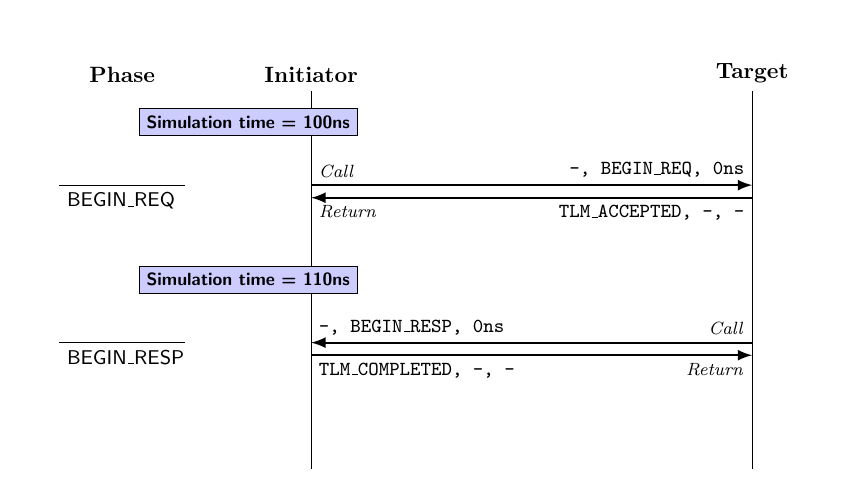
\begin{tikzpicture}[transform shape,scale=0.8]
		\clip (2.5,0) rectangle (15,7);
%		\draw[help lines] (0,0) grid (15,10);
		\path (4,6) coordinate (phase);
		\path (3,4.5) coordinate (req0);
		\path (5,4.5) coordinate (req1);
		\path (3,2) coordinate (rsp0);
		\path (5,2) coordinate (rsp1);
		\path (7,0) coordinate (llb);
		\path (7,6) coordinate (llt);
		\path (14,0) coordinate (rlb);
		\path (14,6) coordinate (rlt);
		\path (7,4.5) coordinate (call_left);
		\path (14,4.5) coordinate (call_right);
		\path (7,4.3) coordinate (ret_left);
		\path (14,4.3) coordinate (ret_right);
		\path (7,2) coordinate (call2_left);
		\path (14,2) coordinate (call2_right);
		\path (7,1.8) coordinate (ret2_left);
		\path (14,1.8) coordinate (ret2_right);

		\draw (phase) node[above] {\textbf{Phase}};
		\draw (llb) -- (llt)
			node[above] {\textbf{Initiator}};
		\draw (rlb) -- (rlt)
			node[above] {\textbf{Target}};
		\draw (req0) node[below right] {\small \textsf{BEGIN\_REQ}} -- (req1);
		\draw (rsp0) node[below right] {\small \textsf{BEGIN\_RESP}} -- (rsp1);
		\draw[thick,-latex] (call_left) -- (call_right);
		\draw (call_left) node[above right] {\footnotesize \emph{Call}};
		\draw (call_right) node[above left] {\small \texttt{\textbf{-, BEGIN\_REQ, 0ns}}};
		\draw[thick,latex-] (ret_left) -- (ret_right);
		\draw (ret_left) node[below right] {\footnotesize \emph{Return}};
		\draw (ret_right) node[below left] {\small \texttt{\textbf{TLM\_ACCEPTED, -, -}}};
		\draw[thick,latex-] (call2_left) -- (call2_right);
		\draw (call2_right) node[above left] {\footnotesize \emph{Call}};
		\draw (call2_left) node[above right] {\small \texttt{\textbf{-, BEGIN\_RESP, 0ns}}};
		\draw[thick,-latex] (ret2_left) -- (ret2_right);
		\draw (ret2_right) node[below left] {\footnotesize \emph{Return}};
		\draw (ret2_left) node[below right] {\small \texttt{\textbf{TLM\_COMPLETED, -, -}}};
		\path (6,5.5) node(100ns) [rectangle,draw,fill=blue!20] {\footnotesize \textsf{\textbf{Simulation time = 100ns}}};
		\path (6,3) node(110ns) [rectangle,draw,fill=blue!20] {\footnotesize \textsf{\textbf{Simulation time = 110ns}}};
	\end{tikzpicture}
	\end{center}
\end{figure}
\end{frame}
}

\mode<article>{
Figure~\ref{fig:chart_lt_with_sync} shows the message exchange that occur when using the loosely-timed coding style with sync.

\begin{figure}[h]
	\begin{center}
	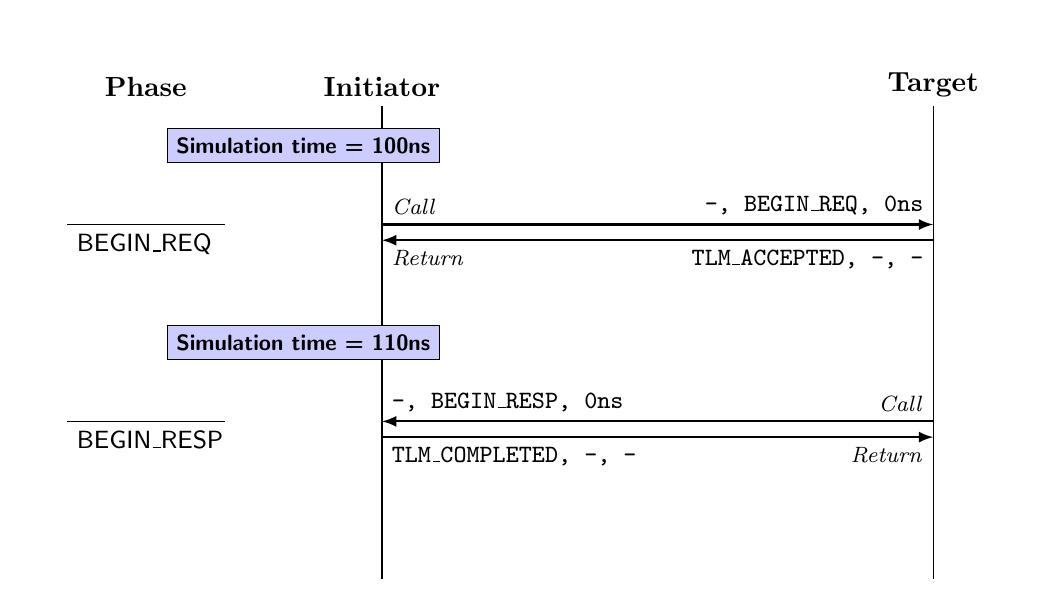
\begin{tikzpicture}
		\clip (2.5,0) rectangle (15,7);
%		\draw[help lines] (0,0) grid (15,10);
		\path (4,6) coordinate (phase);
		\path (3,4.5) coordinate (req0);
		\path (5,4.5) coordinate (req1);
		\path (3,2) coordinate (rsp0);
		\path (5,2) coordinate (rsp1);
		\path (7,0) coordinate (llb);
		\path (7,6) coordinate (llt);
		\path (14,0) coordinate (rlb);
		\path (14,6) coordinate (rlt);
		\path (7,4.5) coordinate (call_left);
		\path (14,4.5) coordinate (call_right);
		\path (7,4.3) coordinate (ret_left);
		\path (14,4.3) coordinate (ret_right);
		\path (7,2) coordinate (call2_left);
		\path (14,2) coordinate (call2_right);
		\path (7,1.8) coordinate (ret2_left);
		\path (14,1.8) coordinate (ret2_right);

		\draw (phase) node[above] {\textbf{Phase}};
		\draw (llb) -- (llt)
			node[above] {\textbf{Initiator}};
		\draw (rlb) -- (rlt)
			node[above] {\textbf{Target}};
		\draw (req0) node[below right] {\small \textsf{BEGIN\_REQ}} -- (req1);
		\draw (rsp0) node[below right] {\small \textsf{BEGIN\_RESP}} -- (rsp1);
		\draw[thick,-latex] (call_left) -- (call_right);
		\draw (call_left) node[above right] {\footnotesize \emph{Call}};
		\draw (call_right) node[above left] {\small \texttt{\textbf{-, BEGIN\_REQ, 0ns}}};
		\draw[thick,latex-] (ret_left) -- (ret_right);
		\draw (ret_left) node[below right] {\footnotesize \emph{Return}};
		\draw (ret_right) node[below left] {\small \texttt{\textbf{TLM\_ACCEPTED, -, -}}};
		\draw[thick,latex-] (call2_left) -- (call2_right);
		\draw (call2_right) node[above left] {\footnotesize \emph{Call}};
		\draw (call2_left) node[above right] {\small \texttt{\textbf{-, BEGIN\_RESP, 0ns}}};
		\draw[thick,-latex] (ret2_left) -- (ret2_right);
		\draw (ret2_right) node[below left] {\footnotesize \emph{Return}};
		\draw (ret2_left) node[below right] {\small \texttt{\textbf{TLM\_COMPLETED, -, -}}};
		\path (6,5.5) node(100ns) [rectangle,draw,fill=blue!20] {\footnotesize \textsf{\textbf{Simulation time = 100ns}}};
		\path (6,3) node(110ns) [rectangle,draw,fill=blue!20] {\footnotesize \textsf{\textbf{Simulation time = 110ns}}};
	\end{tikzpicture}
	\end{center}
	\caption{Loosely-timed coding style with sync message chart.}
	\label{fig:chart_lt_with_sync}
\end{figure}
}

\clearpage
\subsection{Loosely-timed with temporal decoupling}

\mode<presentation>{

\begin{frame}
	\frametitle{Loosely-timed with temporal decoupling}

\begin{figure}[h]
	\begin{center}
	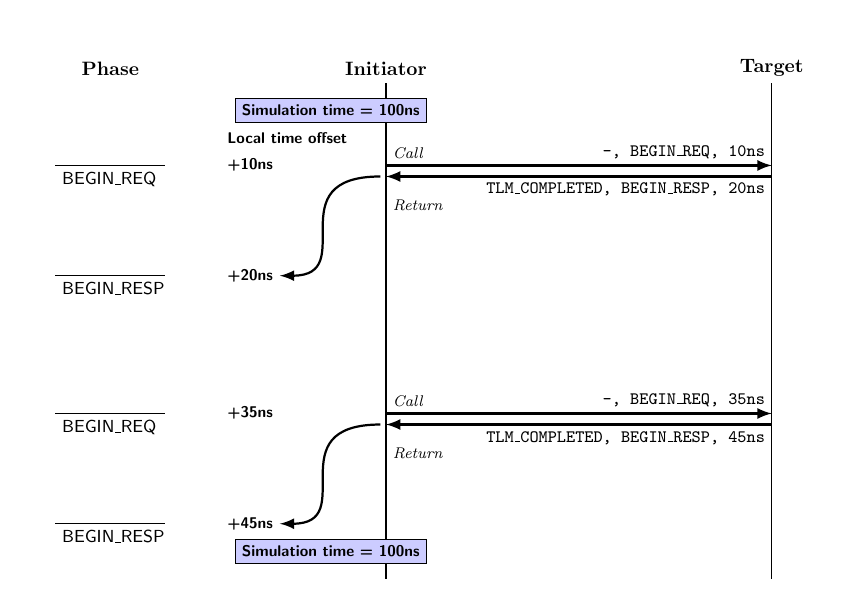
\begin{tikzpicture}[transform shape,scale=0.7]
		\clip (0.5,0) rectangle (15,10);
%		\draw[help lines] (0,0) grid (15,10);
		\path (2,9) coordinate (phase);
		\path (1,7.5) coordinate (req0);
		\path (3,7.5) coordinate (req1);
		\path (1,5.5) coordinate (rsp0);
		\path (3,5.5) coordinate (rsp1);
		\path (1,3) coordinate (req1_0);
		\path (3,3) coordinate (req1_1);
		\path (1,1) coordinate (rsp1_0);
		\path (3,1) coordinate (rsp1_1);
		\path (4,8) node(local_time) [right] {\footnotesize \textsf{\textbf{Local time offset}}};
		\path (4,7.5) node(10ns) [right] {\footnotesize \textsf{\textbf{+10ns}}};
		\path (4,5.5) node(20ns) [right] {\footnotesize \textsf{\textbf{+20ns}}};
		\path (4,3) node(35ns) [right] {\footnotesize \textsf{\textbf{+35ns}}};
		\path (4,1) node(45ns) [right] {\footnotesize \textsf{\textbf{+45ns}}};
		\path (7,0) coordinate (llb);
		\path (7,9) coordinate (llt);
		\path (14,0) coordinate (rlb);
		\path (14,9) coordinate (rlt);
		\path (7,7.5) coordinate (call_left);
		\path (14,7.5) coordinate (call_right);
		\path (7,7.3) coordinate (ret_left);
		\path (14,7.3) coordinate (ret_right);
		\path (7,3) coordinate (call2_left);
		\path (14,3) coordinate (call2_right);
		\path (7,2.8) coordinate (ret2_left);
		\path (14,2.8) coordinate (ret2_right);

		\draw (phase) node[above] {\textbf{Phase}};
		\draw (llb) -- (llt)
			node[above] {\textbf{Initiator}};
		\draw (rlb) -- (rlt)
			node[above] {\textbf{Target}};
		\draw (req0) node[below right] {\small \textsf{BEGIN\_REQ}} -- (req1);
		\draw (rsp0) node[below right] {\small \textsf{BEGIN\_RESP}} -- (rsp1);
		\draw (req1_0) node[below right] {\small \textsf{BEGIN\_REQ}} -- (req1_1);
		\draw (rsp1_0) node[below right] {\small \textsf{BEGIN\_RESP}} -- (rsp1_1);
		\draw[thick,-latex] (call_left) -- (call_right);
		\draw (call_left) node[above right] {\footnotesize \emph{Call}};
		\draw (call_right) node[above left] {\small \texttt{\textbf{-, BEGIN\_REQ, 10ns}}};
		\draw[thick,latex-] (ret_left) -- (ret_right);
		\draw (ret_left) +(0,-0.3) node[below right] {\footnotesize \emph{Return}};
		\draw (ret_right) node[below left] {\small \texttt{\textbf{TLM\_COMPLETED, BEGIN\_RESP, 20ns}}};
		\draw[thick,-latex] (call2_left) -- (call2_right);
		\draw (call2_left) node[above right] {\footnotesize \emph{Call}};
		\draw (call2_right) node[above left] {\small \texttt{\textbf{-, BEGIN\_REQ, 35ns}}};
		\draw[thick,latex-] (ret2_left) -- (ret2_right);
		\draw (ret2_left) +(0,-0.3) node[below right] {\footnotesize \emph{Return}};
		\draw (ret2_right) node[below left] {\small \texttt{\textbf{TLM\_COMPLETED, BEGIN\_RESP, 45ns}}};
		\path (6,8.5) node(100ns) [rectangle,draw,fill=blue!20] {\footnotesize \textsf{\textbf{Simulation time = 100ns}}};
		\path (6,0.5) node(100_ns) [rectangle,draw,fill=blue!20] {\footnotesize \textsf{\textbf{Simulation time = 100ns}}};
		\path (ret_left) +(-2,0) coordinate (control_ret_left);
		\path (20ns) +(2,0) coordinate (control_20ns);
		\draw[thick,-latex] (ret_left) +(-0.1,0) .. controls (control_ret_left) and (control_20ns) .. (20ns)[above];
		\path (ret2_left) +(-2,0) coordinate (control_ret2_left);
		\path (45ns) +(2,0) coordinate (control_45ns);
		\draw[thick,-latex] (ret2_left) +(-0.1,0) .. controls (control_ret2_left) and (control_45ns) .. (45ns)[above];
	\end{tikzpicture}
	\end{center}
\end{figure}
\end{frame}

}

\mode<article>{
Figure~\ref{fig:chart_lt_with_temporal_decoupling} shows the message exchange that occur when using the loosely-timed coding style with temporal decoupling.

\begin{figure}[h]
	\begin{center}
	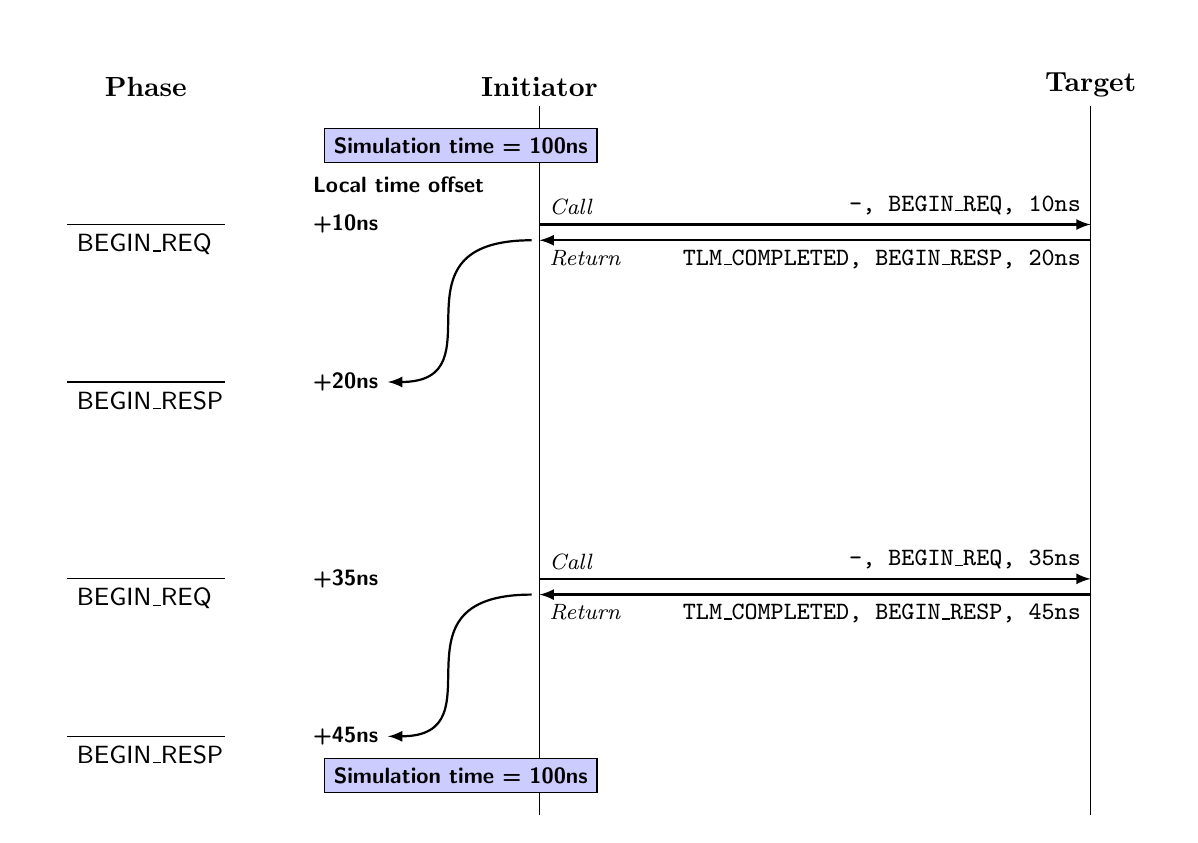
\begin{tikzpicture}
		\clip (0.5,0) rectangle (15,10);
%		\draw[help lines] (0,0) grid (15,10);
		\path (2,9) coordinate (phase);
		\path (1,7.5) coordinate (req0);
		\path (3,7.5) coordinate (req1);
		\path (1,5.5) coordinate (rsp0);
		\path (3,5.5) coordinate (rsp1);
		\path (1,3) coordinate (req1_0);
		\path (3,3) coordinate (req1_1);
		\path (1,1) coordinate (rsp1_0);
		\path (3,1) coordinate (rsp1_1);
		\path (4,8) node(local_time) [right] {\footnotesize \textsf{\textbf{Local time offset}}};
		\path (4,7.5) node(10ns) [right] {\footnotesize \textsf{\textbf{+10ns}}};
		\path (4,5.5) node(20ns) [right] {\footnotesize \textsf{\textbf{+20ns}}};
		\path (4,3) node(35ns) [right] {\footnotesize \textsf{\textbf{+35ns}}};
		\path (4,1) node(45ns) [right] {\footnotesize \textsf{\textbf{+45ns}}};
		\path (7,0) coordinate (llb);
		\path (7,9) coordinate (llt);
		\path (14,0) coordinate (rlb);
		\path (14,9) coordinate (rlt);
		\path (7,7.5) coordinate (call_left);
		\path (14,7.5) coordinate (call_right);
		\path (7,7.3) coordinate (ret_left);
		\path (14,7.3) coordinate (ret_right);
		\path (7,3) coordinate (call2_left);
		\path (14,3) coordinate (call2_right);
		\path (7,2.8) coordinate (ret2_left);
		\path (14,2.8) coordinate (ret2_right);

		\draw (phase) node[above] {\textbf{Phase}};
		\draw (llb) -- (llt)
			node[above] {\textbf{Initiator}};
		\draw (rlb) -- (rlt)
			node[above] {\textbf{Target}};
		\draw (req0) node[below right] {\small \textsf{BEGIN\_REQ}} -- (req1);
		\draw (rsp0) node[below right] {\small \textsf{BEGIN\_RESP}} -- (rsp1);
		\draw (req1_0) node[below right] {\small \textsf{BEGIN\_REQ}} -- (req1_1);
		\draw (rsp1_0) node[below right] {\small \textsf{BEGIN\_RESP}} -- (rsp1_1);
		\draw[thick,-latex] (call_left) -- (call_right);
		\draw (call_left) node[above right] {\footnotesize \emph{Call}};
		\draw (call_right) node[above left] {\small \texttt{\textbf{-, BEGIN\_REQ, 10ns}}};
		\draw[thick,latex-] (ret_left) -- (ret_right);
		\draw (ret_left) node[below right] {\footnotesize \emph{Return}};
		\draw (ret_right) node[below left] {\small \texttt{\textbf{TLM\_COMPLETED, BEGIN\_RESP, 20ns}}};
		\draw[thick,-latex] (call2_left) -- (call2_right);
		\draw (call2_left) node[above right] {\footnotesize \emph{Call}};
		\draw (call2_right) node[above left] {\small \texttt{\textbf{-, BEGIN\_REQ, 35ns}}};
		\draw[thick,latex-] (ret2_left) -- (ret2_right);
		\draw (ret2_left) node[below right] {\footnotesize \emph{Return}};
		\draw (ret2_right) node[below left] {\small \texttt{\textbf{TLM\_COMPLETED, BEGIN\_RESP, 45ns}}};
		\path (6,8.5) node(100ns) [rectangle,draw,fill=blue!20] {\footnotesize \textsf{\textbf{Simulation time = 100ns}}};
		\path (6,0.5) node(100_ns) [rectangle,draw,fill=blue!20] {\footnotesize \textsf{\textbf{Simulation time = 100ns}}};
		\path (ret_left) +(-2,0) coordinate (control_ret_left);
		\path (20ns) +(2,0) coordinate (control_20ns);
		\draw[thick,-latex] (ret_left) +(-0.1,0) .. controls (control_ret_left) and (control_20ns) .. (20ns)[above];
		\path (ret2_left) +(-2,0) coordinate (control_ret2_left);
		\path (45ns) +(2,0) coordinate (control_45ns);
		\draw[thick,-latex] (ret2_left) +(-0.1,0) .. controls (control_ret2_left) and (control_45ns) .. (45ns)[above];
	\end{tikzpicture}
	\end{center}
	\caption{Loosely-timed coding style with temporal decoupling message chart.}
	\label{fig:chart_lt_with_temporal_decoupling}
\end{figure}
}

\clearpage
\subsection{Loosely-timed with temporal decoupling and synchronization-on-demand}

\mode<presentation>{

\begin{frame}
	\frametitle{\scriptsize Loosely-timed with temporal decoupling and synchronization-on-demand}

\begin{figure}[h]
	\begin{center}
	\begin{tikzpicture}[transform shape,scale=0.7]
		\clip (0.5,0) rectangle (15,10);
%		\draw[help lines] (0,0) grid (15,10);
		\path (2,9) coordinate (phase);
		\path (1,7.5) coordinate (req0);
		\path (3,7.5) coordinate (req1);
		\path (1,4) coordinate (rsp0);
		\path (3,4) coordinate (rsp1);
		\path (1,2) coordinate (req1_0);
		\path (3,2) coordinate (req1_1);
		\path (1,1) coordinate (rsp1_0);
		\path (3,1) coordinate (rsp1_1);
		\path (4,8) node(local_time) [right] {\footnotesize \textsf{\textbf{Local time offset}}};
		\path (4,7.5) node(10ns) [right] {\footnotesize \textsf{\textbf{+10ns}}};
		\path (4,6.5) node(wait) [right] {\footnotesize \textsf{\textbf{wait(\ldots)}}};
		\path (4,4) node(0s) [right] {\footnotesize \textsf{\textbf{+0ns}}};
		\path (4,2) node(20ns) [right] {\footnotesize \textsf{\textbf{+20ns}}};
		\path (4,1) node(30ns) [right] {\footnotesize \textsf{\textbf{+30ns}}};
		\path (7,0) coordinate (llb);
		\path (7,9) coordinate (llt);
		\path (14,0) coordinate (rlb);
		\path (14,9) coordinate (rlt);
		\path (7,7.5) coordinate (call_left);
		\path (14,7.5) coordinate (call_right);
		\path (7,7.3) coordinate (ret_left);
		\path (14,7.3) coordinate (ret_right);
		\path (7,4) coordinate (call2_left);
		\path (14,4) coordinate (call2_right);
		\path (7,3.8) coordinate (ret2_left);
		\path (14,3.8) coordinate (ret2_right);
		\path (7,2) coordinate (call3_left);
		\path (14,2) coordinate (call3_right);
		\path (7,1.8) coordinate (ret3_left);
		\path (14,1.8) coordinate (ret3_right);

		\draw (phase) node[above] {\textbf{Phase}};
		\draw (llb) -- (llt)
			node[above] {\textbf{Initiator}};
		\draw (rlb) -- (rlt)
			node[above] {\textbf{Target}};
		\draw (req0) node[below right] {\small \textsf{BEGIN\_REQ}} -- (req1);
		\draw (rsp0) node[below right] {\small \textsf{BEGIN\_RESP}} -- (rsp1);
		\draw (req1_0) node[below right] {\small \textsf{BEGIN\_REQ}} -- (req1_1);
		\draw (rsp1_0) node[below right] {\small \textsf{BEGIN\_RESP}} -- (rsp1_1);
		\draw[thick,-latex] (call_left) -- (call_right);
		\draw (call_left) node[above right] {\footnotesize \emph{Call}};
		\draw (call_right) node[above left] {\small \texttt{\textbf{-, BEGIN\_REQ, 10ns}}};
		\draw[thick,latex-] (ret_left) -- (ret_right);
		\draw (ret_left) node[below right] {\footnotesize \emph{Return}};
		\draw (ret_right) node[below left] {\small \texttt{\textbf{TLM\_ACCEPTED, -, -}}};
		\draw[thick,latex-] (call2_left) -- (call2_right);
		\draw (call2_right) node[above left] {\footnotesize \emph{Call}};
		\draw (call2_left) node[above right] {\small \texttt{\textbf{-, BEGIN\_RESP, 0ns}}};
		\draw[thick,-latex] (ret2_left) -- (ret2_right);
		\draw (ret2_right) node[below left] {\footnotesize \emph{Return}};
		\draw (ret2_left) node[below right] {\small \texttt{\textbf{TLM\_COMPLETED, -, -}}};
		\draw[thick,-latex] (call3_left) -- (call3_right);
		\draw (call3_left) node[above right] {\footnotesize \emph{Call}};
		\draw (call3_right) node[above left] {\small \texttt{\textbf{-, BEGIN\_REQ, 20ns}}};
		\draw[thick,latex-] (ret3_left) -- (ret3_right);
		\draw (ret3_left) +(0,-0.3) node[below right] {\footnotesize \emph{Return}};
		\draw (ret3_right) node[below left] {\small \texttt{\textbf{TLM\_COMPLETED, BEGIN\_RESP, 30ns}}};
		\path (6,8.5) node(5us) [rectangle,draw,fill=blue!20] {\footnotesize \textsf{\textbf{Simulation time = 5us}}};
		\path (6,5.5) node(6us1) [rectangle,draw,fill=blue!20] {\footnotesize \textsf{\textbf{Simulation time = 6us}}};
		\path (6,0.25) node(6us2) [rectangle,draw,fill=blue!20] {\footnotesize \textsf{\textbf{Simulation time = 6us}}};
		\path (ret_left) +(-1.5,0) coordinate (control_ret_left);
		\path (wait) +(1.5,0) coordinate (control_wait);
		\draw[thick,-latex] (ret_left) +(-0.1,0) .. controls (control_ret_left) and (control_wait) .. (wait)[above];
		\path (ret3_left) +(-2,0) coordinate (control_ret3_left);
		\path (45ns) +(2,0) coordinate (control_45ns);
		\draw[thick,-latex] (ret3_left) +(-0.1,0) .. controls (control_ret3_left) and (control_45ns) .. (45ns)[above];
	\end{tikzpicture}
	\end{center}
\end{figure}

\end{frame}

}

\mode<article>{
Figure~\ref{fig:chart_lt_with_temporal_decoupling_and_sync_on_demand} shows the message exchange that occur when using the loosely-timed coding style with temporal decoupling and synchronization-on-demand.

\begin{figure}[h]
	\begin{center}
	\begin{tikzpicture}
		\clip (0.5,0) rectangle (15,10);
%		\draw[help lines] (0,0) grid (15,10);
		\path (2,9) coordinate (phase);
		\path (1,7.5) coordinate (req0);
		\path (3,7.5) coordinate (req1);
		\path (1,4) coordinate (rsp0);
		\path (3,4) coordinate (rsp1);
		\path (1,2) coordinate (req1_0);
		\path (3,2) coordinate (req1_1);
		\path (1,1) coordinate (rsp1_0);
		\path (3,1) coordinate (rsp1_1);
		\path (4,8) node(local_time) [right] {\footnotesize \textsf{\textbf{Local time offset}}};
		\path (4,7.5) node(10ns) [right] {\footnotesize \textsf{\textbf{+10ns}}};
		\path (4,6.5) node(wait) [right] {\footnotesize \textsf{\textbf{wait(\ldots)}}};
		\path (4,4) node(0s) [right] {\footnotesize \textsf{\textbf{+0ns}}};
		\path (4,2) node(20ns) [right] {\footnotesize \textsf{\textbf{+20ns}}};
		\path (4,1) node(30ns) [right] {\footnotesize \textsf{\textbf{+30ns}}};
		\path (7,0) coordinate (llb);
		\path (7,9) coordinate (llt);
		\path (14,0) coordinate (rlb);
		\path (14,9) coordinate (rlt);
		\path (7,7.5) coordinate (call_left);
		\path (14,7.5) coordinate (call_right);
		\path (7,7.3) coordinate (ret_left);
		\path (14,7.3) coordinate (ret_right);
		\path (7,4) coordinate (call2_left);
		\path (14,4) coordinate (call2_right);
		\path (7,3.8) coordinate (ret2_left);
		\path (14,3.8) coordinate (ret2_right);
		\path (7,2) coordinate (call3_left);
		\path (14,2) coordinate (call3_right);
		\path (7,1.8) coordinate (ret3_left);
		\path (14,1.8) coordinate (ret3_right);

		\draw (phase) node[above] {\textbf{Phase}};
		\draw (llb) -- (llt)
			node[above] {\textbf{Initiator}};
		\draw (rlb) -- (rlt)
			node[above] {\textbf{Target}};
		\draw (req0) node[below right] {\small \textsf{BEGIN\_REQ}} -- (req1);
		\draw (rsp0) node[below right] {\small \textsf{BEGIN\_RESP}} -- (rsp1);
		\draw (req1_0) node[below right] {\small \textsf{BEGIN\_REQ}} -- (req1_1);
		\draw (rsp1_0) node[below right] {\small \textsf{BEGIN\_RESP}} -- (rsp1_1);
		\draw[thick,-latex] (call_left) -- (call_right);
		\draw (call_left) node[above right] {\footnotesize \emph{Call}};
		\draw (call_right) node[above left] {\small \texttt{\textbf{-, BEGIN\_REQ, 10ns}}};
		\draw[thick,latex-] (ret_left) -- (ret_right);
		\draw (ret_left) node[below right] {\footnotesize \emph{Return}};
		\draw (ret_right) node[below left] {\small \texttt{\textbf{TLM\_ACCEPTED, -, -}}};
		\draw[thick,latex-] (call2_left) -- (call2_right);
		\draw (call2_right) node[above left] {\footnotesize \emph{Call}};
		\draw (call2_left) node[above right] {\small \texttt{\textbf{-, BEGIN\_RESP, 0ns}}};
		\draw[thick,-latex] (ret2_left) -- (ret2_right);
		\draw (ret2_right) node[below left] {\footnotesize \emph{Return}};
		\draw (ret2_left) node[below right] {\small \texttt{\textbf{TLM\_COMPLETED, -, -}}};
		\draw[thick,-latex] (call3_left) -- (call3_right);
		\draw (call3_left) node[above right] {\footnotesize \emph{Call}};
		\draw (call3_right) node[above left] {\small \texttt{\textbf{-, BEGIN\_REQ, 20ns}}};
		\draw[thick,latex-] (ret3_left) -- (ret3_right);
		\draw (ret3_left) node[below right] {\footnotesize \emph{Return}};
		\draw (ret3_right) node[below left] {\small \texttt{\textbf{TLM\_COMPLETED, BEGIN\_RESP, 30ns}}};
		\path (6,8.5) node(5us) [rectangle,draw,fill=blue!20] {\footnotesize \textsf{\textbf{Simulation time = 5us}}};
		\path (6,5.5) node(6us1) [rectangle,draw,fill=blue!20] {\footnotesize \textsf{\textbf{Simulation time = 6us}}};
		\path (6,0.25) node(6us2) [rectangle,draw,fill=blue!20] {\footnotesize \textsf{\textbf{Simulation time = 6us}}};
		\path (ret_left) +(-1.5,0) coordinate (control_ret_left);
		\path (wait) +(1.5,0) coordinate (control_wait);
		\draw[thick,-latex] (ret_left) +(-0.1,0) .. controls (control_ret_left) and (control_wait) .. (wait)[above];
		\path (ret3_left) +(-2,0) coordinate (control_ret3_left);
		\path (45ns) +(2,0) coordinate (control_45ns);
		\draw[thick,-latex] (ret3_left) +(-0.1,0) .. controls (control_ret3_left) and (control_45ns) .. (45ns)[above];
	\end{tikzpicture}
	\end{center}
	\caption{Loosely-timed coding style with temporal decoupling and synchronization-on-demand message chart.}
	\label{fig:chart_lt_with_temporal_decoupling_and_sync_on_demand}
\end{figure}
}

\clearpage
\subsection{Loosely-timed with temporal decoupling and quantum}

\mode<presentation>{

\begin{frame}
	\frametitle{\small Loosely-timed with temporal decoupling and quantum}

\begin{figure}[h]
	\begin{center}
	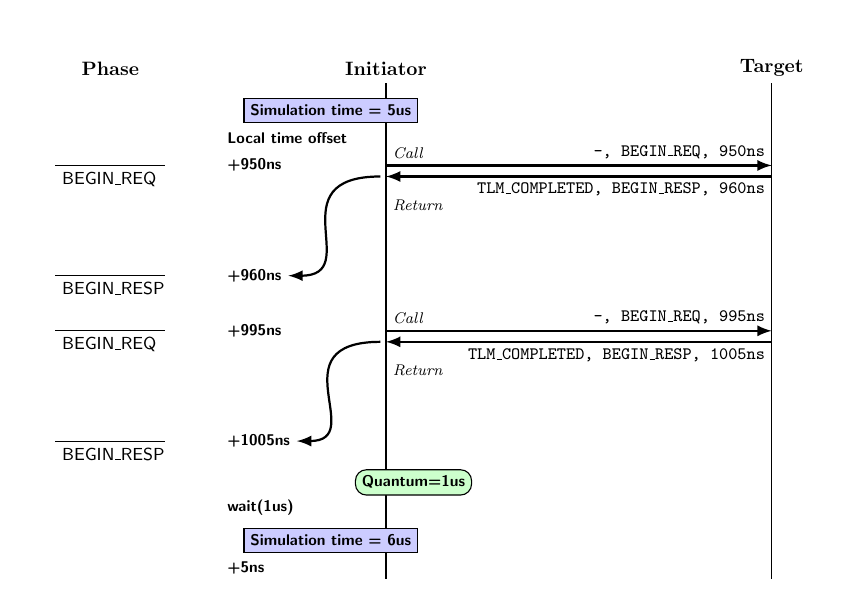
\begin{tikzpicture}[transform shape,scale=0.7]
		\clip (0.5,0) rectangle (15,10);
%		\draw[help lines] (0,0) grid (15,10);
		\path (2,9) coordinate (phase);
		\path (1,7.5) coordinate (req0);
		\path (3,7.5) coordinate (req1);
		\path (1,5.5) coordinate (rsp0);
		\path (3,5.5) coordinate (rsp1);
		\path (1,4.5) coordinate (req1_0);
		\path (3,4.5) coordinate (req1_1);
		\path (1,2.5) coordinate (rsp1_0);
		\path (3,2.5) coordinate (rsp1_1);
		\path (4,8) node(local_time) [right] {\footnotesize \textsf{\textbf{Local time offset}}};
		\path (4,7.5) node(10ns) [right] {\footnotesize \textsf{\textbf{+950ns}}};
		\path (4,5.5) node(20ns) [right] {\footnotesize \textsf{\textbf{+960ns}}};
		\path (4,4.5) node(35ns) [right] {\footnotesize \textsf{\textbf{+995ns}}};
		\path (4,2.5) node(45ns) [right] {\footnotesize \textsf{\textbf{+1005ns}}};
		\path (4,1.3) node(wait) [right] {\footnotesize \textsf{\textbf{wait(1us)}}};
		\path (4,0.2) node(5ns) [right] {\footnotesize \textsf{\textbf{+5ns}}};
		\path (7,0) coordinate (llb);
		\path (7,9) coordinate (llt);
		\path (14,0) coordinate (rlb);
		\path (14,9) coordinate (rlt);
		\path (7,7.5) coordinate (call_left);
		\path (14,7.5) coordinate (call_right);
		\path (7,7.3) coordinate (ret_left);
		\path (14,7.3) coordinate (ret_right);
		\path (7,4.5) coordinate (call2_left);
		\path (14,4.5) coordinate (call2_right);
		\path (7,4.3) coordinate (ret2_left);
		\path (14,4.3) coordinate (ret2_right);

		\draw (phase) node[above] {\textbf{Phase}};
		\draw (llb) -- (llt)
			node[above] {\textbf{Initiator}};
		\draw (rlb) -- (rlt)
			node[above] {\textbf{Target}};
		\draw (req0) node[below right] {\small \textsf{BEGIN\_REQ}} -- (req1);
		\draw (rsp0) node[below right] {\small \textsf{BEGIN\_RESP}} -- (rsp1);
		\draw (req1_0) node[below right] {\small \textsf{BEGIN\_REQ}} -- (req1_1);
		\draw (rsp1_0) node[below right] {\small \textsf{BEGIN\_RESP}} -- (rsp1_1);
		\draw[thick,-latex] (call_left) -- (call_right);
		\draw (call_left) node[above right] {\footnotesize \emph{Call}};
		\draw (call_right) node[above left] {\small \texttt{\textbf{-, BEGIN\_REQ, 950ns}}};
		\draw[thick,latex-] (ret_left) -- (ret_right);
		\draw (ret_left) +(0,-0.3) node[below right] {\footnotesize \emph{Return}};
		\draw (ret_right) node[below left] {\small \texttt{\textbf{TLM\_COMPLETED, BEGIN\_RESP, 960ns}}};
		\draw[thick,-latex] (call2_left) -- (call2_right);
		\draw (call2_left) node[above right] {\footnotesize \emph{Call}};
		\draw (call2_right) node[above left] {\small \texttt{\textbf{-, BEGIN\_REQ, 995ns}}};
		\draw[thick,latex-] (ret2_left) -- (ret2_right);
		\draw (ret2_left) +(0,-0.3) node[below right] {\footnotesize \emph{Return}};
		\draw (ret2_right) node[below left] {\small \texttt{\textbf{TLM\_COMPLETED, BEGIN\_RESP, 1005ns}}};
		\path (6,8.5) node(100ns) [rectangle,draw,fill=blue!20] {\footnotesize \textsf{\textbf{Simulation time = 5us}}};
		\path (6,0.7) node(110ns) [rectangle,draw,fill=blue!20] {\footnotesize \textsf{\textbf{Simulation time = 6us}}};
		\path (7.5,1.75) node(quantum) [rectangle,rounded corners,draw,fill=green!20] {\footnotesize \textsf{\textbf{Quantum=1us}}};
		\path (ret_left) +(-2,0) coordinate (control_ret_left);
		\path (20ns) +(2,0) coordinate (control_20ns);
		\draw[thick,-latex] (ret_left) +(-0.1,0) .. controls (control_ret_left) and (control_20ns) .. (20ns)[above];
		\path (ret2_left) +(-2,0) coordinate (control_ret2_left);
		\path (45ns) +(2,0) coordinate (control_45ns);
		\draw[thick,-latex] (ret2_left) +(-0.1,0) .. controls (control_ret2_left) and (control_45ns) .. (45ns)[above];
	\end{tikzpicture}
	\end{center}
\end{figure}
\end{frame}

}

\mode<article>{
Figure~\ref{fig:chart_lt_with_temporal_decoupling_and_quantum} shows the message exchange that occur when using the loosely-timed coding style and quantum.

\begin{figure}[h]
	\begin{center}
	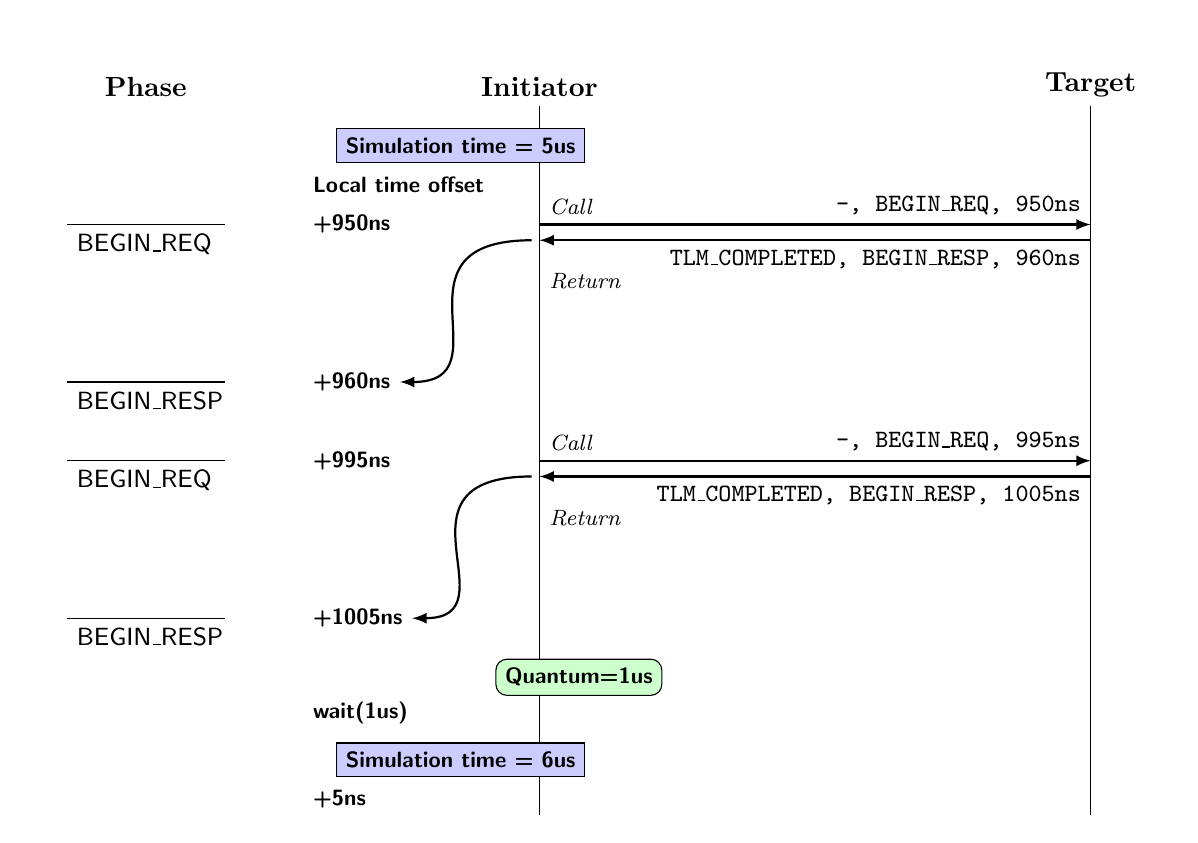
\begin{tikzpicture}
		\clip (0.5,0) rectangle (15,10);
%		\draw[help lines] (0,0) grid (15,10);
		\path (2,9) coordinate (phase);
		\path (1,7.5) coordinate (req0);
		\path (3,7.5) coordinate (req1);
		\path (1,5.5) coordinate (rsp0);
		\path (3,5.5) coordinate (rsp1);
		\path (1,4.5) coordinate (req1_0);
		\path (3,4.5) coordinate (req1_1);
		\path (1,2.5) coordinate (rsp1_0);
		\path (3,2.5) coordinate (rsp1_1);
		\path (4,8) node(local_time) [right] {\footnotesize \textsf{\textbf{Local time offset}}};
		\path (4,7.5) node(10ns) [right] {\footnotesize \textsf{\textbf{+950ns}}};
		\path (4,5.5) node(20ns) [right] {\footnotesize \textsf{\textbf{+960ns}}};
		\path (4,4.5) node(35ns) [right] {\footnotesize \textsf{\textbf{+995ns}}};
		\path (4,2.5) node(45ns) [right] {\footnotesize \textsf{\textbf{+1005ns}}};
		\path (4,1.3) node(wait) [right] {\footnotesize \textsf{\textbf{wait(1us)}}};
		\path (4,0.2) node(5ns) [right] {\footnotesize \textsf{\textbf{+5ns}}};
		\path (7,0) coordinate (llb);
		\path (7,9) coordinate (llt);
		\path (14,0) coordinate (rlb);
		\path (14,9) coordinate (rlt);
		\path (7,7.5) coordinate (call_left);
		\path (14,7.5) coordinate (call_right);
		\path (7,7.3) coordinate (ret_left);
		\path (14,7.3) coordinate (ret_right);
		\path (7,4.5) coordinate (call2_left);
		\path (14,4.5) coordinate (call2_right);
		\path (7,4.3) coordinate (ret2_left);
		\path (14,4.3) coordinate (ret2_right);

		\draw (phase) node[above] {\textbf{Phase}};
		\draw (llb) -- (llt)
			node[above] {\textbf{Initiator}};
		\draw (rlb) -- (rlt)
			node[above] {\textbf{Target}};
		\draw (req0) node[below right] {\small \textsf{BEGIN\_REQ}} -- (req1);
		\draw (rsp0) node[below right] {\small \textsf{BEGIN\_RESP}} -- (rsp1);
		\draw (req1_0) node[below right] {\small \textsf{BEGIN\_REQ}} -- (req1_1);
		\draw (rsp1_0) node[below right] {\small \textsf{BEGIN\_RESP}} -- (rsp1_1);
		\draw[thick,-latex] (call_left) -- (call_right);
		\draw (call_left) node[above right] {\footnotesize \emph{Call}};
		\draw (call_right) node[above left] {\small \texttt{\textbf{-, BEGIN\_REQ, 950ns}}};
		\draw[thick,latex-] (ret_left) -- (ret_right);
		\draw (ret_left) +(0,-0.3) node[below right] {\footnotesize \emph{Return}};
		\draw (ret_right) node[below left] {\small \texttt{\textbf{TLM\_COMPLETED, BEGIN\_RESP, 960ns}}};
		\draw[thick,-latex] (call2_left) -- (call2_right);
		\draw (call2_left) node[above right] {\footnotesize \emph{Call}};
		\draw (call2_right) node[above left] {\small \texttt{\textbf{-, BEGIN\_REQ, 995ns}}};
		\draw[thick,latex-] (ret2_left) -- (ret2_right);
		\draw (ret2_left) +(0,-0.3) node[below right] {\footnotesize \emph{Return}};
		\draw (ret2_right) node[below left] {\small \texttt{\textbf{TLM\_COMPLETED, BEGIN\_RESP, 1005ns}}};
		\path (6,8.5) node(100ns) [rectangle,draw,fill=blue!20] {\footnotesize \textsf{\textbf{Simulation time = 5us}}};
		\path (6,0.7) node(110ns) [rectangle,draw,fill=blue!20] {\footnotesize \textsf{\textbf{Simulation time = 6us}}};
		\path (7.5,1.75) node(quantum) [rectangle,rounded corners,draw,fill=green!20] {\footnotesize \textsf{\textbf{Quantum=1us}}};
		\path (ret_left) +(-2,0) coordinate (control_ret_left);
		\path (20ns) +(2,0) coordinate (control_20ns);
		\draw[thick,-latex] (ret_left) +(-0.1,0) .. controls (control_ret_left) and (control_20ns) .. (20ns)[above];
		\path (ret2_left) +(-2,0) coordinate (control_ret2_left);
		\path (45ns) +(2,0) coordinate (control_45ns);
		\draw[thick,-latex] (ret2_left) +(-0.1,0) .. controls (control_ret2_left) and (control_45ns) .. (45ns)[above];
	\end{tikzpicture}
	\end{center}
	\caption{Loosely-timed coding style with temporal decoupling and quantum message chart.}
	\label{fig:chart_lt_with_temporal_decoupling_and_quantum}
\end{figure}
}

\clearpage
\subsection{Approximately-timed using backward path}

\mode<presentation>{

\begin{frame}
	\frametitle{Approximately-timed using backward path}

\begin{figure}[h]
	\begin{center}
	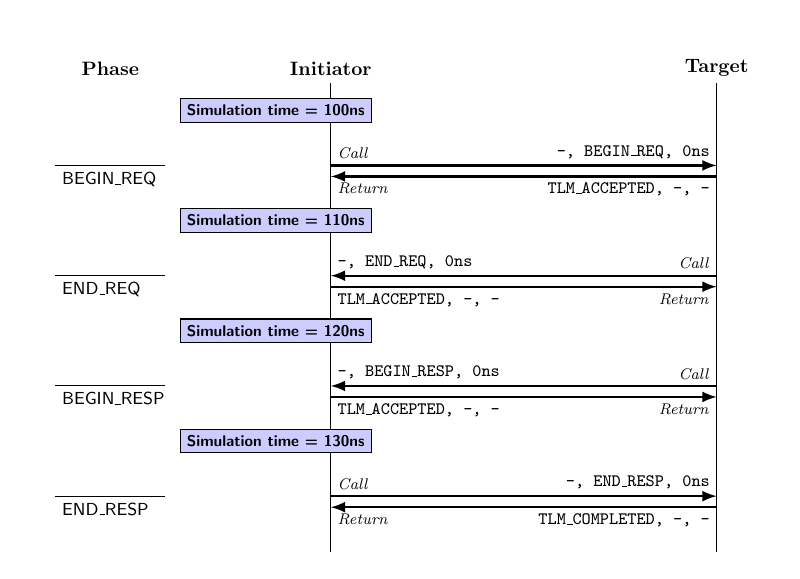
\begin{tikzpicture}[transform shape,scale=0.7]
		\clip (1.5,10.5) rectangle (15,20);
%		\draw[help lines] (0,0) grid (15,20);
		\path (3,19) coordinate (phase);
		\path (7,0) coordinate (llb);
		\path (7,19) coordinate (llt);
		\path (14,0) coordinate (rlb);
		\path (14,19) coordinate (rlt);
		
		\path (6,18.5) coordinate (100ns);
		\path (2,17.5) coordinate (breq_l);
		\path (4,17.5) coordinate (breq_r);
		\path (7,17.5) coordinate (breq_call_l);
		\path (14,17.5) coordinate (breq_call_r);
		\path (7,17.3) coordinate (breq_ret_l);
		\path (14,17.3) coordinate (breq_ret_r);

		\path (6,16.5) coordinate (110ns);
		\path (2,15.5) coordinate (ereq_l);
		\path (4,15.5) coordinate (ereq_r);
		\path (7,15.5) coordinate (ereq_call_l);
		\path (14,15.5) coordinate (ereq_call_r);
		\path (7, 15.3) coordinate (ereq_ret_l);
		\path (14,15.3) coordinate (ereq_ret_r);

		\path (6,14.5) coordinate (120ns);
		\path (2,13.5) coordinate (bresp_l);
		\path (4,13.5) coordinate (bresp_r);
		\path (7,13.5) coordinate (bresp_call_l);
		\path (14,13.5) coordinate (bresp_call_r);
		\path (7,13.3) coordinate (bresp_ret_l);
		\path (14,13.3) coordinate (bresp_ret_r);

		\path (6,12.5) coordinate (130ns);
		\path (2,11.5) coordinate (eresp_l);
		\path (4,11.5) coordinate (eresp_r);
		\path (7,11.5) coordinate (eresp_call_l);
		\path (14,11.5) coordinate (eresp_call_r);
		\path (7,11.3) coordinate (eresp_ret_l);
		\path (14,11.3) coordinate (eresp_ret_r);

		\draw (phase) node[above] {\textbf{Phase}};
		\draw (llb) -- (llt)
			node[above] {\textbf{Initiator}};
		\draw (rlb) -- (rlt)
			node[above] {\textbf{Target}};

		\draw (100ns) node [rectangle,draw,fill=blue!20] {\footnotesize \textsf{\textbf{Simulation time = 100ns}}};
		\draw (breq_l) node[below right] {\small \textsf{BEGIN\_REQ}} -- (breq_r);
		\draw[thick,-latex] (breq_call_l) -- (breq_call_r);
		\draw (breq_call_l) node[above right] {\footnotesize \emph{Call}};
		\draw (breq_call_r) node[above left] {\small \texttt{\textbf{-, BEGIN\_REQ, 0ns}}};
		\draw[thick,latex-] (breq_ret_l) -- (breq_ret_r);
		\draw (breq_ret_l) node[below right] {\footnotesize \emph{Return}};
		\draw (breq_ret_r) node[below left] {\small \texttt{\textbf{TLM\_ACCEPTED, -, -}}};

		\draw (110ns) node [rectangle,draw,fill=blue!20] {\footnotesize \textsf{\textbf{Simulation time = 110ns}}};
		\draw (ereq_l) node[below right] {\small \textsf{END\_REQ}} -- (ereq_r);
		\draw[thick,latex-] (ereq_call_l) -- (ereq_call_r);
		\draw (ereq_call_r) node[above left] {\footnotesize \emph{Call}};
		\draw (ereq_call_l) node[above right] {\small \texttt{\textbf{-, END\_REQ, 0ns}}};
		\draw[thick,-latex] (ereq_ret_l) -- (ereq_ret_r);
		\draw (ereq_ret_r) node[below left] {\footnotesize \emph{Return}};
		\draw (ereq_ret_l) node[below right] {\small \texttt{\textbf{TLM\_ACCEPTED, -, -}}};

		\draw (120ns) node [rectangle,draw,fill=blue!20] {\footnotesize \textsf{\textbf{Simulation time = 120ns}}};
		\draw (bresp_l) node[below right] {\small \textsf{BEGIN\_RESP}} -- (bresp_r);
		\draw[thick,latex-] (bresp_call_l) -- (bresp_call_r);
		\draw (bresp_call_r) node[above left] {\footnotesize \emph{Call}};
		\draw (bresp_call_l) node[above right] {\small \texttt{\textbf{-, BEGIN\_RESP, 0ns}}};
		\draw[thick,-latex] (bresp_ret_l) -- (bresp_ret_r);
		\draw (bresp_ret_r) node[below left] {\footnotesize \emph{Return}};
		\draw (bresp_ret_l) node[below right] {\small \texttt{\textbf{TLM\_ACCEPTED, -, -}}};

		\draw (130ns) node [rectangle,draw,fill=blue!20] {\footnotesize \textsf{\textbf{Simulation time = 130ns}}};
		\draw (eresp_l) node[below right] {\small \textsf{END\_RESP}} -- (eresp_r);
		\draw[thick,-latex] (eresp_call_l) -- (eresp_call_r);
		\draw (eresp_call_l) node[above right] {\footnotesize \emph{Call}};
		\draw (eresp_call_r) node[above left] {\small \texttt{\textbf{-, END\_RESP, 0ns}}};
		\draw[thick,latex-] (eresp_ret_l) -- (eresp_ret_r);
		\draw (eresp_ret_l) node[below right] {\footnotesize \emph{Return}};
		\draw (eresp_ret_r) node[below left] {\small \texttt{\textbf{TLM\_COMPLETED, -, -}}};

	\end{tikzpicture}
	\end{center}
\end{figure}


\end{frame}

}

\mode<article>{
Figure~\ref{fig:chart_at_using_backward_path} shows the message exchange that occur when using the approximately-timed coding style using the backward path.

\begin{figure}[h]
	\begin{center}
	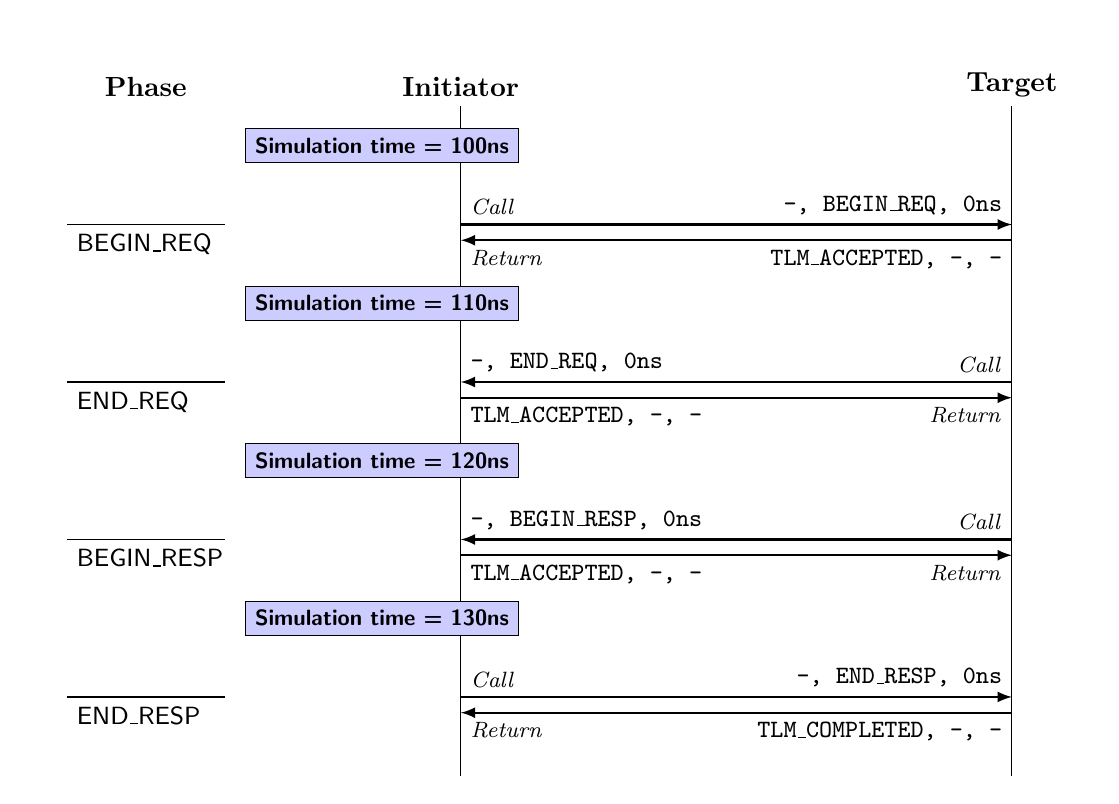
\begin{tikzpicture}
		\clip (1.5,10.5) rectangle (15,20);
%		\draw[help lines] (0,0) grid (15,20);
		\path (3,19) coordinate (phase);
		\path (7,0) coordinate (llb);
		\path (7,19) coordinate (llt);
		\path (14,0) coordinate (rlb);
		\path (14,19) coordinate (rlt);
		
		\path (6,18.5) coordinate (100ns);
		\path (2,17.5) coordinate (breq_l);
		\path (4,17.5) coordinate (breq_r);
		\path (7,17.5) coordinate (breq_call_l);
		\path (14,17.5) coordinate (breq_call_r);
		\path (7,17.3) coordinate (breq_ret_l);
		\path (14,17.3) coordinate (breq_ret_r);

		\path (6,16.5) coordinate (110ns);
		\path (2,15.5) coordinate (ereq_l);
		\path (4,15.5) coordinate (ereq_r);
		\path (7,15.5) coordinate (ereq_call_l);
		\path (14,15.5) coordinate (ereq_call_r);
		\path (7, 15.3) coordinate (ereq_ret_l);
		\path (14,15.3) coordinate (ereq_ret_r);

		\path (6,14.5) coordinate (120ns);
		\path (2,13.5) coordinate (bresp_l);
		\path (4,13.5) coordinate (bresp_r);
		\path (7,13.5) coordinate (bresp_call_l);
		\path (14,13.5) coordinate (bresp_call_r);
		\path (7,13.3) coordinate (bresp_ret_l);
		\path (14,13.3) coordinate (bresp_ret_r);

		\path (6,12.5) coordinate (130ns);
		\path (2,11.5) coordinate (eresp_l);
		\path (4,11.5) coordinate (eresp_r);
		\path (7,11.5) coordinate (eresp_call_l);
		\path (14,11.5) coordinate (eresp_call_r);
		\path (7,11.3) coordinate (eresp_ret_l);
		\path (14,11.3) coordinate (eresp_ret_r);

		\draw (phase) node[above] {\textbf{Phase}};
		\draw (llb) -- (llt)
			node[above] {\textbf{Initiator}};
		\draw (rlb) -- (rlt)
			node[above] {\textbf{Target}};

		\draw (100ns) node [rectangle,draw,fill=blue!20] {\footnotesize \textsf{\textbf{Simulation time = 100ns}}};
		\draw (breq_l) node[below right] {\small \textsf{BEGIN\_REQ}} -- (breq_r);
		\draw[thick,-latex] (breq_call_l) -- (breq_call_r);
		\draw (breq_call_l) node[above right] {\footnotesize \emph{Call}};
		\draw (breq_call_r) node[above left] {\small \texttt{\textbf{-, BEGIN\_REQ, 0ns}}};
		\draw[thick,latex-] (breq_ret_l) -- (breq_ret_r);
		\draw (breq_ret_l) node[below right] {\footnotesize \emph{Return}};
		\draw (breq_ret_r) node[below left] {\small \texttt{\textbf{TLM\_ACCEPTED, -, -}}};

		\draw (110ns) node [rectangle,draw,fill=blue!20] {\footnotesize \textsf{\textbf{Simulation time = 110ns}}};
		\draw (ereq_l) node[below right] {\small \textsf{END\_REQ}} -- (ereq_r);
		\draw[thick,latex-] (ereq_call_l) -- (ereq_call_r);
		\draw (ereq_call_r) node[above left] {\footnotesize \emph{Call}};
		\draw (ereq_call_l) node[above right] {\small \texttt{\textbf{-, END\_REQ, 0ns}}};
		\draw[thick,-latex] (ereq_ret_l) -- (ereq_ret_r);
		\draw (ereq_ret_r) node[below left] {\footnotesize \emph{Return}};
		\draw (ereq_ret_l) node[below right] {\small \texttt{\textbf{TLM\_ACCEPTED, -, -}}};

		\draw (120ns) node [rectangle,draw,fill=blue!20] {\footnotesize \textsf{\textbf{Simulation time = 120ns}}};
		\draw (bresp_l) node[below right] {\small \textsf{BEGIN\_RESP}} -- (bresp_r);
		\draw[thick,latex-] (bresp_call_l) -- (bresp_call_r);
		\draw (bresp_call_r) node[above left] {\footnotesize \emph{Call}};
		\draw (bresp_call_l) node[above right] {\small \texttt{\textbf{-, BEGIN\_RESP, 0ns}}};
		\draw[thick,-latex] (bresp_ret_l) -- (bresp_ret_r);
		\draw (bresp_ret_r) node[below left] {\footnotesize \emph{Return}};
		\draw (bresp_ret_l) node[below right] {\small \texttt{\textbf{TLM\_ACCEPTED, -, -}}};

		\draw (130ns) node [rectangle,draw,fill=blue!20] {\footnotesize \textsf{\textbf{Simulation time = 130ns}}};
		\draw (eresp_l) node[below right] {\small \textsf{END\_RESP}} -- (eresp_r);
		\draw[thick,-latex] (eresp_call_l) -- (eresp_call_r);
		\draw (eresp_call_l) node[above right] {\footnotesize \emph{Call}};
		\draw (eresp_call_r) node[above left] {\small \texttt{\textbf{-, END\_RESP, 0ns}}};
		\draw[thick,latex-] (eresp_ret_l) -- (eresp_ret_r);
		\draw (eresp_ret_l) node[below right] {\footnotesize \emph{Return}};
		\draw (eresp_ret_r) node[below left] {\small \texttt{\textbf{TLM\_COMPLETED, -, -}}};

	\end{tikzpicture}
	\end{center}
	\caption{Approximately-timed coding style using backward message chart.}
	\label{fig:chart_at_using_backward_path}
\end{figure}
}

\clearpage
\subsection{Approximately-timed with timing annotation}

\mode<presentation>{

\begin{frame}
	\frametitle{Approximately-timed with timing annotation}

\begin{figure}[h]
	\begin{center}
	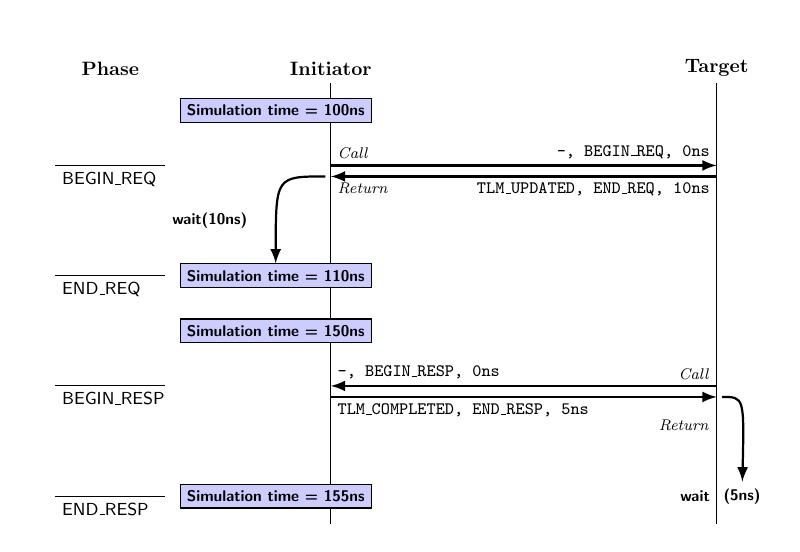
\begin{tikzpicture}[transform shape,scale=0.7]
		\clip (1.5,11) rectangle (15,20);
%		\draw[help lines] (0,0) grid (16,20);
		\path (3,19) coordinate (phase);
		\path (7,0) coordinate (llb);
		\path (7,19) coordinate (llt);
		\path (14,0) coordinate (rlb);
		\path (14,19) coordinate (rlt);
		
		\path (6,18.5) coordinate (100ns);
		\path (2,17.5) coordinate (breq_l);
		\path (4,17.5) coordinate (breq_r);
		\path (7,17.5) coordinate (breq_call_l);
		\path (14,17.5) coordinate (breq_call_r);
		\path (7,17.3) coordinate (breq_ret_l);
		\path (14,17.3) coordinate (breq_ret_r);
		
		\path (4,16.5) coordinate (wait10ns);

		\path (6,15.5) coordinate (110ns);
		\path (2,15.5) coordinate (ereq_l);
		\path (4,15.5) coordinate (ereq_r);

		\path (6,14.5) coordinate (150ns);
		\path (2,13.5) coordinate (bresp_l);
		\path (4,13.5) coordinate (bresp_r);
		\path (7,13.5) coordinate (bresp_call_l);
		\path (14,13.5) coordinate (bresp_call_r);
		\path (7,13.3) coordinate (bresp_ret_l);
		\path (14,13.3) coordinate (bresp_ret_r);

		\path (6,11.5) coordinate (155ns);
		\path (2,11.5) coordinate (eresp_l);
		\path (4,11.5) coordinate (eresp_r);
		\path (14,11.5) coordinate (wait5ns);

		\draw (phase) node[above] {\textbf{Phase}};
		\draw (llb) -- (llt)
			node[above] {\textbf{Initiator}};
		\draw (rlb) -- (rlt)
			node[above] {\textbf{Target}};

		\draw (100ns) node [rectangle,draw,fill=blue!20] {\footnotesize \textsf{\textbf{Simulation time = 100ns}}};
		\draw (breq_l) node[below right] {\small \textsf{BEGIN\_REQ}} -- (breq_r);
		\draw[thick,-latex] (breq_call_l) -- (breq_call_r);
		\draw (breq_call_l) node[above right] {\footnotesize \emph{Call}};
		\draw (breq_call_r) node[above left] {\small \texttt{\textbf{-, BEGIN\_REQ, 0ns}}};
		\draw[thick,latex-] (breq_ret_l) -- (breq_ret_r);
		\draw (breq_ret_l) node[below right] {\footnotesize \emph{Return}};
		\draw (breq_ret_r) node[below left] {\small \texttt{\textbf{TLM\_UPDATED, END\_REQ, 10ns}}};

		\draw (wait10ns) node(wait10ns_rect) [right] {\footnotesize \textsf{\textbf{wait(10ns)}}};
		
		\draw (110ns) node(sim110ns) [rectangle,draw,fill=blue!20] {\footnotesize \textsf{\textbf{Simulation time = 110ns}}};
		\path (breq_ret_l) +(-1,0) coordinate (control);
		\draw[thick,-latex] (breq_ret_l) +(-0.1,0) .. controls (control) .. (sim110ns)[above];

		\draw (ereq_l) node[below right] {\small \textsf{END\_REQ}} -- (ereq_r);

		\draw (150ns) node [rectangle,draw,fill=blue!20] {\footnotesize \textsf{\textbf{Simulation time = 150ns}}};
		\draw (bresp_l) node[below right] {\small \textsf{BEGIN\_RESP}} -- (bresp_r);
		\draw[thick,latex-] (bresp_call_l) -- (bresp_call_r);
		\draw (bresp_call_r) node[above left] {\footnotesize \emph{Call}};
		\draw (bresp_call_l) node[above right] {\small \texttt{\textbf{-, BEGIN\_RESP, 0ns}}};
		\draw[thick,-latex] (bresp_ret_l) -- (bresp_ret_r);
		\draw (bresp_ret_r) +(0,-0.3) node[below left] {\footnotesize \emph{Return}};
		\draw (bresp_ret_l) node[below right] {\small \texttt{\textbf{TLM\_COMPLETED, END\_RESP, 5ns}}};

		\draw (155ns) node [rectangle,draw,fill=blue!20] {\footnotesize \textsf{\textbf{Simulation time = 155ns}}};
		\draw (eresp_l) node[below right] {\small \textsf{END\_RESP}} -- (eresp_r);

		\draw (wait5ns) node [left] {\footnotesize \textsf{\textbf{wait}}};
		\draw (wait5ns) node(wait5ns_rect) [right] {\footnotesize \textsf{\textbf{(5ns)}}};
		\path (bresp_ret_r) +(0.5,0) coordinate (control);
		\draw[thick,-latex] (bresp_ret_r) +(0.1,0) .. controls (control) .. (wait5ns_rect)[above];
	\end{tikzpicture}
	\end{center}
\end{figure}

\end{frame}

}

\mode<article>{
Figure~\ref{fig:chart_at_with_timing_annotation} shows the message exchange that occur when using the approximately-timed coding style with timing annotations.

\begin{figure}[h]
	\begin{center}
	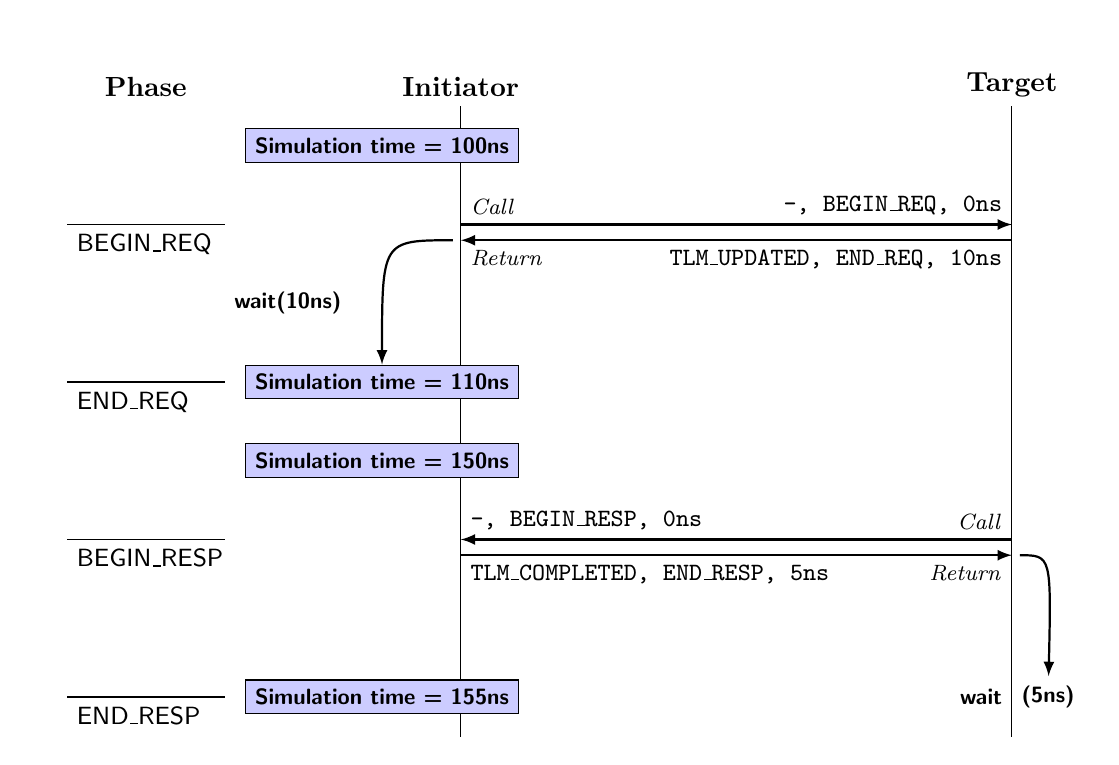
\begin{tikzpicture}
		\clip (1.5,11) rectangle (15,20);
%		\draw[help lines] (0,0) grid (16,20);
		\path (3,19) coordinate (phase);
		\path (7,0) coordinate (llb);
		\path (7,19) coordinate (llt);
		\path (14,0) coordinate (rlb);
		\path (14,19) coordinate (rlt);
		
		\path (6,18.5) coordinate (100ns);
		\path (2,17.5) coordinate (breq_l);
		\path (4,17.5) coordinate (breq_r);
		\path (7,17.5) coordinate (breq_call_l);
		\path (14,17.5) coordinate (breq_call_r);
		\path (7,17.3) coordinate (breq_ret_l);
		\path (14,17.3) coordinate (breq_ret_r);
		
		\path (4,16.5) coordinate (wait10ns);

		\path (6,15.5) coordinate (110ns);
		\path (2,15.5) coordinate (ereq_l);
		\path (4,15.5) coordinate (ereq_r);

		\path (6,14.5) coordinate (150ns);
		\path (2,13.5) coordinate (bresp_l);
		\path (4,13.5) coordinate (bresp_r);
		\path (7,13.5) coordinate (bresp_call_l);
		\path (14,13.5) coordinate (bresp_call_r);
		\path (7,13.3) coordinate (bresp_ret_l);
		\path (14,13.3) coordinate (bresp_ret_r);

		\path (6,11.5) coordinate (155ns);
		\path (2,11.5) coordinate (eresp_l);
		\path (4,11.5) coordinate (eresp_r);
		\path (14,11.5) coordinate (wait5ns);

		\draw (phase) node[above] {\textbf{Phase}};
		\draw (llb) -- (llt)
			node[above] {\textbf{Initiator}};
		\draw (rlb) -- (rlt)
			node[above] {\textbf{Target}};

		\draw (100ns) node [rectangle,draw,fill=blue!20] {\footnotesize \textsf{\textbf{Simulation time = 100ns}}};
		\draw (breq_l) node[below right] {\small \textsf{BEGIN\_REQ}} -- (breq_r);
		\draw[thick,-latex] (breq_call_l) -- (breq_call_r);
		\draw (breq_call_l) node[above right] {\footnotesize \emph{Call}};
		\draw (breq_call_r) node[above left] {\small \texttt{\textbf{-, BEGIN\_REQ, 0ns}}};
		\draw[thick,latex-] (breq_ret_l) -- (breq_ret_r);
		\draw (breq_ret_l) node[below right] {\footnotesize \emph{Return}};
		\draw (breq_ret_r) node[below left] {\small \texttt{\textbf{TLM\_UPDATED, END\_REQ, 10ns}}};

		\draw (wait10ns) node(wait10ns_rect) [right] {\footnotesize \textsf{\textbf{wait(10ns)}}};
		
		\draw (110ns) node(sim110ns) [rectangle,draw,fill=blue!20] {\footnotesize \textsf{\textbf{Simulation time = 110ns}}};
		\path (breq_ret_l) +(-1,0) coordinate (control);
		\draw[thick,-latex] (breq_ret_l) +(-0.1,0) .. controls (control) .. (sim110ns)[above];

		\draw (ereq_l) node[below right] {\small \textsf{END\_REQ}} -- (ereq_r);

		\draw (150ns) node [rectangle,draw,fill=blue!20] {\footnotesize \textsf{\textbf{Simulation time = 150ns}}};
		\draw (bresp_l) node[below right] {\small \textsf{BEGIN\_RESP}} -- (bresp_r);
		\draw[thick,latex-] (bresp_call_l) -- (bresp_call_r);
		\draw (bresp_call_r) node[above left] {\footnotesize \emph{Call}};
		\draw (bresp_call_l) node[above right] {\small \texttt{\textbf{-, BEGIN\_RESP, 0ns}}};
		\draw[thick,-latex] (bresp_ret_l) -- (bresp_ret_r);
		\draw (bresp_ret_r) node[below left] {\footnotesize \emph{Return}};
		\draw (bresp_ret_l) node[below right] {\small \texttt{\textbf{TLM\_COMPLETED, END\_RESP, 5ns}}};

		\draw (155ns) node [rectangle,draw,fill=blue!20] {\footnotesize \textsf{\textbf{Simulation time = 155ns}}};
		\draw (eresp_l) node[below right] {\small \textsf{END\_RESP}} -- (eresp_r);

		\draw (wait5ns) node [left] {\footnotesize \textsf{\textbf{wait}}};
		\draw (wait5ns) node(wait5ns_rect) [right] {\footnotesize \textsf{\textbf{(5ns)}}};
		\path (bresp_ret_r) +(0.5,0) coordinate (control);
		\draw[thick,-latex] (bresp_ret_r) +(0.1,0) .. controls (control) .. (wait5ns_rect)[above];
	\end{tikzpicture}
	\end{center}
	\caption{Approximately-timed coding style with timing annotation message chart.}
	\label{fig:chart_at_with_timing_annotation}
\end{figure}
}

% to do if we have time
% \subsection{Loosely- to approximately-timed adapter}

% to do if we have time
% \subsection{Approximately-timed initiator to loosely-timed target}


\mode<article>{
	\clearpage
}

\section{Other things}

\mode<presentation>{
\begin{frame}
	\frametitle{Other things}
	\begin{itemize}
		\item Things appearing in the current TLM 2.0 revision:
		\begin{itemize}
			\item Analysis interface and analysis ports.
			\item Adapters examples.
			\item Generic payload extension mechanism.
		\end{itemize}
		\item Things missing in the current TLM 2.0 revision:
		\begin{itemize}
			\item New standard protocols.
			\item Atomic transactions.
		\end{itemize}
	\end{itemize}
\end{frame}
}

\mode<article>{
In this tutorial we have learn the basics of TLM 2.0, but still some things remain if you really want to learn all about TLM 2.0. 
For example:
\begin{itemize}
	\item we have not talked about the analysis interface and analysis ports.
	They are intended to support the distribution of transactions to multiple 
components for analysis, meaning tasks such as checking for functional correctness or collecting functional coverage statistics.
	\item we have not seen examples on how to connect modules using different coding styles or TLM modules with cycle level modules. 
	Those are called adapters, and the TLM 2.0 provides some examples on how this can be done. 
	Usually it is done with a module that translates (the adapter) the coding style of the initiator module with the coding style of the second module.
	\item you have seen that the generic payload could be extended, however we have not talked about this because it could be considered as a non basic feature. 
	Again, the TLM 2.0 user manual explains how this can be done. 
\end{itemize}

There are even some things that the TLM 2.0 proposed standard does not explain. 
For example, new protocols (e.g., interrupts) can appear in future version of the standard.
Also the TLM 2.0 user manual explicitly states that the other capabilities like the atomic transactions might appear in future revisions of the Accellera TLM.

}


\input{tlm/exercise}


% \newpage

% \input{systemc_basics/basics_main}

% \newpage

% \input{tlm/tlm_main}

% \newpage

% \input{services/services_main}

\end{document}
